\documentclass[journal,10pt,onecolumn,compsocconf,]{IEEEtran}
%\documentclass[10pt,conference,compsocconf]{IEEEtran}

\usepackage[
backend=biber,
%style=alphabetic,
%sorting=ynt
]{biblatex}

\usepackage{float}
\usepackage{url}
\usepackage{graphicx}	% For figure environment
\usepackage{booktabs}
\usepackage{amsmath}

\usepackage{subcaption}
\usepackage{hyperref}
\usepackage{pdfpages}
\usepackage{enumerate}
\usepackage{subcaption}
\usepackage{cleveref}
\usepackage[newfloat]{minted}
\usepackage{stfloats}
\usepackage{cuted}

\captionsetup[listing]{position=top}

\clubpenalty=-100
%\windowpenalty=-100
\displaywidowpenalty=-100 
\linepenalty=5000
\clubpenalty=10000
\widowpenalty=10000
\displaywidowpenalty=10000

\renewcommand\thesection{Q\arabic{section}}

\addbibresource{ML4Healthcare.bib}
\defbibheading{references}{\section*{\large References}}

\setminted{%
breaklines,
frame=lines,
framesep=2mm,
fontsize=\footnotesize,
%mathescape,
linenos,
numbersep=5pt,
%frame=single,
numbersep=5pt,
xleftmargin=0pt,
}


\title{AI for Global Health using Natural Language Processing \\
\normalsize Project 2 for the Machine Learning for Health Care course (261-5120-00L) \\ \vspace*{20pt}
May 2023
}

\author{
  Sofie Daniëls, Aishwarya Melatur, Juraj Micko\\
  Group: 3 \\
  Department of Computer Science, ETH Zurich, Switzerland
}

\begin{document}
\pagenumbering{arabic}
\maketitle
\thispagestyle{plain}
\pagestyle{plain}



%\begin{abstract}
%  abc
%\end{abstract}

\section*{\large Part 1: Data exploration and pre-processing}
\section*{Q1: Preprocessing}
As a first step in our preprocessing pipeline, we enforced the data types of each column and dropped rows (or tweets) that did not follow such a table schema, or were duplicates. We found that about 126K tweets were duplicates, while about 53K tweets had invalid TweetIDs or invalid indices. Finally, we dropped about 113K tweets that contained the value 'NaN' in any of the columns, as a 'NaN' in a column can be indicative of data corruption for that tweet (as we had a very large dataset, we deemed it appropriate to have this stringent procedure). We thus end up with approximately 382K tweets out of an original 675K.

The dataset has quite a lot of challenges, even after dropping invalid rows as above: indeed, the TweetText column is very unstructured by nature, as it can contain URLs, emojis, user mentions, hashtags, misspellings, abbreviations, numbers, and variations in capitalisation. In order to counter this, we used a combination of regex and string functions to very efficiently strip the tweets of URLs, mentions, numbers, capitalisation, emojis, and to split hashtags into separate words, done in a few seconds. An example of this procedure is shown in Figure \ref{fig:prepr}, and the code snippet to achieve this is shown as well \cref{listing:p1-code1}.


\begin{listing*}[t]
\begin{minted}{python}
def rep(m):
   s=m.group(1)
   return ' '.join(re.split(r'(?=[A-Z])', s))


df_tweets['TweetText'] = [re.sub('((www\.[^\s]+)|(https?://[^\s]+))', '', x) for x in df_tweets['TweetText']] #remove url
df_tweets['TweetText'] = [re.sub('@[^\s]+', '' , x) for x in df_tweets['TweetText']] #remove mentions
df_tweets['TweetText'] = [x.encode("ascii", "ignore").decode() for x in df_tweets['TweetText']] # remove emojis
df_tweets['TweetText'] = [re.sub(r'#(\w+)', rep, x) for x in df_tweets['TweetText']] # split hashtags that are stuck together if they have case change: #iLovePotatoes becomes i love potatoes
df_tweets['TweetText'] = [re.sub(r'\W+', ' ', x) for x in df_tweets['TweetText']] # remove all characters that aren't alphanumerical - hashtag signs, punctuation, slashes...
df_tweets['TweetText'] = df_tweets["TweetText"].astype(str).str.replace('\d+', '') # remove numbers entirely
df_tweets['TweetText'] = df_tweets['TweetText'].str.lower() # remove all caps
\end{minted}
\caption{}
\label{listing:p1-code1}
\end{listing*}

\begin{figure}
    \centering
    \begin{subfigure}{0.5\columnwidth}
        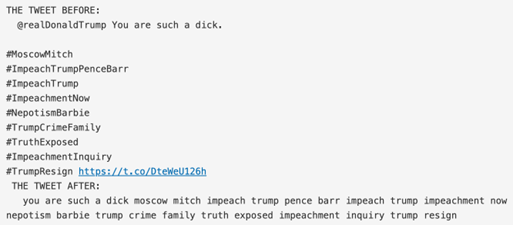
\includegraphics[width=1\textwidth]{images/prepr1.png}
    \end{subfigure}
    \caption{}
    \label{fig:prepr}
\end{figure}


We then tokenize each of the tweets by using Nltk's tokenize package, and then remove common English stopwords using Nltk's corpus package.
The column 'UserLocation' is used in Part 3, where we filtered tweets based on location, which we don't consider to be a part of preprocessing, however this is fully explained in Part 3. 

Finally, we choose to split our labels into two different columns, one for positive and for negative, as this is the obvious choice in order to use supervised models with two output heads, instead of being boxed into carrying out classification over 25 possible output labels (5*5).


\section*{Q2: Exploratory data analysis}
The most common unigrams and bigrams after preprocessing are shown in Figure \ref{fig:uni_bi_af}, and the ones before preprocessing are shown in Figure \ref{fig:uni_bi_bef} (after removing invalid rows as explained above). We show the two words in a bigram separated by an underscore, for better visualization in the word cloud. As expected, the observed unigrams and bigrams are worthless before preprocessing.

\begin{figure}
    \centering
    \begin{subfigure}{0.49\columnwidth}
        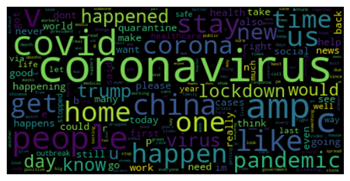
\includegraphics[width=1\textwidth]{images/uni_af.png}
    \end{subfigure}
    \centering
    \begin{subfigure}{0.49\columnwidth}
        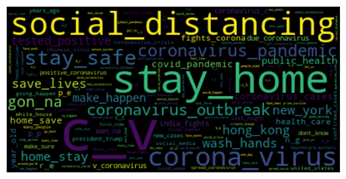
\includegraphics[width=1\textwidth]{images/bi_af.png}
    \end{subfigure}
    \caption{Most common unigrams (left) and most common bigrams (right) \textbf{after tweet preprocessing} shown as word clouds.}
    \label{fig:uni_bi_af}
\end{figure}

\begin{figure}
    \centering
    \begin{subfigure}{0.49\columnwidth}
        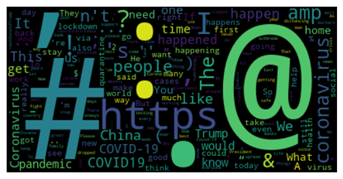
\includegraphics[width=1\textwidth]{images/uni_bef.png}
    \end{subfigure}
    \centering
    \begin{subfigure}{0.49\columnwidth}
        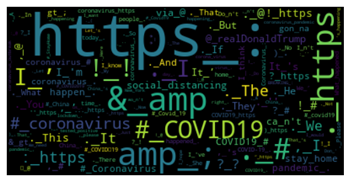
\includegraphics[width=1\textwidth]{images/bi_bef.png}
    \end{subfigure}
    \caption{Most common unigrams (left) and most common bigrams (right) \textbf{before tweet preprocessing} shown as word clouds.}
    \label{fig:uni_bi_bef}
\end{figure}

We then follow exactly the same procedure, but for extremely negative tweets, shown in Figure \ref{fig:uni_bi_neg}, and for extremely positive tweets, shown in Figure \ref{fig:uni_bi_pos}.

\begin{figure}
    \centering
    \begin{subfigure}{0.49\columnwidth}
        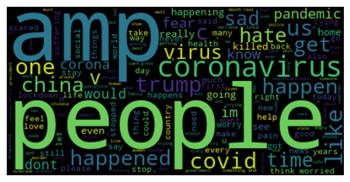
\includegraphics[width=1\textwidth]{images/uni_neg.png}
    \end{subfigure}
    \centering
    \begin{subfigure}{0.49\columnwidth}
        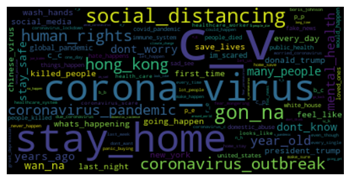
\includegraphics[width=1\textwidth]{images/bi_neg.png}
    \end{subfigure}
    \caption{Most common unigrams (left) and most common bigrams (right) for \textbf{extremely negative tweets} (negative\_sentiment $<$ -3).}
    \label{fig:uni_bi_neg}
\end{figure}

\begin{figure}
    \centering
    \begin{subfigure}{0.49\columnwidth}
        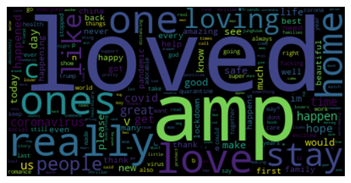
\includegraphics[width=1\textwidth]{images/uni_pos.png}
    \end{subfigure}
    \centering
    \begin{subfigure}{0.49\columnwidth}
        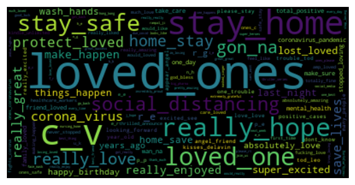
\includegraphics[width=1\textwidth]{images/bi_pos.png}
    \end{subfigure}
    \caption{Most common unigrams (left) and most common bigrams (right) for \textbf{extremely positive tweets} (positive\_sentiment $>$ 3).}
    \label{fig:uni_bi_pos}
\end{figure}

One can observe the unigram 'amp' in every unigram word cloud, however this is a keyword in social media websites (Accelerated Mobile Pages) and is thus not significant. We observe that the negative tweets have many terms with negative connotations on social media ('hate', 'sad', 'killed', 'Trump') but also neutral words like 'people', 'coronavirus', 'covid', which are words that do not appear in the extremely positive unigram word cloud. This shows that \textbf{tweets that mention the COVID-19 pandemic explicitly tend to be more overtly negative}. The extremely positive tweets' word clouds show very positive terms like 'loved', 'loving', 'stay home', 'stay safe', 'one', 'protect loved', and thus refer more to enforcing a positive attitude during the pandemic rather than the events of the pandemic themselves. 

We show the proportion of each sentiment label as a bubble chart along a grid defined by the labels (we take the absolute value of the negative sentiments, plotted here on the y-axis), in Figure \ref{fig:bubble}. We observe that \textbf{most of the labels are fairly neutral} (leaning towards the low end of the positive and negative values), however, the \textbf{more extreme tweets tend to be more negative than positive}: for example, (1, 4) is larger than (4, 1), where (x, y) refers to the bubble size of positive\_sentiment = x and negative\_sentiment = y. The dataset thus contains a very large proportion of mild tweets that are not particularly charged in sentiment.

\begin{figure}
    \centering
    \begin{subfigure}{0.7\columnwidth}
        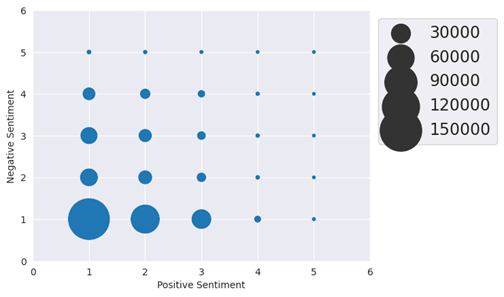
\includegraphics[width=1\textwidth]{images/bubble.png}
    \end{subfigure}
    \caption{Bubble chart of the number of positive and negative sentiments in the dataset.}
    \label{fig:bubble}
\end{figure}

\section*{Q3: Metric choice}
First, we introduce our interpretation of the problem. Predicting a value for either positive or negative sentiment is inherently a regression problem since the integer value is ordinal rather than categorical. In other words, the \textit{positive sentiment} value of $3$ semantically lies between the values of $2$ and $4$. The fact that these five categories of values (for both sentiments) are ordered brings the potential for models to perform better. However, in the problem description, we are given the task to solve a classification problem. Hence, we decided for the following approach:
\begin{enumerate}
    \item We are \textbf{solving a classification problem} as is asked for, in that our models return two integers in the suitable ranges (one for positive and negative sentiment), and during evaluation, we will treat each sentiment variable as categorical, therefore only allowing categorical metrics.
    \item Under the hood, we allow the models to capture the intrinsic regression problem, even though their output for evaluation will be one of five classes. This means that if it is suitable for a given model, we will naturally choose a regression loss function such as the mean squared error.
\end{enumerate}

\textbf{Metric choice.}
At first, we observe from \cref{fig:bubble} that classes are highly imbalanced, with classes closer to zero being orders of magnitude more likely (for both sentiment variables). Therefore an appropriate metric has to take the class imbalance into account. For a given class, a natural choice is first to evaluate the standard F1 score, calculated from Precision and Recall, and then calculate the Weighted F1 score which takes class imbalance into account. However, considering all 25 classes individually (= all combinations of permissible values for positive and negative sentiment variables) would not lead to a representative metric because a model that predicts both variables incorrectly would be rated the same as another model which predicts one of the variables correctly. Therefore, we decided to split the problem into two separate classification problems, one for each sentiment variable. We then calculate the Weighted F1 score for both variables and report their harmonic mean as the final metric. The harmonic mean, as opposed to the arithmetic mean, penalises models whose performance on the two variables is imbalanced.

\begin{listing*}[t]
\begin{minted}{python}
from sklearn.metrics import f1_score
from scipy.stats import hmean

def f1w_hm(pos_true, pos_pred, neg_true, neg_pred):
    """Harmonic mean of the weighted f1 scores for positive and negative sentiment variables.

    Args:
        pos_true (np.array): True labels of the positive sentiment variable.
        pos_pred (np.array): Predicted labels of the positive sentiment variable.
        neg_true (np.array): True labels of the negative sentiment variable.
        neg_pred (np.array): Predicted labels of the negative sentiment variable.
    """
    pos_f1 = f1_score(pos_true, pos_pred, average='weighted')
    neg_f1 = f1_score(neg_true, neg_pred, average='weighted')
    return hmean([pos_f1, neg_f1])
\end{minted}
\caption{The "Weighted-F1 HM" metric chosen for the two-output classification problem of predicting the positive and negative sentiment variables.}
\label{listing:p1-metric}
\end{listing*}

\Cref{listing:p1-metric} shows the primary metric that we call \textit{Weighted-F1 HM} that we will use to evaluate a model's performance on the given classification task, as well as to compare the predictive performance of different models.


\section*{Q4: Dataset splitting}

We choose to split our dataset in the following manner: we reserve 33\% of the dataset for the test set, and keep 67\% of the dataset for training and validation (where validation is typically 20\% of the training set, however this has been varied in our experiments). We also split by randomly shuffling the dataset, as we want the training to be agnostic to the timeframe. Indeed, in Figure \ref{fig:av_pos}, we plot the average of the positive labels in time (sorted timestamps, then averaged over 200 bins), and observe that this average isn't constant: there is a sharp fall towards the middle of the dataset. Thus, if we split our dataset without shuffling, we risk ending up with dataset splits that have different label proportions with respect to each other.

\begin{figure}
    \centering
    \begin{subfigure}{0.5\columnwidth}
        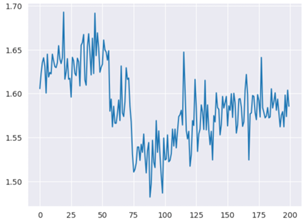
\includegraphics[width=1\textwidth]{images/av_pos.png}
    \end{subfigure}
    \caption{Average of positive labels over time, over 200 bins.}
    \label{fig:av_pos}
\end{figure}
\clearpage 
\section*{\large Part 2: NLP learning based methods}
\section*{VADER (5 pts)}

\subsection*{Q1: Briefly explain how VADER works (1 pt).}

According to VADER’s repository \cite{vader}, VADER (Valence Aware Dictionary and sEntiment Reasoner) is a rule-based sentiment analysis tool which uses a combination of lexicon-based and rule-based approaches to determine the sentiment polarity of a given text, and is especially designed for analyzing social media texts.

VADER uses a pre-built lexicon of words (validated by human raters) that have associated ‘valence’ scores: for each text, we find the words within that text that belong to the lexicon, sum their valence scores, adjust to VADER’s rules, and normalize to range between -1 and 1. This gives the compound score of the whole text, which we then threshold to get a ternary classification: positive, negative, or neutral.


\subsection*{Q2: Provide a code snippet detailing how to use it for this task (2 pts). In light of what you have learned about this method, reflect on pre-processing steps that might be unnecessary when using VADER.}

Code snippet \cref{listing:p2-code1} shows how we have used VADER for our use case. The lexicon that VADER uses is especially suitable for social media, and thus, there is no need to tokenize tweets and remove stopwords. However, it is still important to preprocess the tweet strings into clean text (by the methods shown in code snippet \cref{listing:p1-code1}).

\begin{listing*}
\begin{minted}{python}
from vaderSentiment.vaderSentiment import SentimentIntensityAnalyzer
sid_obj = SentimentIntensityAnalyzer()

def map_sentiment(compound_val):
   if compound_val >= 0.05:
       return 'positive'
   if compound_val <= - 0.05:
       return 'negative'
   else:
       return 'neutral'
df_tweets['vader_polarity'] = [sid_obj.polarity_scores(sentence) for sentence in df_tweets['TweetText']]
df_tweets['vader_decision'] = [map_sentiment(sentiment_dict['compound']) for sentiment_dict in df_tweets['vader_polarity']]

# convert our dataset to positive, negative and neutral labels by adding pos_sent and neg_sent
df_tweets['overall_sent_GT'] = df_tweets['pos_sent'].astype('int') + df_tweets['neg_sent'].astype('int')
def map_int(val):
   if val > 0:
       return 'positive'
   if val < 0:
       return 'negative'
   else:
       return 'neutral'
df_tweets['overall_sent_GT'] = [map_int(val) for val in df_tweets['overall_sent_GT']]

from sklearn.metrics import confusion_matrix
confusion_matrix(df_tweets['overall_sent_GT'], df_tweets['vader_decision'])
\end{minted}
\caption{Using VADER for our dataset, and converting our labels to three classes to measure the performance of VADER.}
\label{listing:p2-code1}
\end{listing*}


\subsection*{Q3: Apply this method to the TweetsCOV19 dataset and comment on the performance obtained (2 pts).}

We convert our ground truth labels into VADER-compatible labels by summing the positive and negative values, and taking the sign of the output. If the value is 0, it is neutral. While this approach is straightforward, it is quite naive (for example, a tweet that is labeled as (5, -5) classified as neutral in the same manner as a tweet labeled as (1, -1)). However, since extreme tweets (whose sentiment is higher than 3 for either positive or negative sentiments) are quite rare in the dataset, and there is no other straightforward heuristic for conversion, we choose this naive solution.

In Figure \ref{fig:vader}, we plot our confusion matrix between our VADER-converted ground truth labels, and the VADER predictions. 

\begin{figure}
    \centering
    \begin{subfigure}{0.49\columnwidth}
        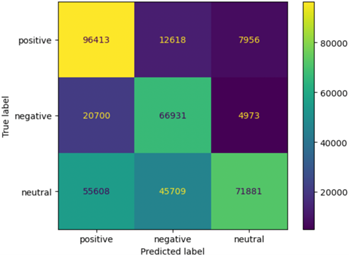
\includegraphics[width=1\textwidth]{images/vader_conf.png}
    \end{subfigure}
    \centering
    \begin{subfigure}{0.49\columnwidth}
        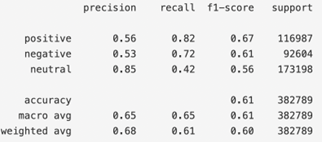
\includegraphics[width=1\textwidth]{images/vader_class.png}
    \end{subfigure}
    \caption{Confusion matrix and classification report of VADER’s predictions on the basis of our converted ground truth labels.}
    \label{fig:vader}
\end{figure}

While the performance evaluation of the VADER method might not seem impressive, it is important to remember that our ground truth labels are not adapted to the ternary classification task, and thus it is unwise to cast doubts on VADER’s predictions on this basis. Furthermore, the F1-score of every class is between 56\% and 67\%, and while these are not very high figures, they do show some agreement between our ground truth labels and the VADER method.

\clearpage 
\section*{Word Embeddings (20 pts)}


\subsection*{Q1: Bag of Words (BoW) (2 pts)}
\textit{Implement a Bag of Words embedding approach to create embeddings of the TweetsCOV19 dataset. Explain the methodology and provide a code snippet of the function used to produce these embeddings.}

Applying Bag of Words (BoW) \cite{bow} to tokens is the exact same as one-hot encoding of tokens.  We implemented our version of BoW using 'CountVectorizer' from scikit-klearn \cite{sklearn1, sklearn2}, as can be seen in Code Snippet \ref{listing:p2-bow}. To keep our implementation low in memory consumption, we choose to work with a vocabulary of size 250, which limits our token vectors to a size of 250.

\begin{listing*}
\begin{minted}{python}
from sklearn.feature_extraction.text import CountVectorizer
vectorizer = CountVectorizer(lowercase=False, max_features=250)
bow_matrix = vectorizer.fit_transform(df_tweets_preprocessed['unigram'].apply(" ".join))
\end{minted}
\caption{Short code snippet showing how to get the BoW vectors for each token.}
\label{listing:p2-bow}
\end{listing*}


\subsection*{Q2: TF-IDF (2 pts)}
\textit{Implement a TF-IDF \cite{tfidf} embedding approach to create embeddings of the TweetsCOV19 dataset. Explain the methodology and provide a code snippet of the function used to produce these embeddings.}

Similar to BoW, using term frequency–inverse document frequency (TF-IDF) \cite{tfidf} results in an embedding vector that has the same size as the vocabulary.  Instead of one-hot encoding, the entry of a word in a vector is directly related to its frequency in that tweet, and inversely related to the commonality of that word in general (i.e. the occurrence of that word in all tweets).  In Code Snippet \ref{listing:p2-tfidf}, we apply TfidfTransformer from scikit-learn \cite{sklearn1, sklearn2} to the BoW matrix we obtained in the previous question.

\begin{listing*}
\begin{minted}{python}
from sklearn.feature_extraction.text import TfidfTransformer
transformer = TfidfTransformer()
bow_matrix_tfidf = transformer.fit_transform(bow_matrix)
\end{minted}
\caption{Extension of the previous code snippet, applying tf-idf to the BoW vectors.}
\label{listing:p2-tfidf}
\end{listing*}

\subsection*{Q3: Word2Vec with CBOW or Skip-gram (2 pts)}
\textit{Implement a Word2Vec pre-trained embedding approach to create embeddings of the TweetsCOV19 dataset. Motivate your choice between CBOW or Skip-gram. Explain the methodology and provide a code snippet of the function used to produce these embeddings.}

Continuous Bag of Words (CBOW) \cite{cbowsgram} is a word embedding model that predicts a word by looking at the context (i.e. the surrounding words). Skip-gram \cite{cbowsgram}, on the other hand, does the opposite: it predicts the context of a word, by looking at the word itself. In general, Skip-gram is used more often, but CBOW is much faster, which makes sense, since you only predict a single word for the latter. Since we would like for our model to take context into account, we opt to use Skip-gram. Still, we will compare this with the performance of CBOW later on in question 8 and 9. For computational reasons (related to Q8), we limit the vector size of a token to 20 and therefore train the model from scratch instead of using a pre-trained model. In addition, we choose a context window of 3. We use the same vector and context window size for all subsequent models. The code for the respective functions can be found in Code Snippets \ref{listing:p2-cbow} and \ref{listing:p2-sgram}, and was written using functions from Gensim \cite{gensim}.

\begin{listing*}
\begin{minted}{python}
from gensim.models import Word2Vec
from gensim.models.callbacks import CallbackAny2Vec

# following class function from https://stackoverflow.com/questions/54888490/gensim-word2vec-print-log-loss
class callback(CallbackAny2Vec):
    def __init__(self):
        self.epoch = 0
        self.loss_to_be_subed = 0

    def on_epoch_end(self, model):
        loss = model.get_latest_training_loss()
        loss_now = loss - self.loss_to_be_subed
        self.loss_to_be_subed = loss
        print('Loss after epoch {}: {}'.format(self.epoch+1, loss_now))
        self.epoch += 1
        
context_size = 3 #hyperparameter
vec_size = 20 #300 most commonly used, according to https://arxiv.org/pdf/1812.04224.pdf

model_cbow = Word2Vec(min_count=1, vector_size=vec_size, window=context_size, sg=0, workers=20)
model_cbow.build_vocab(df_tweets_preprocessed['unigram'])
model_cbow.train(df_tweets_preprocessed['unigram'], epochs=15, total_examples=model_cbow.corpus_count,
                 compute_loss=True, callbacks=[callback()])
\end{minted}
\caption{Code snippet showing how the CBOW model was constructed and trained. The loss function was printed after every epoch.}
\label{listing:p2-cbow}
\end{listing*}

\begin{listing*}
\begin{minted}{python}
model_sgram = Word2Vec(min_count=1, vector_size=vec_size, window=context_size, sg=1, workers=20)
model_sgram.build_vocab(df_tweets_preprocessed['unigram'])
model_sgram.train(df_tweets_preprocessed['unigram'], epochs=15, total_examples=model_sgram.corpus_count,
                  compute_loss=True, callbacks=[callback()])
\end{minted}
\caption{Code snippet showing how the Skip-gram model was constructed and trained. Using the function from the previous code snippet, the loss function was printed after every epoch.}
\label{listing:p2-sgram}
\end{listing*}


\subsection*{Q4: GloVe (2 pts)}
\textit{Implement a GloVe pre-trained embedding approach to create embeddings of the TweetsCOV19 dataset. Explain the methodology and provide a code snippet of the function used to produce these embeddings.}
\begin{listing*}
\begin{minted}{python}
! pip install glove-python-binary

from glove import Glove, Corpus
from gensim.models.keyedvectors import KeyedVectors
from gensim.scripts.glove2word2vec import glove2word2vec

corpus = Corpus() 
corpus.fit(df_tweets_preprocessed['unigram'], window=context_size)
model_glove = Glove(no_components=vec_size, learning_rate=0.05, alpha=0.75, max_count=100, max_loss=10.0)
model_glove.fit(corpus.matrix, epochs=15, no_threads=16, verbose=True)
model_glove.add_dictionary(corpus.dictionary)

#from https://stackoverflow.com/questions/55693318/encoding-problem-while-training-my-own-glove-model
with open("word_embedding/results_glove.txt", "w") as f:
    for word in model_glove.dictionary:
        f.write(word)
        f.write(" ")
        for i in range(0, vec_size):
            f.write(str(model_glove.word_vectors[model_glove.dictionary[word]][i]))
            f.write(" ")
        f.write("\n")


glove2word2vec(glove_input_file="word_embedding/results_glove.txt", word2vec_output_file="word_embedding/gensim_glove_vectors.txt")    

model_glove_gensim = KeyedVectors.load_word2vec_format("word_embedding/gensim_glove_vectors.txt", binary=False)
\end{minted}
\caption{Code snippet showing how the GloVe embedding model was trained. We used the glove-python-binary library \cite{glovegit} in combination with Gensim \cite{gensim}.}
\label{listing:p2-glove}
\end{listing*}

GloVe \cite{glove} is an embedding method that counts how often a word occurs in a certain context. It combines these findings into a so-called co-occurrence matrix, which is then approximated by a lower-dimensional matrix to limit the vector size of the embeddings.
We use the library 'glove-python-binary' for our code \cite{glovegit}, as can be seen in Code Snippet \ref{listing:p2-glove}.

\subsection*{Q5: FastText (2 pts)}
\textit{Implement a FastText pre-trained embedding approach to create embedding of the TweetsCOV19 dataset. Explain the methodology and provide a code
snippet of the function used to produce these embeddings.}


\begin{listing*}
\begin{minted}{python}
from gensim.models import FastText

sg = 1 #cbow=0, skipgram=1
model_ft = FastText(min_count=1, vector_size=vec_size, window=context_size, workers=20, sg=0)
model_ft.build_vocab(df_tweets_preprocessed['unigram'])
model_ft.train(df_tweets_preprocessed['unigram'], epochs=15, total_examples=model_ft.corpus_count)
model_ft.save("word_embedding/fasttext.model")
\end{minted}
\caption{Code used for training the FastText model. Like with CBOW and Skip-gram, the Gensim library was used \cite{gensim}.}
\label{listing:p2-fasttext}
\end{listing*}

Different from the previous embedding methods, FastText \cite{fasttext} uses n-grams as input for training to ensure that uncommon and unseen words can still be embedded. Previous methods try to find a unique embedding for each word, but since FastText cares about the morphological similarity of words through n-grams, it can handle out-of-vocabulary (OOV) words. Training follows a similar fashion to the word2vec models mentioned earlier \cite{cbowsgram}.
The code can be found in Code Snippet \ref{listing:p2-fasttext}

\subsection*{Q6: Visualization of embeddings (2 pts)}
\textit{Perform a qualitative comparison of the quality of the semantic content of each embedding approach. For example, visualize the location using dimensionality reduction techniques (e.g., PCA, t-SNE, UMAP), of negative/positive samples, or tweets containing specific words, in the latent space. Compare your visualization of each method and explain whether you can anticipate any differences in downstream performance as a result. \cite{tsne, umap}}

We visualize our word embeddings both by the positive/negative score of tokens, but also by the keywords used for filtering the tweets.

For the first method, we us a list of over 1400 positive and negative words from \cite{AFINN}, each with a rank, and map their embeddings into the latent space. We hope to see that all of the previously implemented embedding methods allow us to easily discern words with a positive meaning from words with a negative meaning.

For the second method, we use the keywords used for filtering the TweetCov19 dataset \cite{tweetsdataset}, and again map the embeddings into the latent space. This time, we hope to see similar words clustered or located close to one another, and words with completely different meanings further away from each other.

Note that we only use keywords and positive/negative words that are in the vocabulary of the trained embedding model. This means that for both our BoW and TF-IDF model, most words are filtered out (since the entire vocabulary only has size 250), as you can see in Figure \ref{fig:bow_viz} and \ref{fig:tfidf_viz}. This will impede our downstream classifiers in finding the correct sentiment scores, but instead greatly speeds up training, since the feature size is significantly reduced.

\begin{figure}
 \centering
 \begin{subfigure}{\columnwidth}
 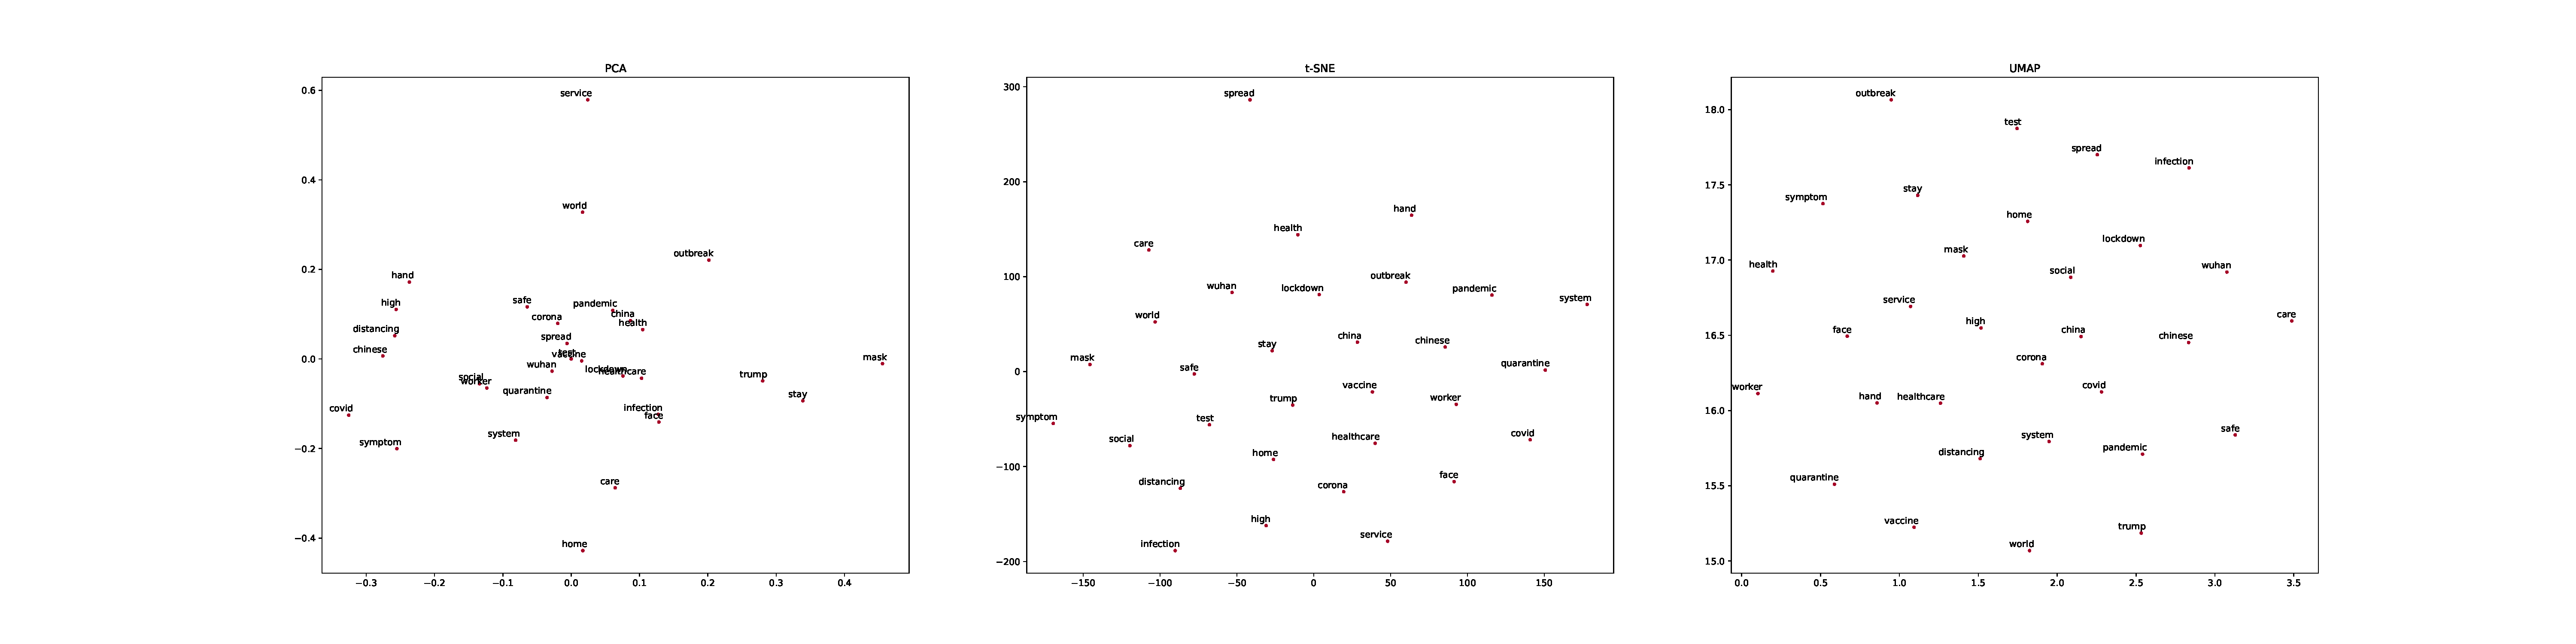
\includegraphics[width=1\textwidth]{images/keywords_bow.pdf}
  \caption{Distribution of keywords used to select tweets for the TweetsCOV19 dataset.}
 \label{fig:bow_key}
 \end{subfigure}
 \centering
 \begin{subfigure}{\columnwidth}
 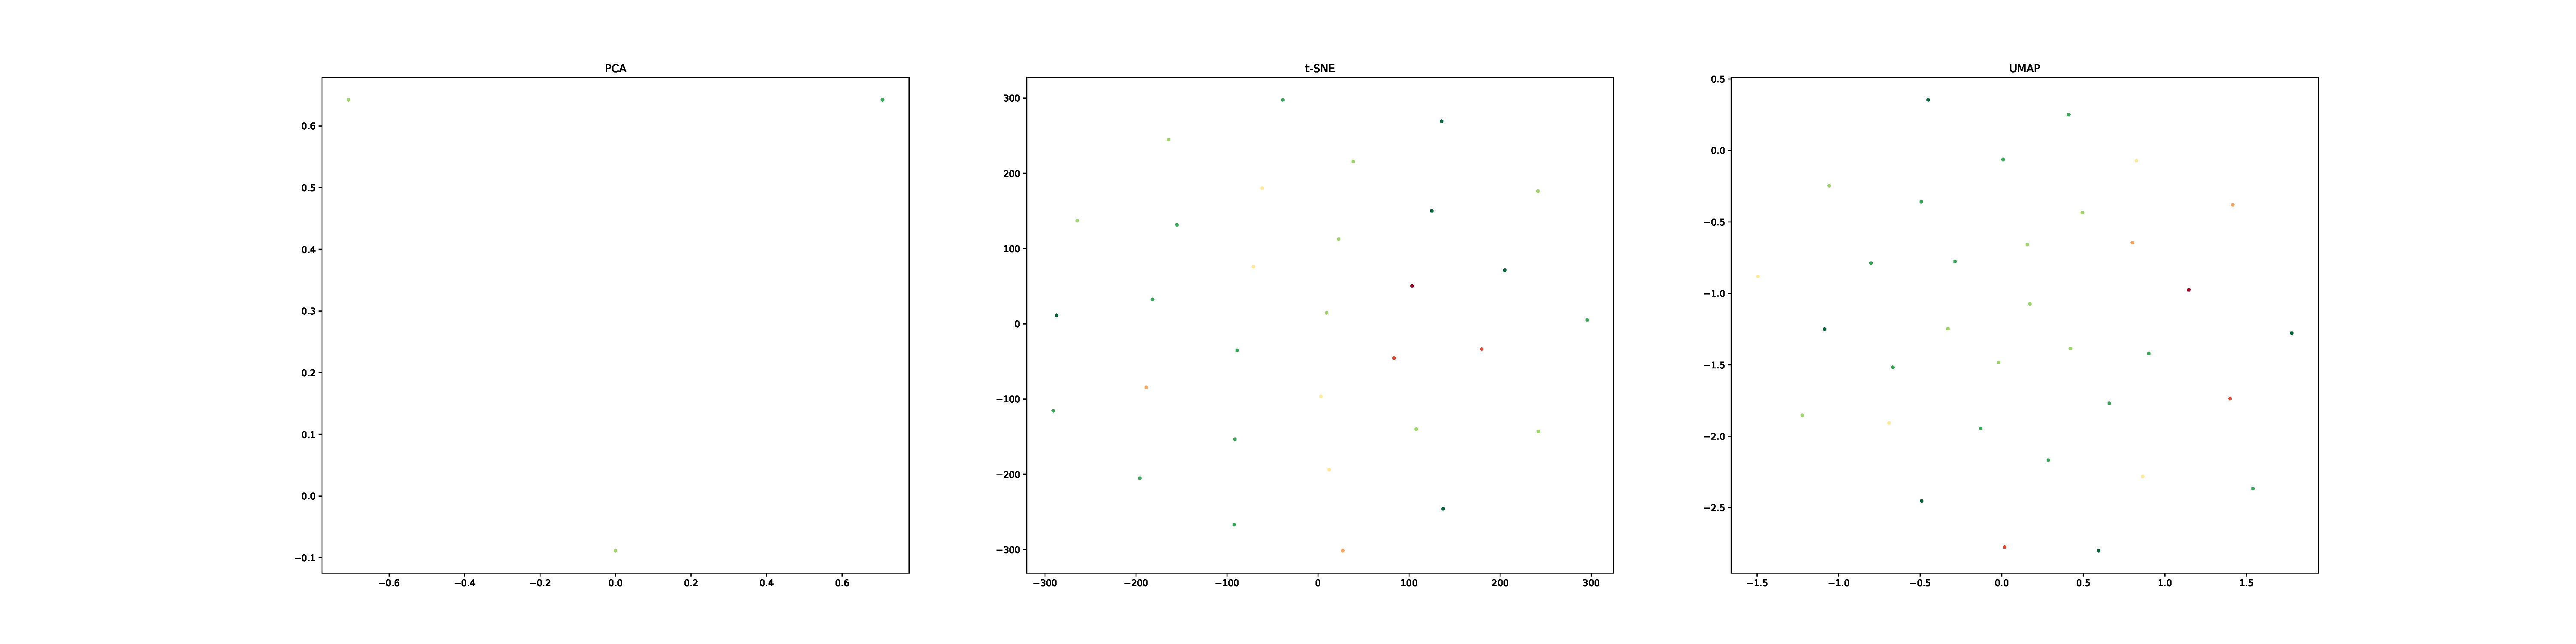
\includegraphics[width=1\textwidth]{images/keywords_bow_posneg.pdf}
  \caption{Distribution of positive and negative words from the AFINN-96 dataset.}
  \label{fig:bow_posneg}
 \end{subfigure}
 \caption{Visualization of BoW embedding of keywords and positive/negative words with PCA, t-SNE, and UMAP.}
 \label{fig:bow_viz}
\end{figure}

\begin{figure}
 \centering
 \begin{subfigure}{\columnwidth}
 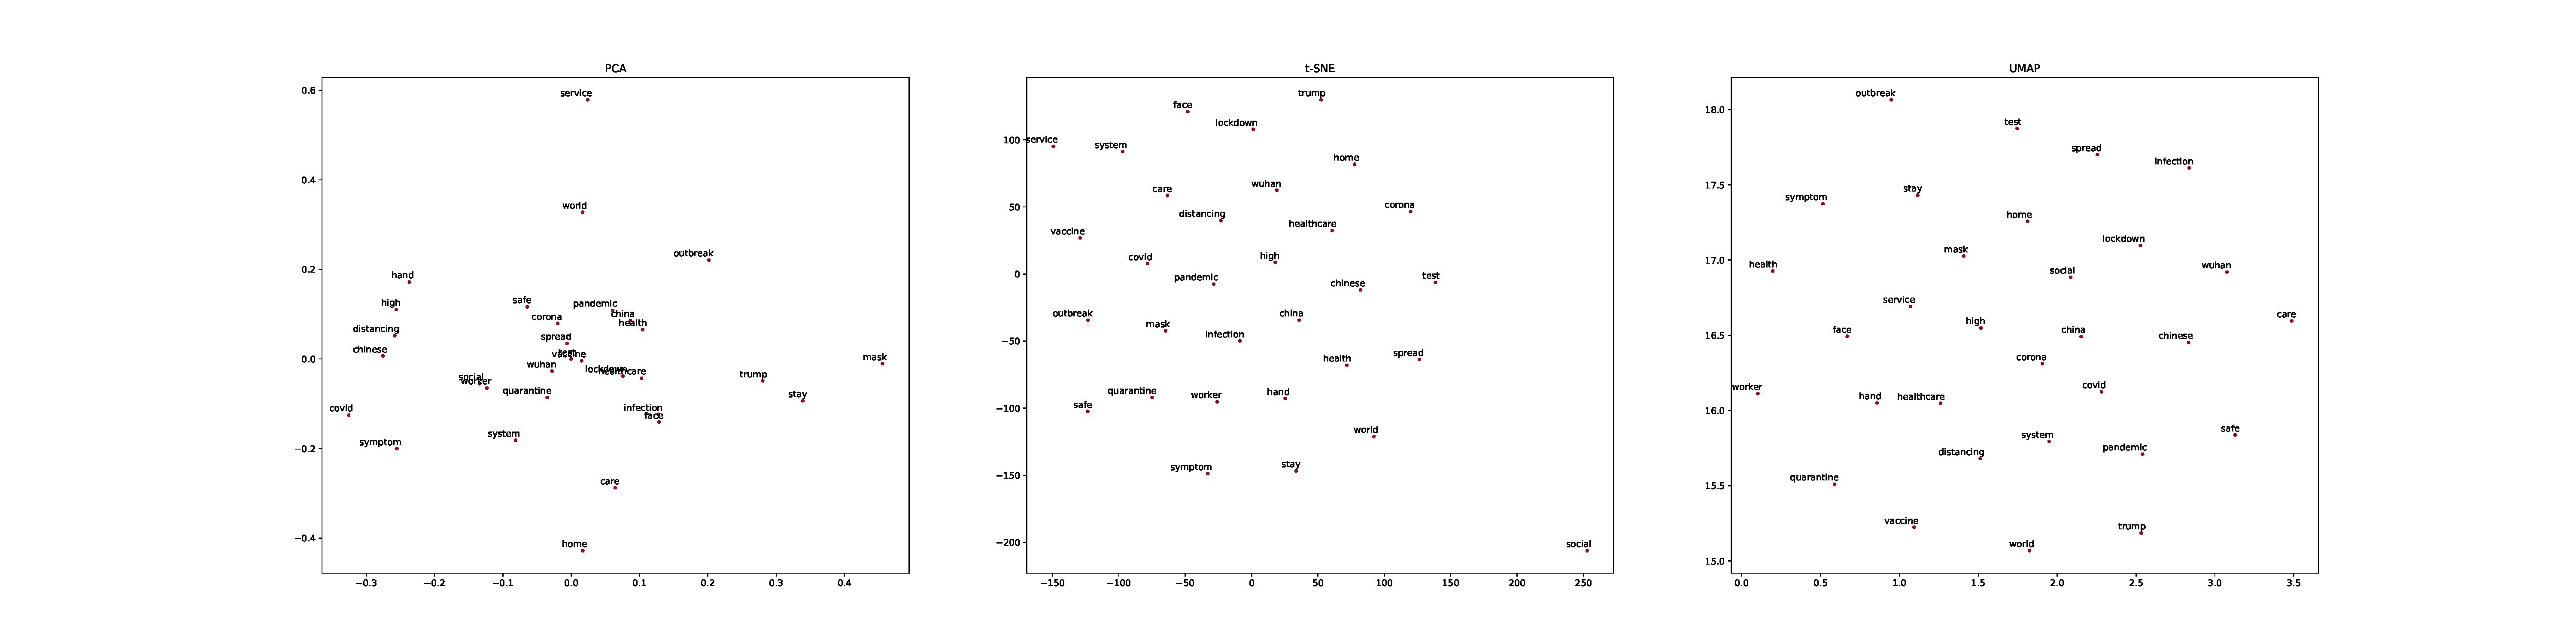
\includegraphics[width=1\textwidth]{images/keywords_tfidf.pdf}
 \caption{Distribution of keywords used to select tweets for the TweetsCOV19 dataset.}
 \label{fig:tfidf_key}
 \end{subfigure}
 \centering
 \begin{subfigure}{\columnwidth}
 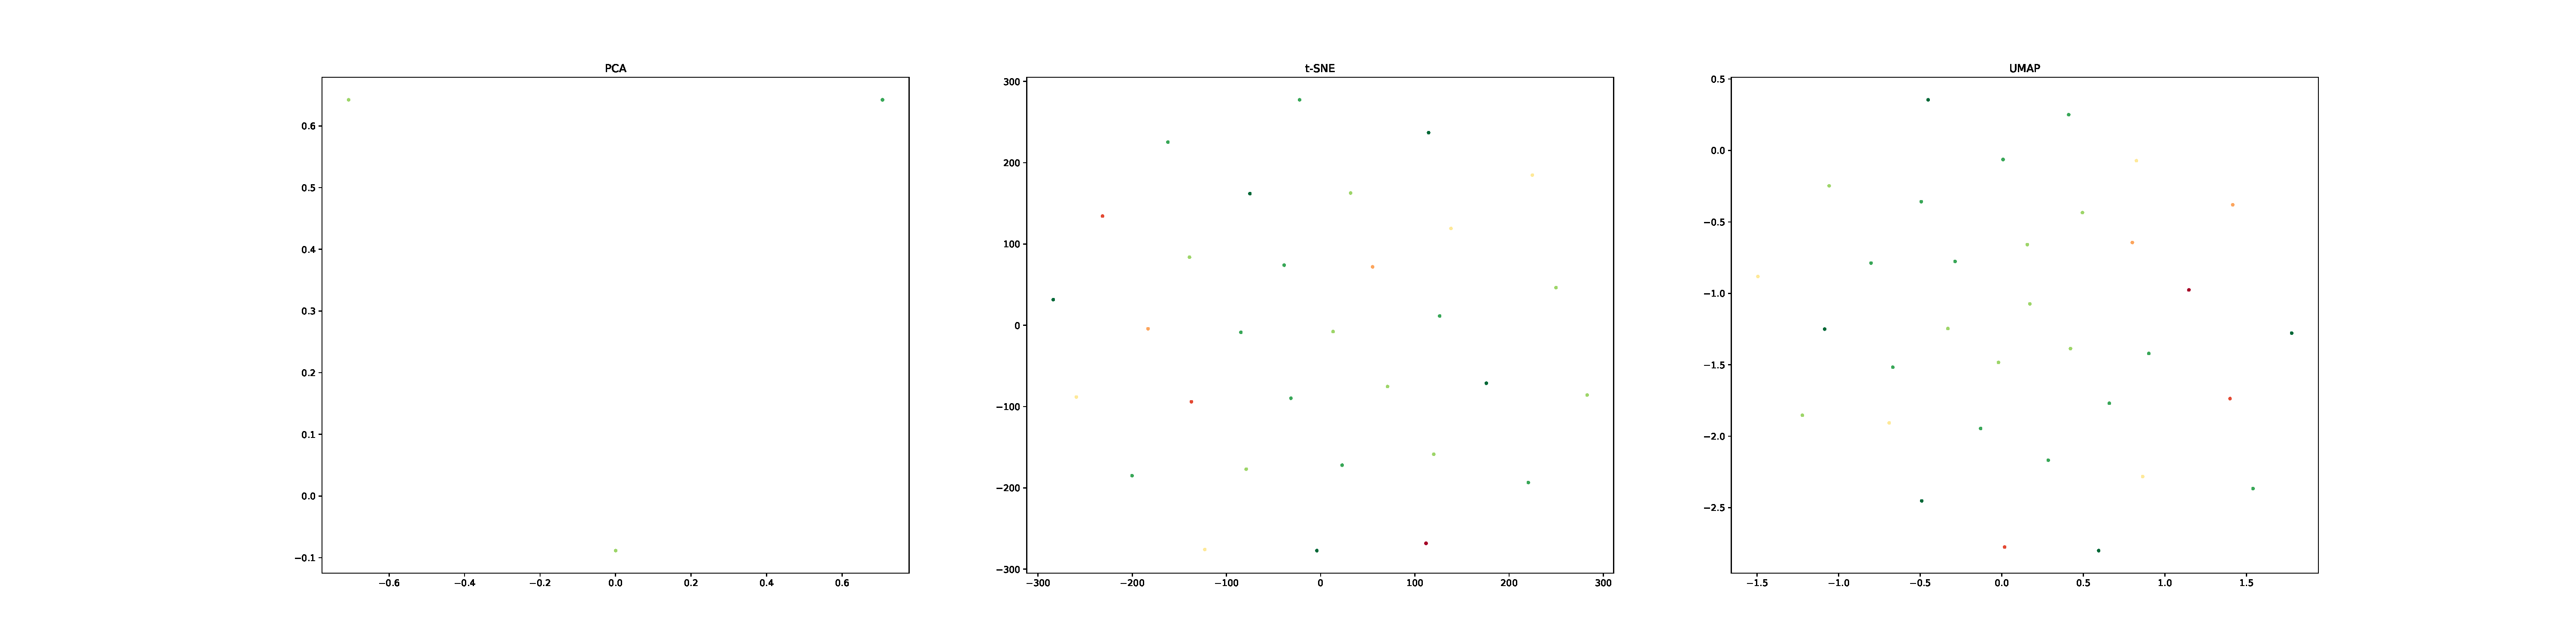
\includegraphics[width=1\textwidth]{images/keywords_tfidf_posneg.pdf}
 \caption{Distribution of positive and negative words from the AFINN-96 dataset.}
  \label{fig:tfidf_posneg}
 \end{subfigure}
 \caption{Visualization of TF-IDF embedding of keywords and positive/negative words with PCA, t-SNE, and UMAP.}
 \label{fig:tfidf_viz}
\end{figure}

\begin{figure}
 \centering
 \begin{subfigure}{\columnwidth}
 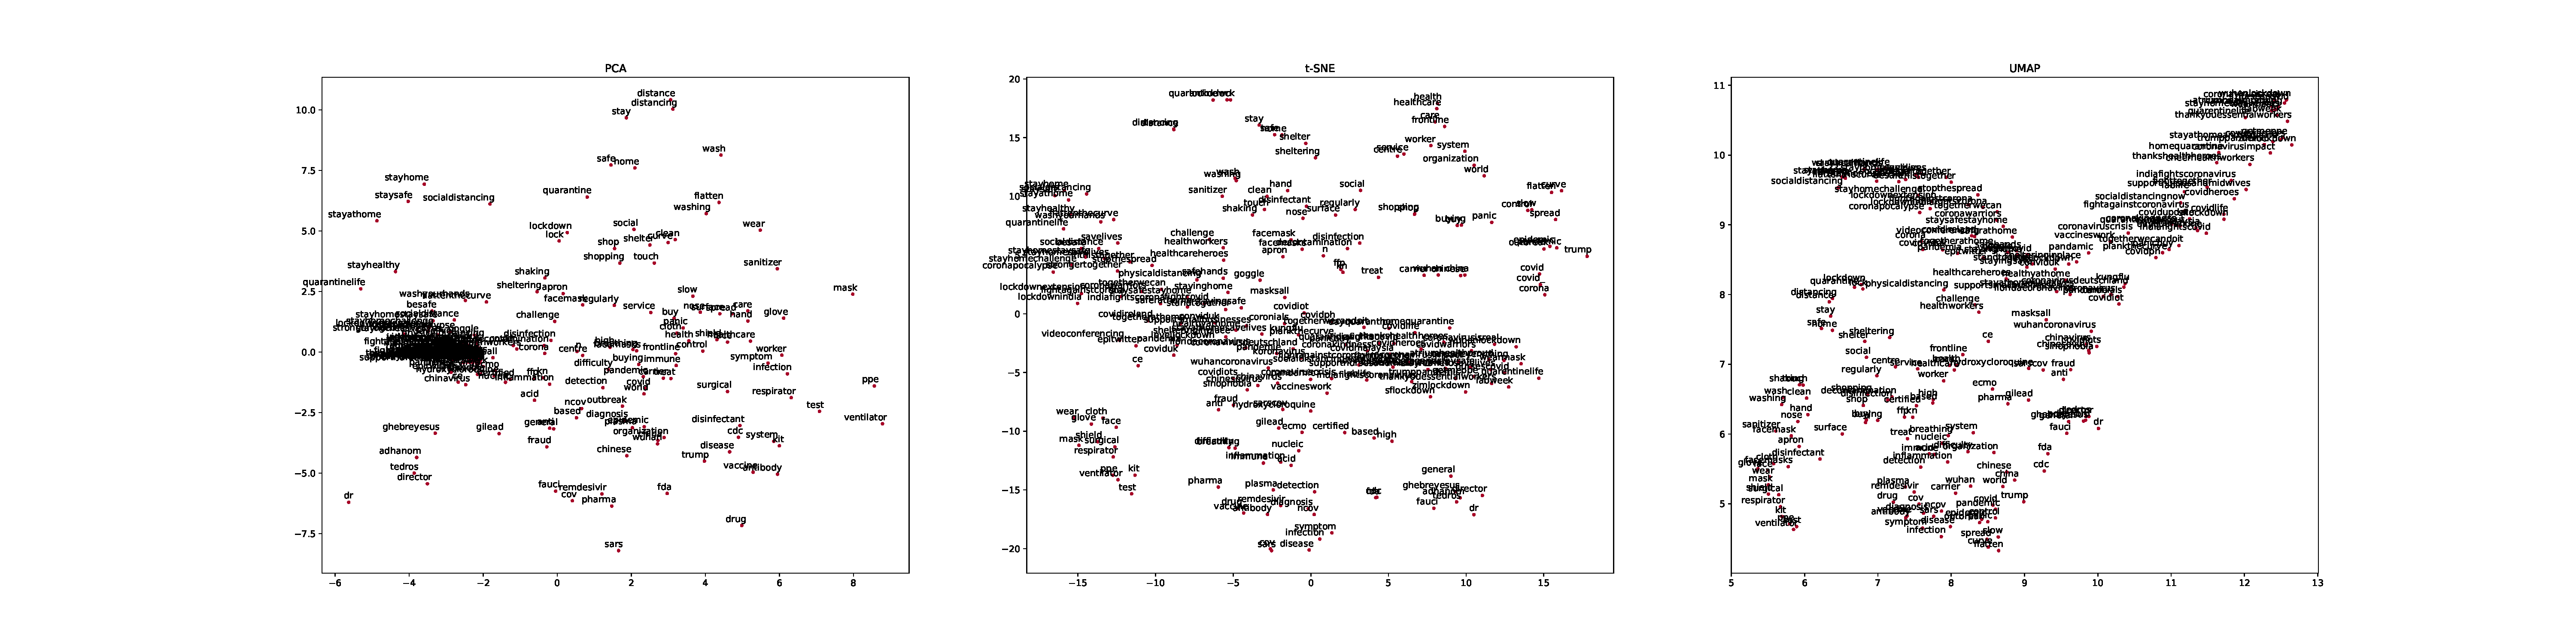
\includegraphics[width=1\textwidth]{images/keywords_cbow.pdf}
 \caption{Distribution of keywords used to select tweets for the TweetsCOV19 dataset.}
 \label{fig:cbow_key}
 \end{subfigure}
 \centering
 \begin{subfigure}{\columnwidth}
 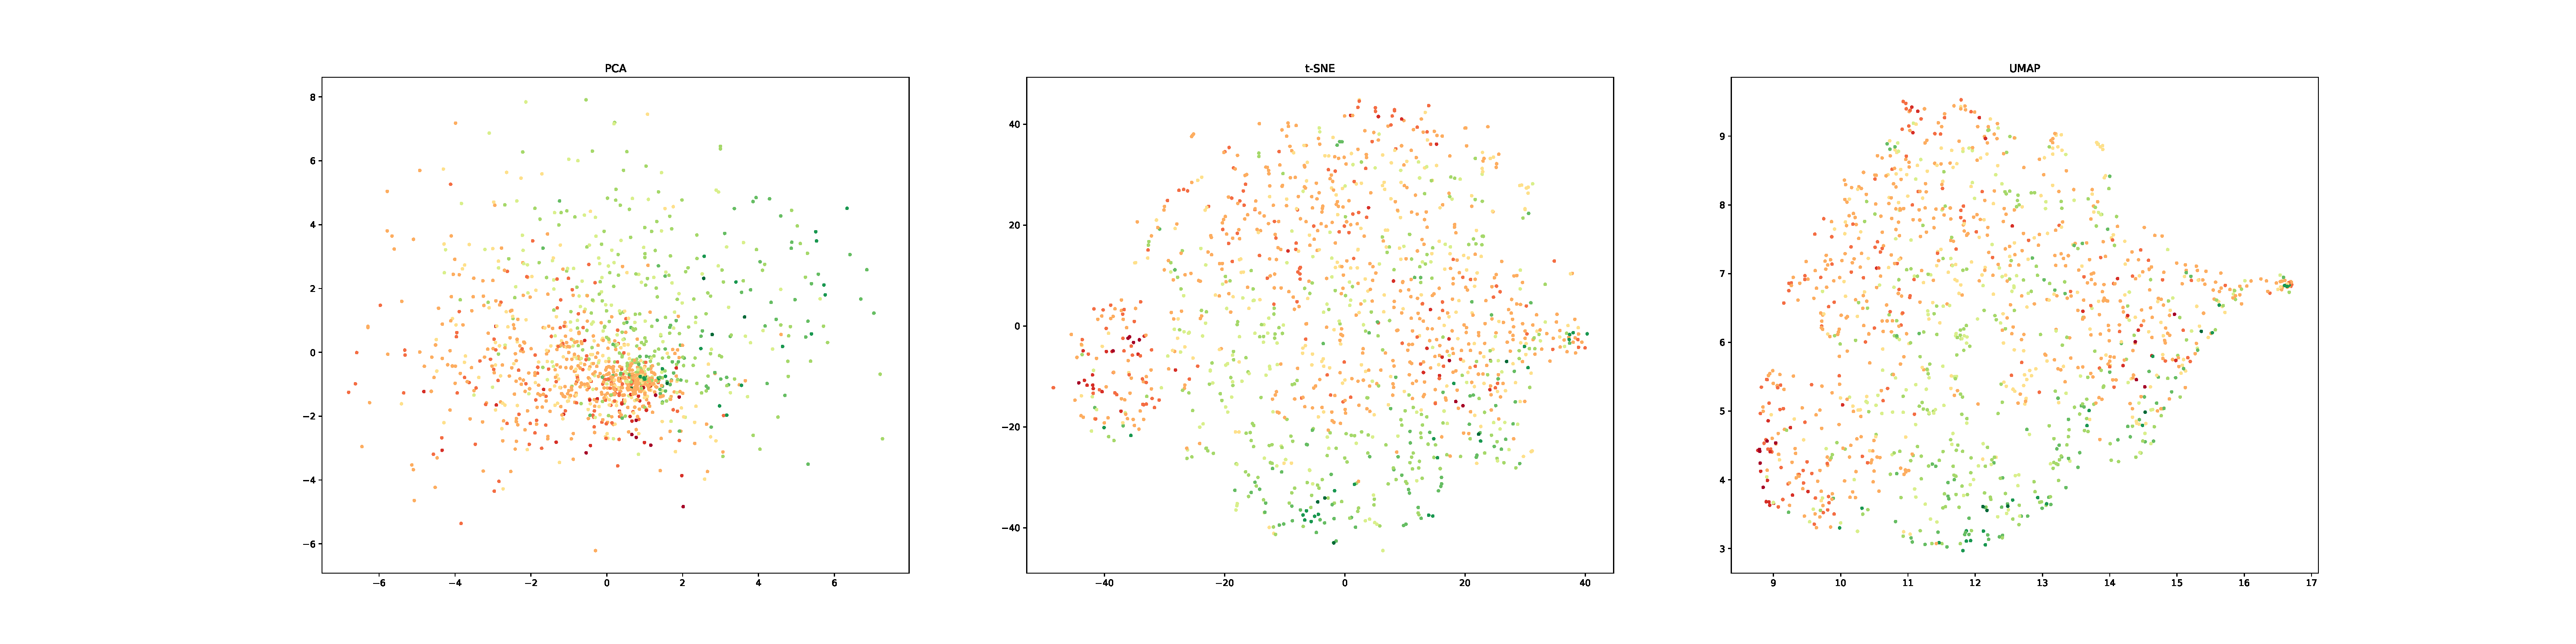
\includegraphics[width=1\textwidth]{images/keywords_cbow_posneg.pdf}
 \caption{Distribution of positive and negative words from the AFINN-96 dataset.}
  \label{fig:cbow_posneg}
 \end{subfigure}
 \caption{Visualization of CBOW embedding of keywords and positive/negative words with PCA, t-SNE, and UMAP.}
 \label{fig:cbow_viz}
\end{figure}

\begin{figure}
 \centering
 \begin{subfigure}{\columnwidth}
 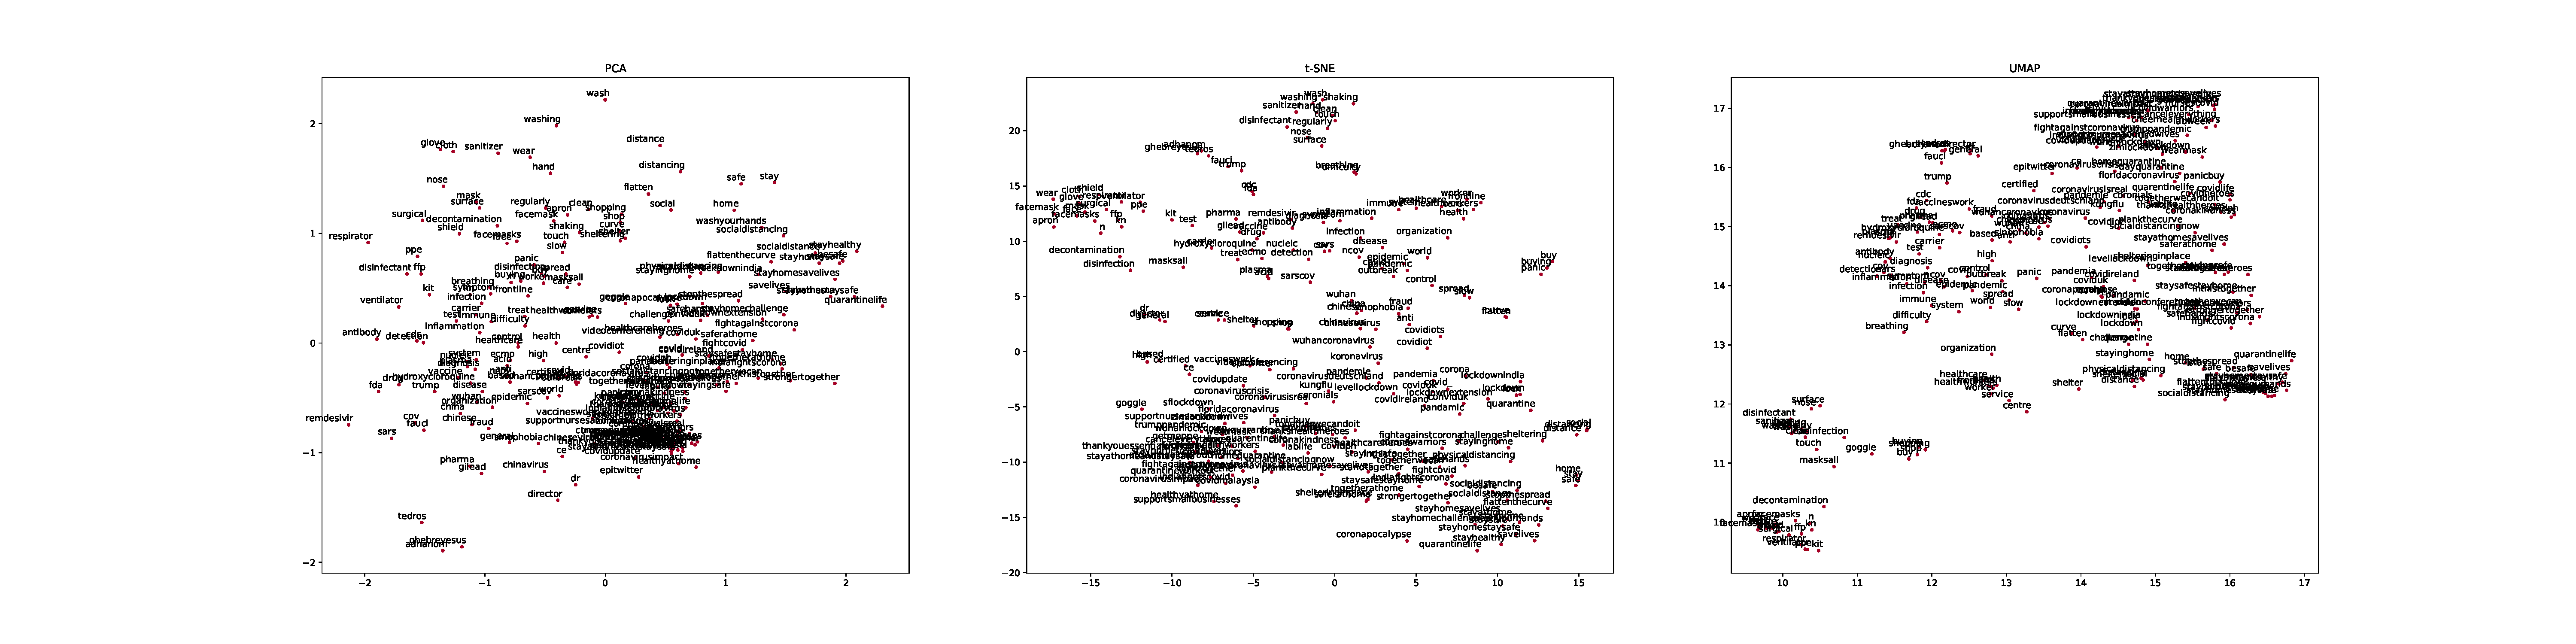
\includegraphics[width=1\textwidth]{images/keywords_sgram.pdf}
 \caption{Distribution of keywords used to select tweets for the TweetsCOV19 dataset.}
 \label{fig:sgram_key}
 \end{subfigure}
 \centering
 \begin{subfigure}{\columnwidth}
 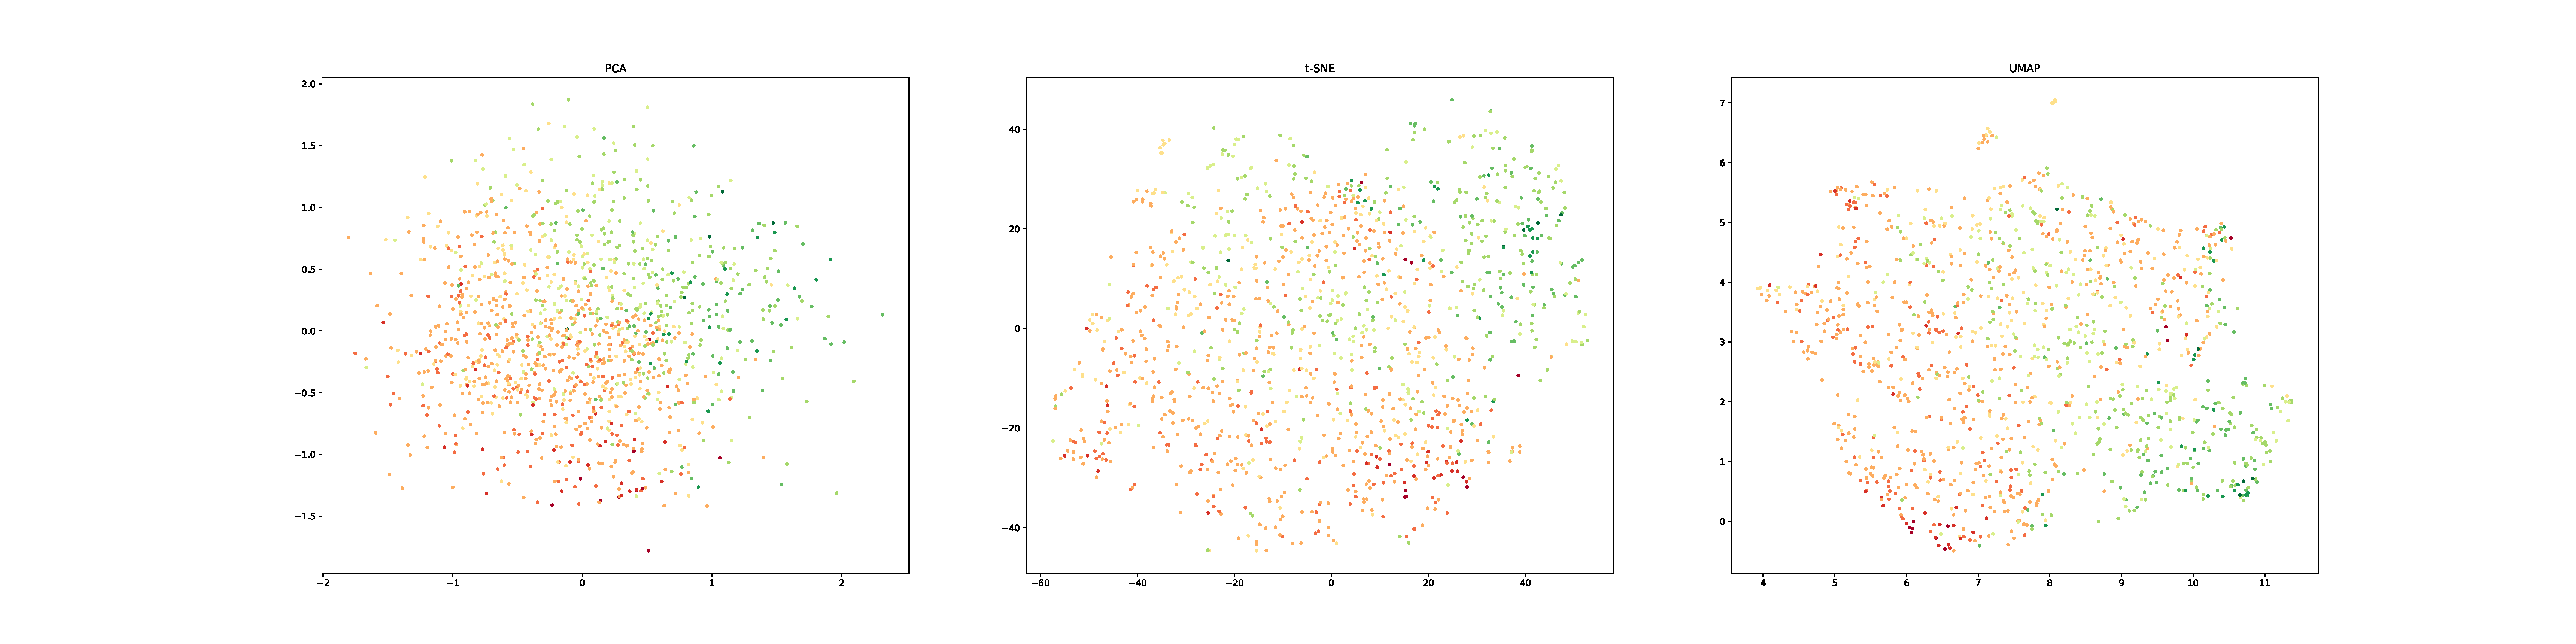
\includegraphics[width=1\textwidth]{images/keywords_sgram_posneg.pdf}
 \caption{Distribution of positive and negative words from the AFINN-96 dataset.}
  \label{fig:sgram_posneg}
 \end{subfigure}
 \caption{Visualization of Skip-gram embedding of keywords and positive/negative words with PCA, t-SNE, and UMAP.}
 \label{fig:sgram_viz}
\end{figure}

\begin{figure}
 \centering
 \begin{subfigure}{\columnwidth}
 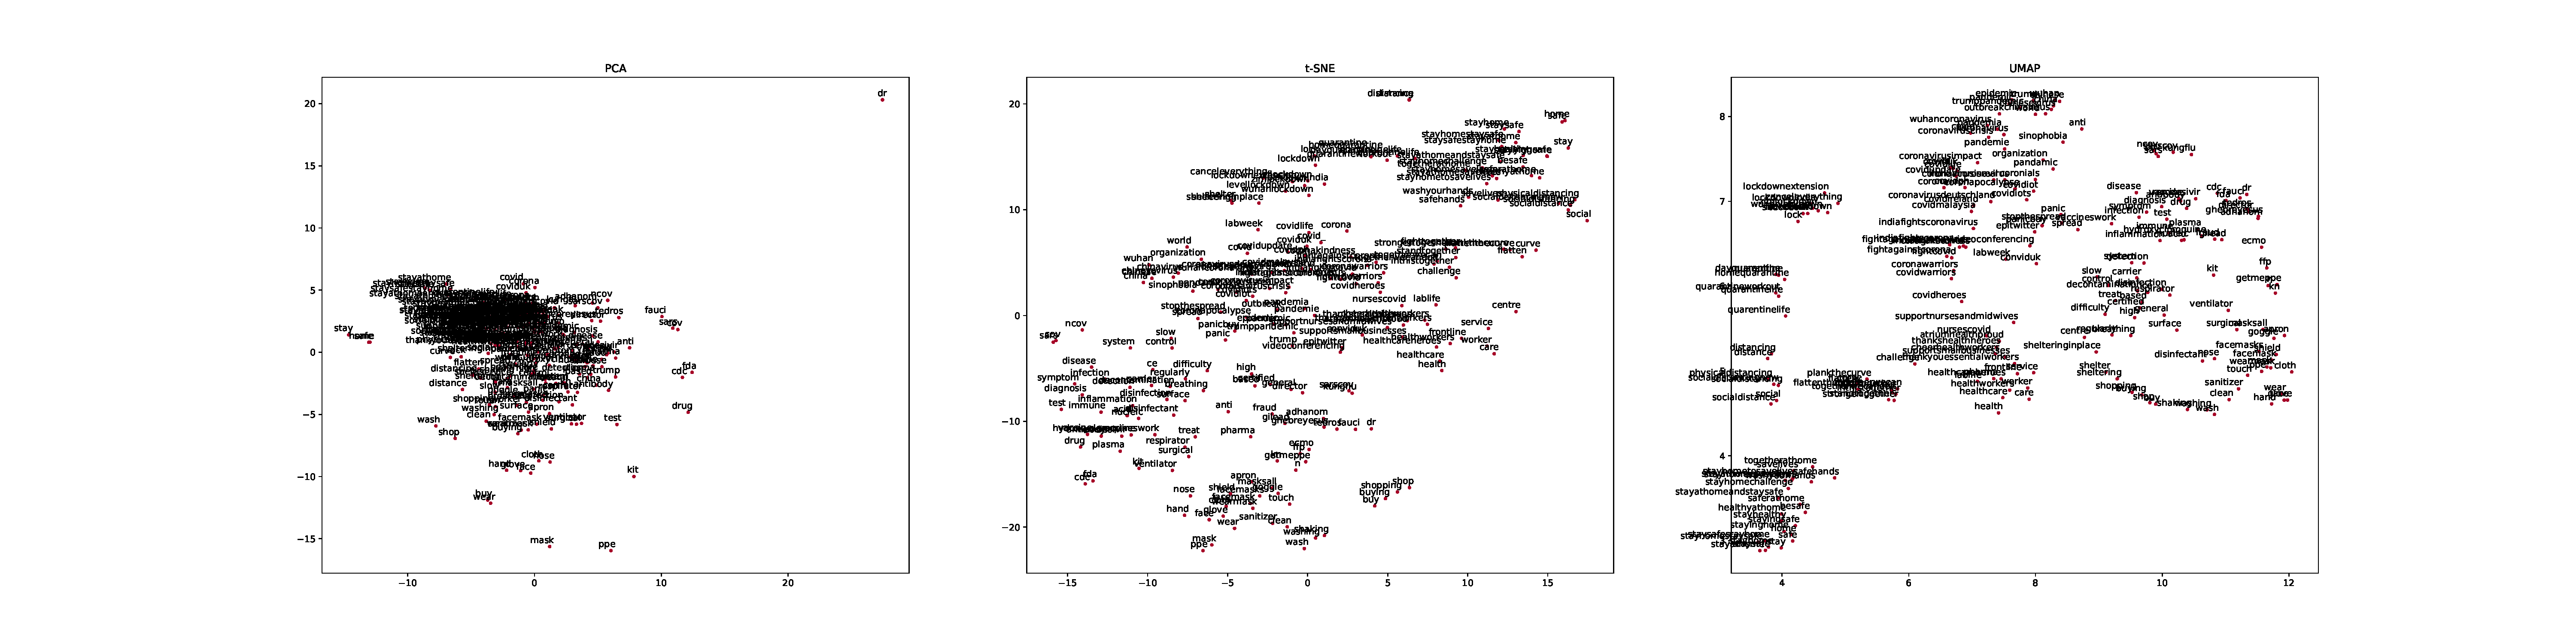
\includegraphics[width=1\textwidth]{images/keywords_ft.pdf}
 \caption{Distribution of keywords used to select tweets for the TweetsCOV19 dataset.}
 \label{fig:ft_key}
 \end{subfigure}
 \centering
 \begin{subfigure}{\columnwidth}
 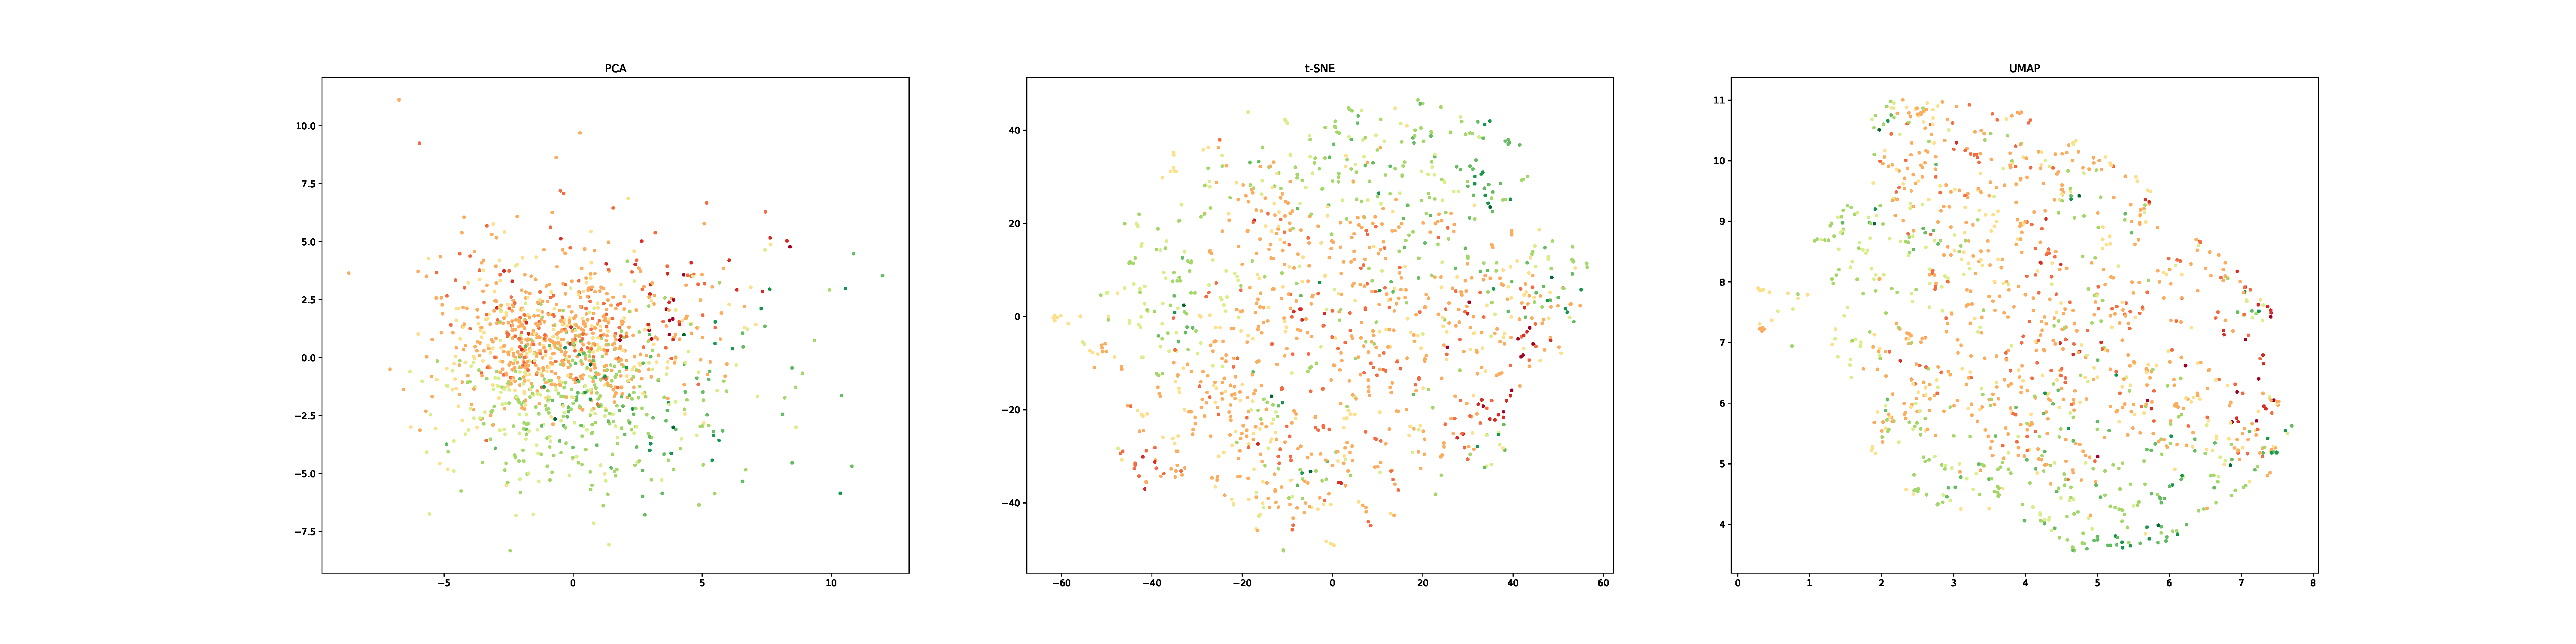
\includegraphics[width=1\textwidth]{images/keywords_ft_posneg.pdf}
 \caption{Distribution of positive and negative words from the AFINN-96 dataset.}
  \label{fig:ft_posneg}
 \end{subfigure}
 \caption{Visualization of FastText embedding of keywords and positive/negative words with PCA, t-SNE, and UMAP.}
 \label{fig:ft_viz}
\end{figure}

\begin{figure}
 \centering
 \begin{subfigure}{\columnwidth}
 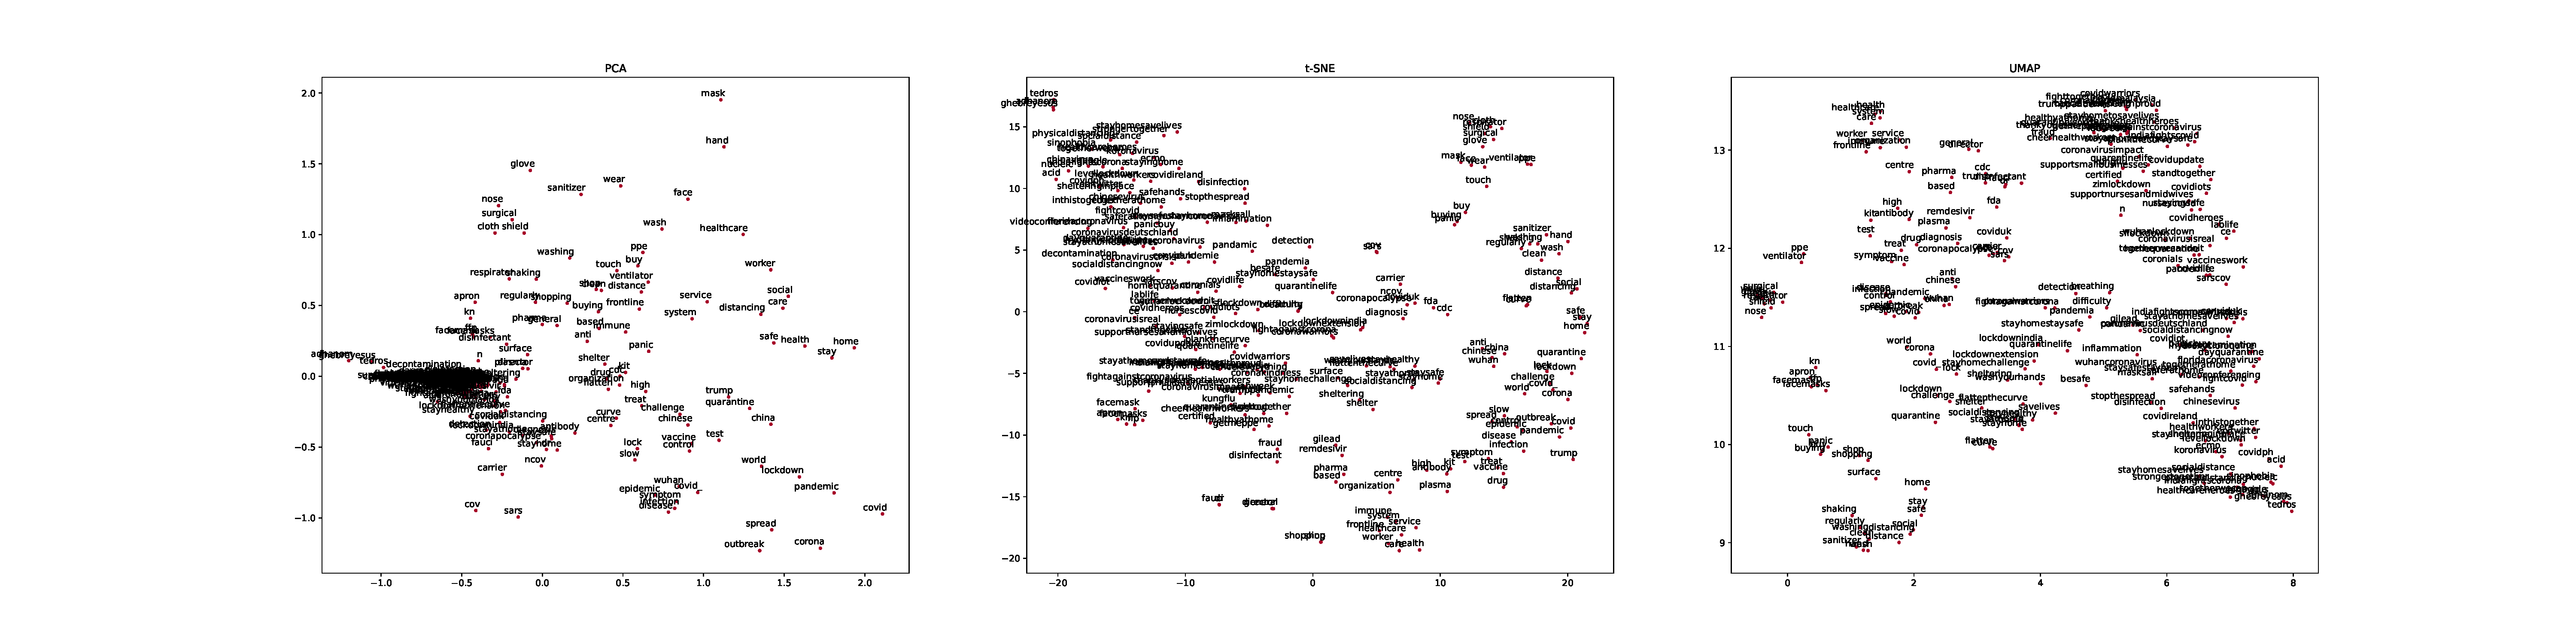
\includegraphics[width=1\textwidth]{images/keywords_glove.pdf}
 \caption{Distribution of keywords used to select tweets for the TweetsCOV19 dataset.}
 \label{fig:glove_key}
 \end{subfigure}
 \centering
 \begin{subfigure}{\columnwidth}
 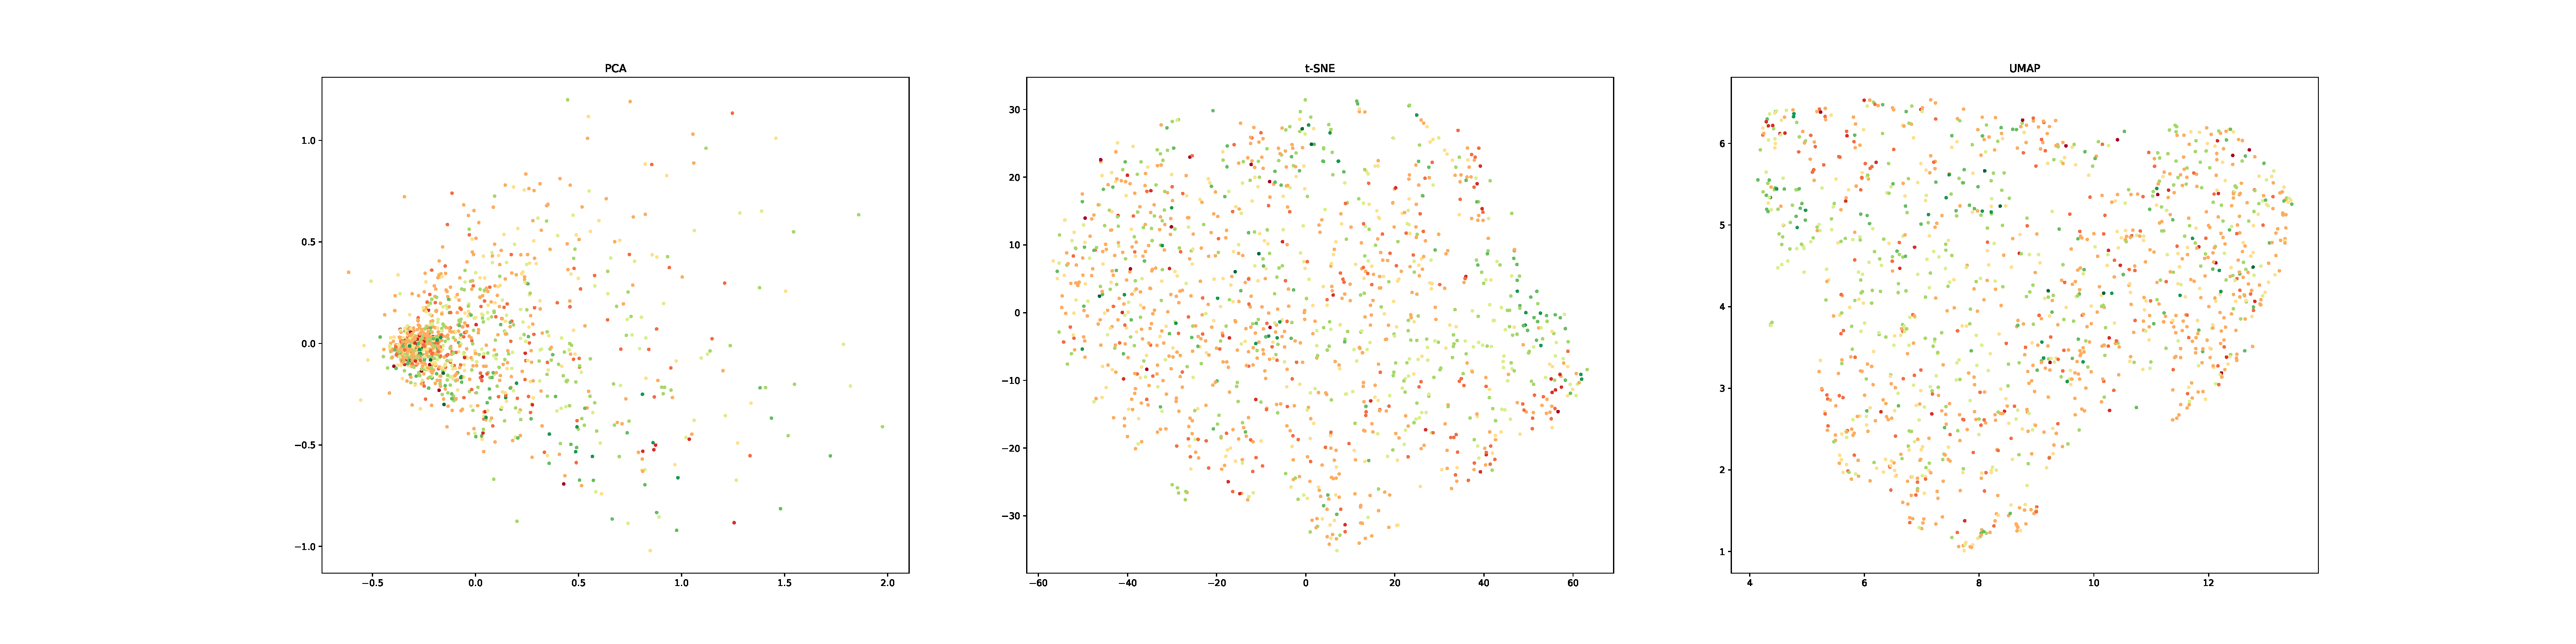
\includegraphics[width=1\textwidth]{images/keywords_glove_posneg.pdf}
 \caption{Distribution of positive and negative words from the AFINN-96 dataset.}
  \label{fig:glove_posneg}
 \end{subfigure}
 \caption{Visualization of Glove embedding of keywords and positive/negative words with PCA, t-SNE, and UMAP.}
 \label{fig:glove_viz}
\end{figure}

After embedding of keywords with FastText, we can see a clear grouping of similar words when visualized with t-SNE and especially UMAP, as can be seen in Figure \ref{fig:ft_key}. This makes sense, since FastTexts looks at the morphological similarity of words by working with n-grams. For example, in the UMAP visualization, 'distancing' and 'distance' are grouped together, but 'physicaldistancing', 'socialdistancing', and 'socialdistance' are also located nearby. This will likely make it easier for FastText to assign similar scores to similar words, e.g. to 'bad' and 'badly'.

Embeddings with GloVe, Skip-grams, and CBOW seem to capture more subtle relationships, and UMAP visualization is able to group words such as 'facemask', 'kn', and 'ffp' together. The visualizations can be found in Figures \ref{fig:glove_key}, \ref{fig:sgram_key}, and \ref{fig:cbow_key}. Classification results using any of these embedding models will therefore in all likelihood be relatively similar. 

Application of PCA on the embedding with CBOW, Skip-grams, and FastText seems to show a reasonable separation of positive and negative words, although the t-SNE and UMAP visualizations do not noticeably confirm this finding (see Figure \ref{fig:cbow_posneg}, \ref{fig:ft_posneg}, and \ref{fig:sgram_posneg}). GloVe embedding, on the other hand, seems to not be easily separable in two dimensions after application of PCA, but shows similar results for t-SNE and UMAP, as can be seen in Figure \ref{fig:glove_posneg}.
In general, we can see that most of embedding models are able to pick up on the sentiments of certain words, but not on the relative weights of that sentiment. Therefore, it might be difficult for our downstream classifiers to pick up on these nuances, and especially so when using GloVe embeddings.

\subsection*{Q7: Tweet embeddings (2 pts)}
\textit{Propose three different approaches to combine word embeddings into an embedding for each tweet. Provide a code snippet for each function. How do all of the above methods deal with out-of-vocabulary words?}

For this question, we compare summing, averaging, and concatenation of the minimum and maximum of the word embeddings.

Our 'summing' method simply consists of summing up the embeddings of every word in the tweet. If a word cannot be found in the vocabulary, we do not include it in the sum (this is done because we limited vocabulary size in some of our methods for computational reasons).

The 'averaging' method uses the results from the first 'summing' method, but divides it by the number of valid (i.e. not OOV) words found in the tweet.

The code for the first two methods can be found in Code Snippet \ref{listing:p2-sumav}.

\begin{listing*}
\begin{minted}{python}
def av_sum_sentence(row, model, vec_size=vec_size, av=True):
    if row != []:
        red = 0
        sentence = 0
        for word in row:
            try:
                sentence += model.wv[word]
            except:
                red += 1
        if av:
            sentence = sentence/(1+len(row)-red)
        if red == len(row):
            return np.zeros(vec_size).tolist()
        else:
            return sentence.tolist()
    else:
        return np.zeros(vec_size).tolist()


def av_sum_sentence_bow(row, vectorizer, transformer=None, av=True):
    sentence = vectorizer.transform([row])
    if transformer is not None:
        sentence = transformer.transform(sentence)
    sentence = sentence.toarray()[0]
    if av:
        sentence = sentence/(1+sentence.sum())
    return sentence.tolist()
\end{minted}
\caption{Code of our 'summing' and 'averaging' word-to-sentence embedding functions. We created two functions to account for the individual differences between Gensim \cite{gensim} and scikit-learn \cite{sklearn1, sklearn2}.}
\label{listing:p2-sumav}
\end{listing*}

Finally, we designed a 'minmax' method, where we find the respective minimum and maximum values (per index) of all word embeddings and concatenate the results. Again, as can be seen in Code Snippet \ref{listing:p2-minmax}, if a word is OOV, we simply ignore it.

\begin{listing*}
\begin{minted}{python}
def minmax_sentence(row, model, vec_size=vec_size):
    sentence_min = np.ones(vec_size)*1000
    sentence_max = np.ones(vec_size)*(-1000)
    if row != []:
        red = 0
        for word in row:
            try:
                sentence_min = np.minimum(np.asarray(model.wv[word]), sentence_min[idx])
                sentence_max = np.maximum(np.asarray(model.wv[word]), sentence_max[idx])
            except:
                red += 1
        if red == len(row):
            sentence_min = np.ones(vec_size)*1000
            sentence_max = np.ones(vec_size)*(-1000)
    return np.concatenate((sentence_min, sentence_max), axis=0).tolist()

def minmax_sentence_bow(row, vectorizer, vocab_size, transformer=None):
    sentence_min = np.ones(vocab_size)
    sentence_max = np.zeros(vocab_size)
    
    if row != []:
        res = vectorizer.transform([row])
        if transformer is not None:
            res = transformer.transform(res)
        sentence_min = np.minimum(res.toarray()[0], sentence_min)
        sentence_max = np.maximum(res.toarray()[0], sentence_max)
    return np.concatenate((sentence_min, sentence_max), axis=0).tolist()
\end{minted}
\caption{Code of our 'minmax' word-to-sentence embedding function. There are two functions, in order to account for the differences between the Gensim \cite{gensim} and scikit-learn libraries \cite{sklearn1, sklearn2}.}
\label{listing:p2-minmax}
\end{listing*}


\subsection*{Q8: Classifier (3 pts)}
\textit{Implement three downstream classifiers to perform sentiment analysis of your tweets (i.e., predict both the positive (1 to 5) and negative (-1 to -5) sentiment score for each tweet). For each classifier, briefly explain how it works and make sure to tune hyper-parameters appropriately. Provide a results table showcasing the performance of all tested classifiers for each embeddings approach you implemented in Q1-5, and each aggregation method in Q7. For each family of classifiers tested provide a code snippet.}

Instead of classifiers, we implement three regression models to perform sentiment analysis of the tweets, since the labels 'positive sentiment score' and 'negative sentiment score' are ordered discrete values. We compare our results using the mean harmonic F1 score (i.e. the mean of the harmonic F1 score for positive and negative sentiments respectively).

Before calculating the harmonic F1 score, we round the regression output to the nearest integer, and then clip all values outside of the sentiment score range (1 to 5 for positive sentiments, and -5 to -1 for negative sentiments), to ensure consistency with classifier outputs. This details of this preprocessing step can be found in Code Snippet \ref{listing:f1}

\begin{listing*}
\begin{minted}{python}
from sklearn.metrics import f1_score, make_scorer

def weighted_harmonic_f1_score(y_true, y_pred):
    y_pred_pos = np.clip(np.around(y_pred[:,0]), 1, 5).astype(int)
    y_pred_neg = np.clip(np.around(y_pred[:,1]), -5, -1).astype(int)
    f1_scores_pos = f1_score(y_true[:,0], y_pred_pos, average='weighted')
    f1_scores_neg = f1_score(y_true[:,1], y_pred_neg, average='weighted')
    weighted_f1 = (f1_scores_pos + f1_scores_neg)/2
    return weighted_f1

weighted_harmonic_f1_scorer = make_scorer(weighted_harmonic_f1_score)

\end{minted}
\caption{Code snippet showing the calculation of the weighted harmonic F1 score used in Q8.}
\label{listing:f1}
\end{listing*}


All hyperparameter tuning was performed using GridSearchCV from the scikit-learn library \cite{sklearn1, sklearn2}. Still, to speed up training, we tune the models with limited parameters and train on only two folds.

For our first 'classifier', we use Random Forests \cite{randomforest}. Random Forests is a model that combines the results of multiple decision trees, returning the most likely class for classification, or the mean prediction for regression. The code can be found in Code Snippet \ref{listing:p2-randomforest}.

\begin{listing*}
\begin{minted}{python}
from sklearn.ensemble import RandomForestRegressor
from sklearn.model_selection import GridSearchCV
from sklearn.multioutput import MultiOutputRegressor


def rand_forest(sentence, sentence_test):
    params = {'estimator__n_estimators':[5,15],
              'estimator__n_jobs':[-1], 'estimator__random_state':[42],
              'estimator__criterion':['squared_error'], 'estimator__max_depth':[4,5],
              'estimator__verbose':[0]}
    regr = GridSearchCV(MultiOutputRegressor(RandomForestRegressor()), param_grid=params,
                        n_jobs=-1, cv=2, scoring=weighted_harmonic_f1_scorer, verbose=0)
    start_time = time.time()
    regr.fit(sentence, np.asarray(y_train_val[['pos_sent', 'neg_sent']].values.tolist()))
    elapsed_time = time.time() - start_time

\end{minted}
\caption{Code snippet for the first classifier, Random Forests.}
\label{listing:p2-randomforest}
\end{listing*}

For the second 'classifier', we use GradientBoosting \cite{gradboost1, gradboost2, gradboost3}. Gradient boosting is a method that combines weak models to create a strong predictive model. It does so by iteratively improving upon the loss from the weak model of the previous round.
We again use a method from scikit-learn \cite{sklearn1, sklearn2}, as you can see in \ref{listing:p2-gradboost}.

\begin{listing*}
\begin{minted}{python}
from sklearn.ensemble import GradientBoostingRegressor

def grad_reg(sentence, sentence_test):
    params = {'estimator__learning_rate': [0.1, 1], 'estimator__n_estimators': [5, 15],
              'estimator__max_depth': [4, 5], 'estimator__n_iter_no_change':[7]}
    regr = GridSearchCV(MultiOutputRegressor(GradientBoostingRegressor()), param_grid=params,
                        n_jobs=-1, cv=2, scoring=weighted_harmonic_f1_scorer, verbose=0)
    start_time = time.time()
    regr.fit(sentence, np.asarray(y_train_val[['pos_sent', 'neg_sent']].values.tolist()))
    elapsed_time = time.time() - start_time
\end{minted}
\caption{Code snippet for the second classifier, Gradient Boosting.}
\label{listing:p2-gradboost}
\end{listing*}

Finally, for our third 'classifier', we implemented AdaBoost \cite{adaboost} in Code Snippet \ref{listing:p2-adaboost}. Adaptive boosting is an iterative training method that in every iteration adjusts the weights of  the data points that were predicted badly in the previous iteration. The final output is the weighted average of all previous models, the weights depending on their overall performance.

\begin{listing*}
\begin{minted}{python}
from sklearn.ensemble import AdaBoostRegressor

def ada_reg(sentence, sentence_test):
    params = {'estimator__loss': ['square', 'exponential'], 'estimator__n_estimators': [5, 15, 30],
              'estimator__learning_rate': [0.1, 1, 10], 'estimator__random_state':[42]}
    regr = GridSearchCV(MultiOutputRegressor(AdaBoostRegressor()), param_grid=params,
                        n_jobs=-1, cv=2, scoring=weighted_harmonic_f1_scorer, verbose=0)
    start_time = time.time()
    regr.fit(sentence, np.asarray(y_train_val[['pos_sent', 'neg_sent']].values.tolist()))
    elapsed_time = time.time() - start_time
\end{minted}
\caption{Code snippet for the third classifier, AdaBoost.}
\label{listing:p2-adaboost}
\end{listing*}

The train and test scores of the classifiers for each word embedding model and aggregation method can be found in Table \ref{table:score}. 

\subsection*{Q9: Performance comparison (3 pts)}
\textit{Using the summary table computed in Q8, compare the performance of all methods on the sentiment analysis task using the TweetsCOV19 dataset. Also compare methods from a computational point of view. What embedding model, aggregation method and classifier would you select among all approaches? Give potential extensions that could help improve your performance.}

\begin{table}[]
\resizebox{\textwidth}{!}{%
\begin{tabular}{|l|lll|l|l|lll|}
\cline{1-4} \cline{6-9}
\textbf{TRAIN SCORE} & RandomForests & GradientBoosting & AdaBoost &  & \textbf{TEST SCORE} & RandomForests & GradientBoosting & AdaBoost \\ \cline{1-4} \cline{6-9} 
CBOW average & 0.48 & 0.54 & 0.48 &  & CBOW average & 0.48 & 0.53 & 0.48 \\
CBOW summing & 0.52 & 0.56 & 0.5 &  & CBOW summing & 0.52 & 0.56 & 0.5 \\
CBOW minmax & 0.08 & 0.08 & 0.48 &  & CBOW minmax & 0.08 & 0.08 & 0.48 \\ \cline{1-4} \cline{6-9} 
Skip-Grams average & 0.49 & 0.55 & 0.48 &  & Skip-Grams average & 0.49 & 0.54 & 0.47 \\
Skip-Grams summing & 0.51 & 0.56 & 0.51 &  & Skip-Grams summing & 0.51 & 0.55 & 0.51 \\
Skip-Grams minmax & 0.08 & 0.08 & 0.48 &  & Skip-Grams minmax & 0.08 & 0.08 & 0.48 \\ \cline{1-4} \cline{6-9} 
FastText average & 0.47 & 0.54 & 0.48 &  & FastText average & 0.47 & 0.53 & 0.48 \\
FastText summing & 0.52 & 0.56 & 0.49 &  & FastText summing & 0.52 & 0.55 & 0.49 \\
FastText minmax & 0.08 & 0.08 & 0.48 &  & FastText minmax & 0.08 & 0.08 & 0.48 \\ \cline{1-4} \cline{6-9} 
GloVe average & 0.08 & 0.08 & 0.48 &  & GloVe average & 0.08 & 0.08 & 0.48 \\
GloVe summing & 0.08 & 0.08 & 0.48 &  & GloVe summing & 0.08 & 0.08 & 0.48 \\
GloVe minmax & 0.08 & 0.08 & 0.48 &  & GloVe minmax & 0.08 & 0.08 & 0.48 \\ \cline{1-4} \cline{6-9} 
BoW average & 0.32 & 0.65 & 0.25 &  & BoW average & 0.32 & 0.65 & 0.25 \\
BoW summing & 0.32 & 0.65 & 0.48 &  & BoW summing & 0.32 & 0.65 & 0.48 \\
BoW minmax & 0.32 & 0.64 & 0.48 &  & BoW minmax & 0.32 & 0.64 & 0.48 \\ \cline{1-4} \cline{6-9} 
TF-IDF average & 0.32 & 0.65 & 0.48 &  & TF-IDF average & 0.32 & 0.65 & 0.48 \\
TF-IDF summing & 0.32 & 0.65 & 0.5 &  & TF-IDF summing & 0.32 & 0.65 & 0.5 \\
TF-IDF minmax & 0.32 & 0.65 & 0.48 &  & TF-IDF minmax & 0.32 & 0.65 & 0.48 \\ \cline{1-4} \cline{6-9} 
\end{tabular}%
}
\caption{Training and test results of all classifiers. The scoring was performed using the weighted harmonic F1 score.}
\label{table:score}
\end{table}

\begin{table}[]
\centering
\begin{tabular}{|l|lll|}
\hline
\textbf{EXECUTION TIME} & RandomForests & GradientBoosting & AdaBoost \\ \hline
CBOW average & 22.63 & 189.48 & 15.94 \\
CBOW summing & 34.42 & 188.15 & 18.28 \\
CBOW minmax & 3.42 & 232.97 & 228.01 \\ \hline
Skip-Grams average & 34.16 & 186.13 & 20.1 \\
Skip-Grams summing & 16.32 & 178.82 & 18.34 \\
Skip-Grams minmax & 3.05 & 7.09 & 7.68 \\ \hline
FastText average & 271.31 & 179.63 & 13.47 \\
FastText summing & 32.63 & 178.91 & 21.94 \\
FastText minmax & 3.06 & 4.42 & 6.2 \\ \hline
GloVe average & 2.2 & 2.48 & 236.42 \\
GloVe summing & 1.9 & 3.62 & 4.33 \\
GloVe minmax & 3.76 & 225.92 & 223.53 \\ \hline
BoW average & 45.85 & 66.99 & 78.58 \\
BoW summing & 248.67 & 59.41 & 47.88 \\
BoW minmax & 96.62 & 196.91 & 120.23 \\ \hline
TF-IDF average & 61.06 & 106.1 & 54.52 \\
TF-IDF summing & 57.18 & 115.27 & 83.28 \\
TF-IDF minmax & 102.66 & 234.46 & 118.18 \\ \hline
\end{tabular}
\caption{Execution time of the best model found with GridSearchCV for all classifiers, measured in seconds.}
\label{table:execution_time}
\end{table}

As can be seen in Table \ref{table:execution_time}, the execution time varies a lot, and is difficult to compare between classifiers and embedding/aggregator models due to external interference and computer usage. Still, in general, it seems like using the 'minmax' aggregator greatly increases training time, likely due to the increased size of the feature vectors.

In addition, when looking at the weighted harmonic F1 score (Table \ref{table:score}, the 'summing' aggregator seems to produce the best results when comparing aggregator models within each embedding model. Similarly, our GradientBoosting 'classifier', generally outperformed other classifier models with the same aggregator method and embedding model. The only exceptions were first of all the GloVe models, which ended up producing better results when trained with AdaBoost, but secondly also the 'minmax' aggregator, which produced better results (for the Gensim-based models) when trained with AdaBoost.

Somewhat suprising is the good results that were obtained using the simplest embedding methods: BoW and TF-IDF. This might be partially caused by the limitation of the vocabulary size, which affected the aggregator models differently than the Gensim-based models and also allowed the classifier to focus on the most frequently occurring words.

\begin{figure*}
    \centering
    \begin{subfigure}[b]{0.475\textwidth}
        \centering
        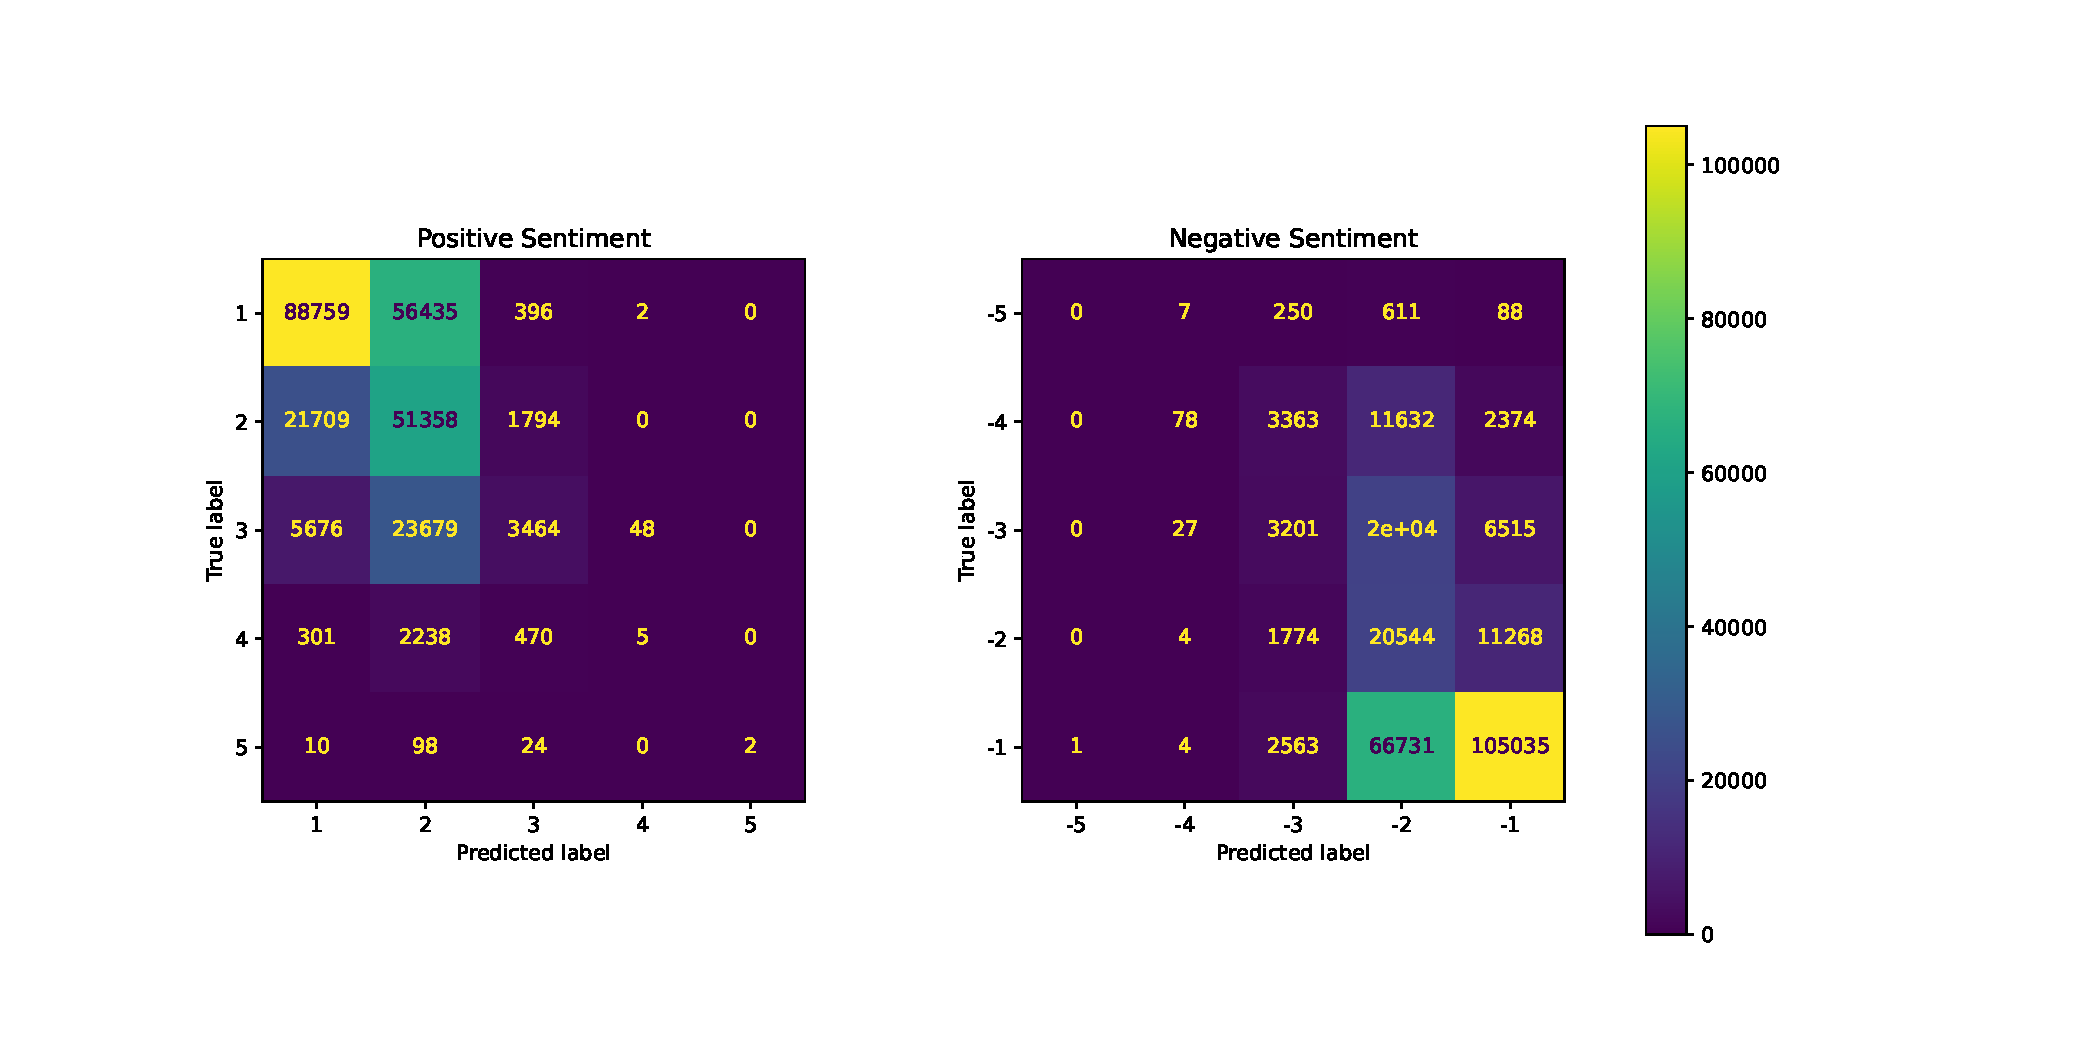
\includegraphics[width=\textwidth]{images/grad_boost_av_cbow.pdf}
        \caption{Confusion matrix for the Gradient Boosting 'classifier' trained on CBOW-embeddings that were aggregated by averaging.}    
        \label{fig:grad_boost_av_cbow}
    \end{subfigure}
    \hfill
    \begin{subfigure}[b]{0.475\textwidth}
        \centering
        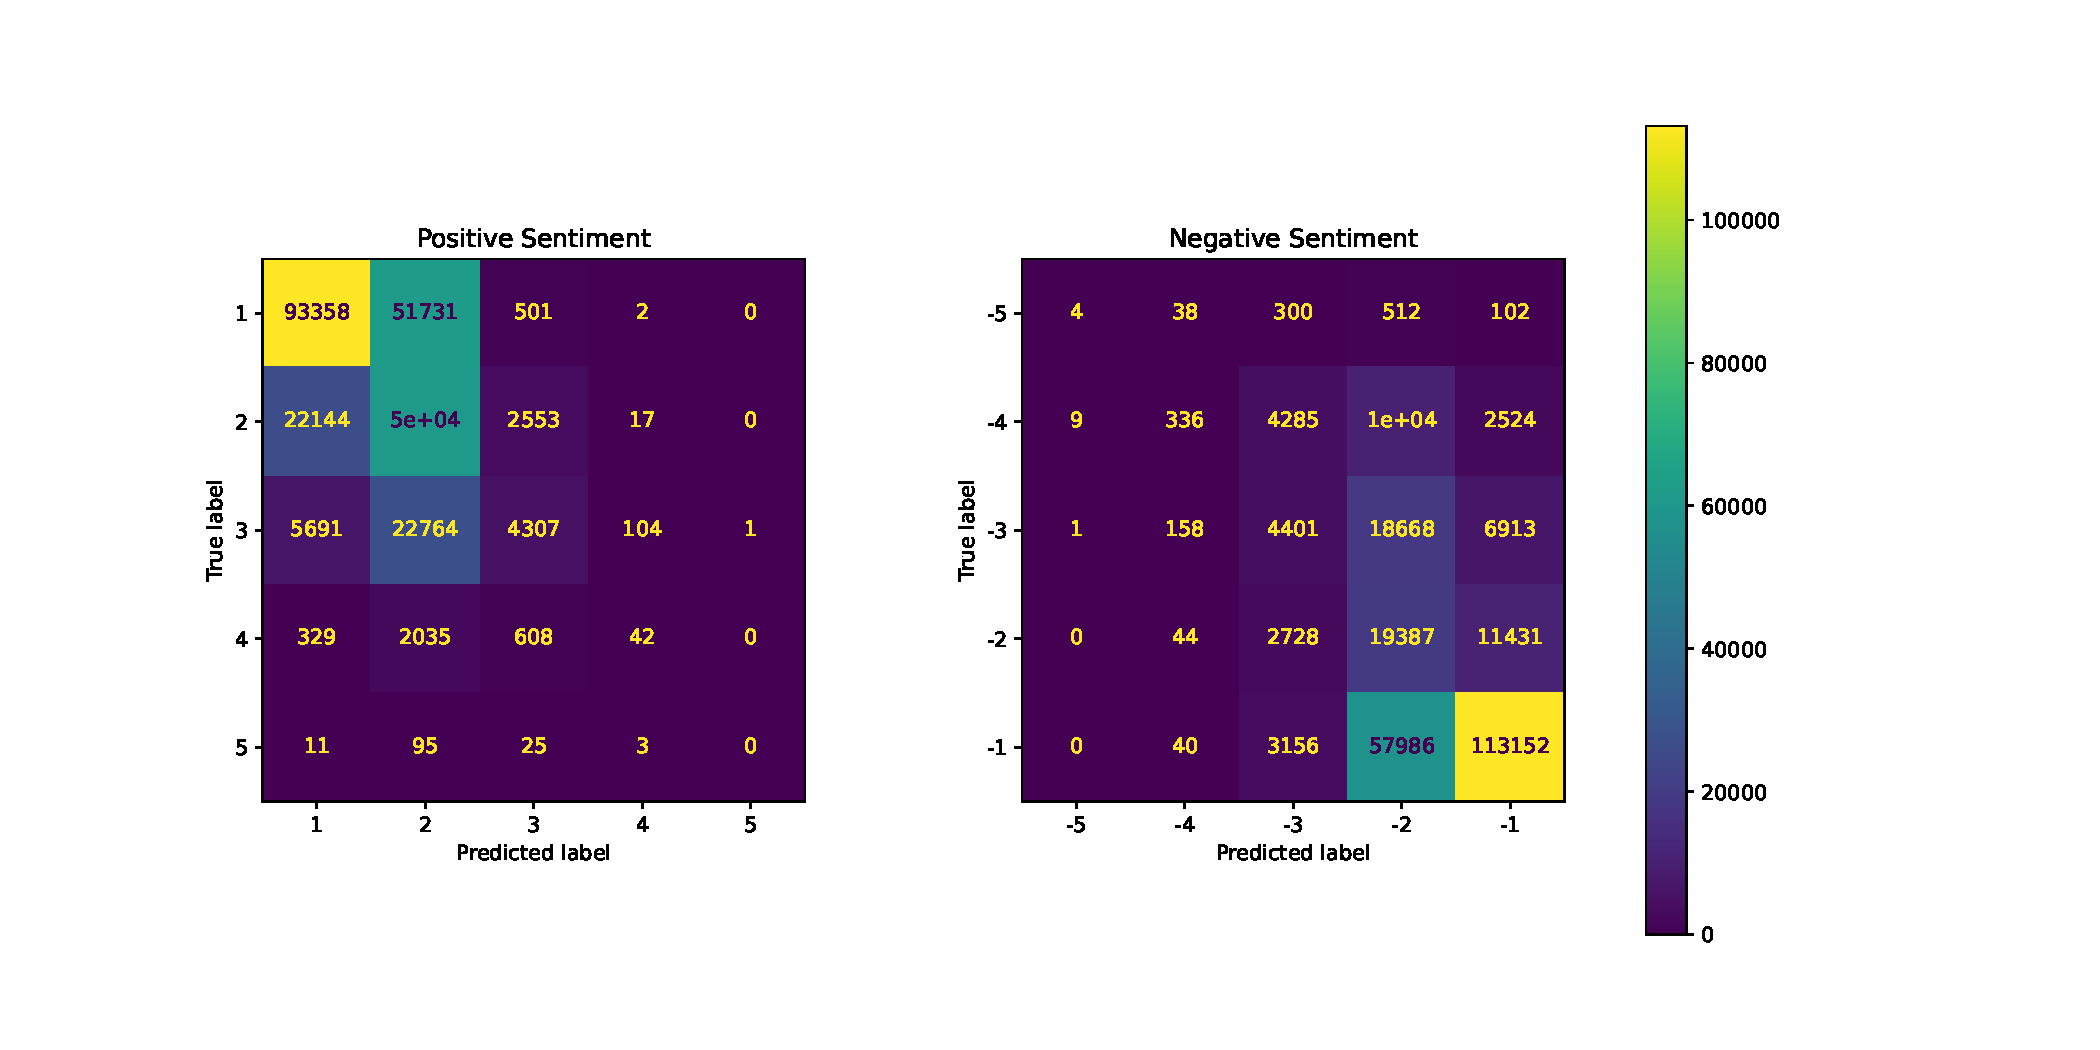
\includegraphics[width=\textwidth]{images/grad_boost_sum_cbow.pdf}
        \caption{Confusion matrix for the Gradient Boosting 'classifier' trained on CBOW-embeddings that were aggregated by summing.}    
        \label{fig:grad_boost_sum_cbow}
    \end{subfigure}
    \vskip\baselineskip
    \begin{subfigure}[b]{0.475\textwidth}
        \centering
        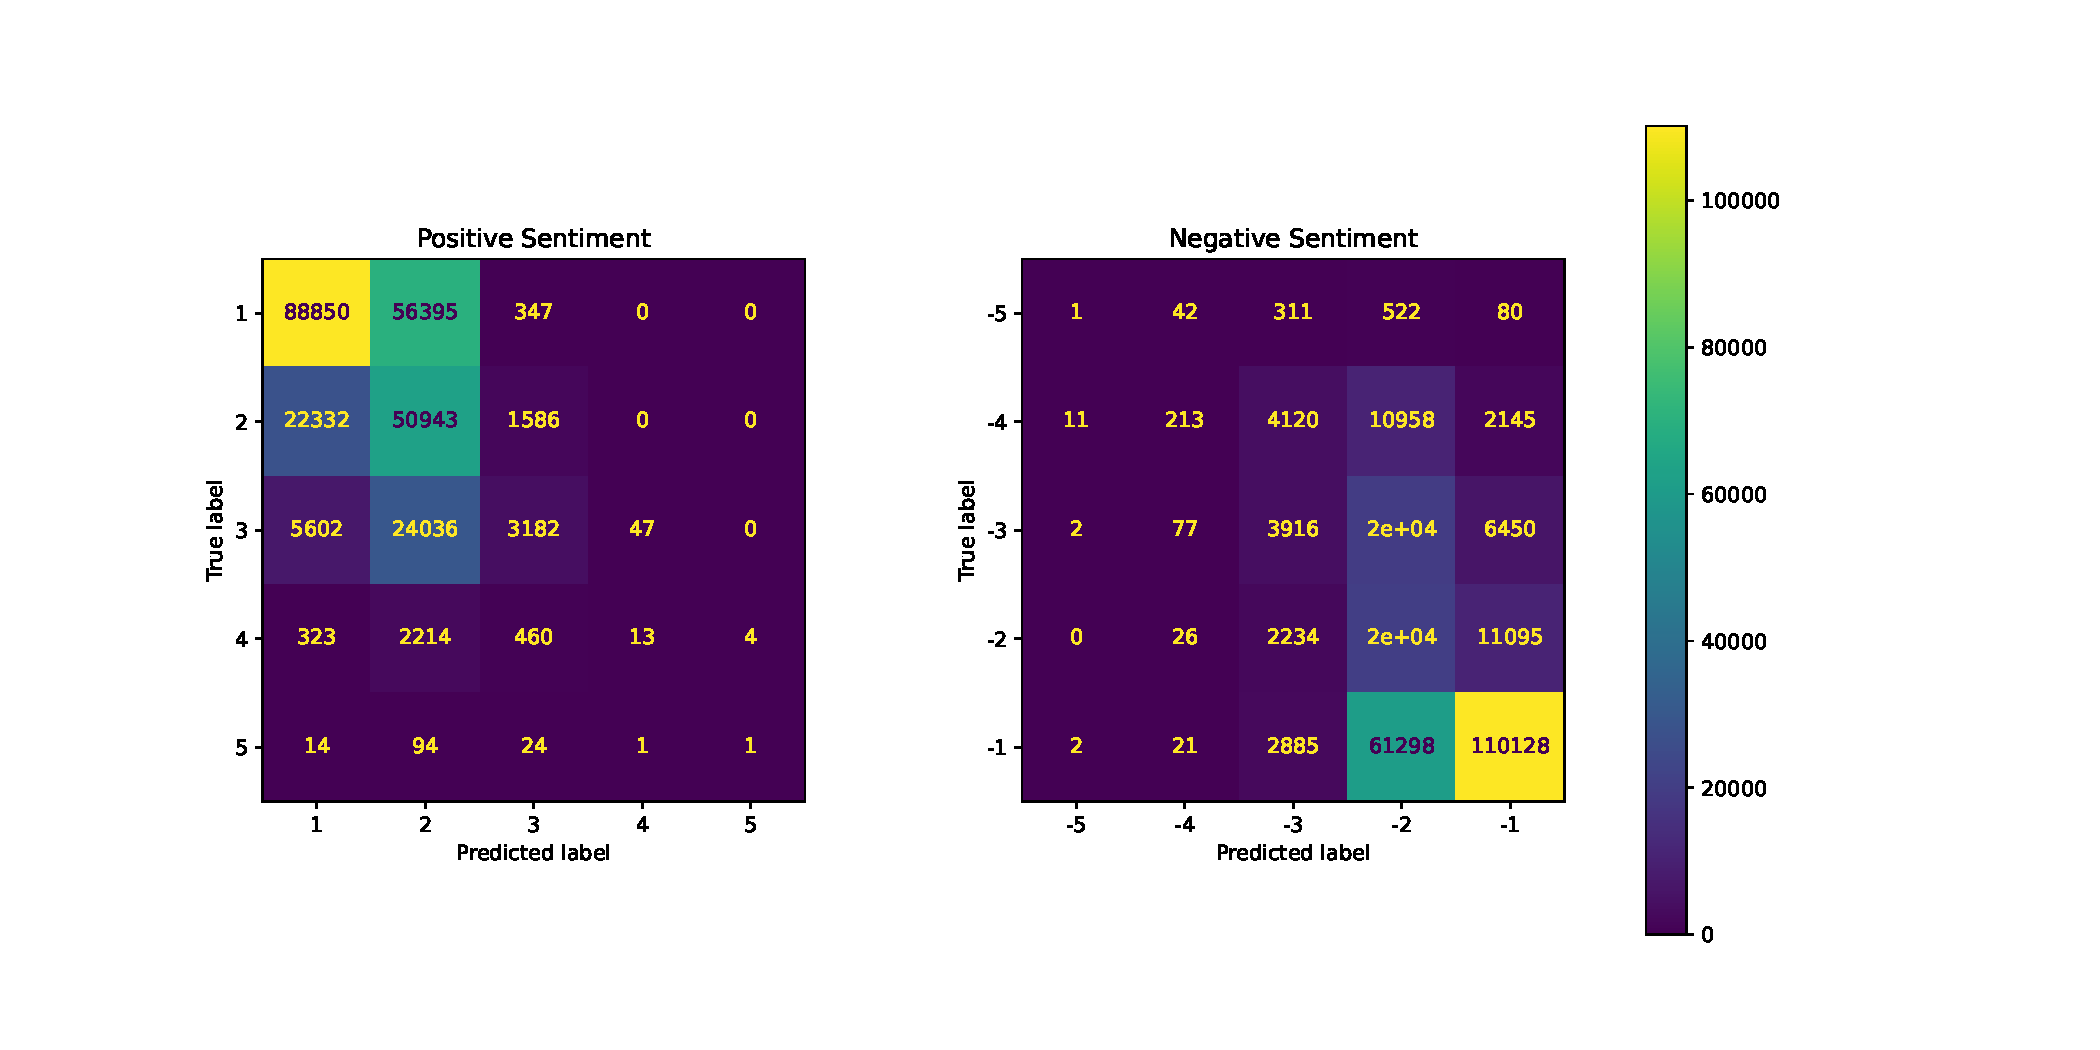
\includegraphics[width=\textwidth]{images/grad_boost_av_sgram.pdf}
        \caption{Confusion matrix for the Gradient Boosting 'classifier' trained on Skip-gram embeddings that were aggregated by averaging.}    
        \label{fig:grad_boost_av_sgram}
    \end{subfigure}
    \hfill
    \begin{subfigure}[b]{0.475\textwidth}
        \centering
        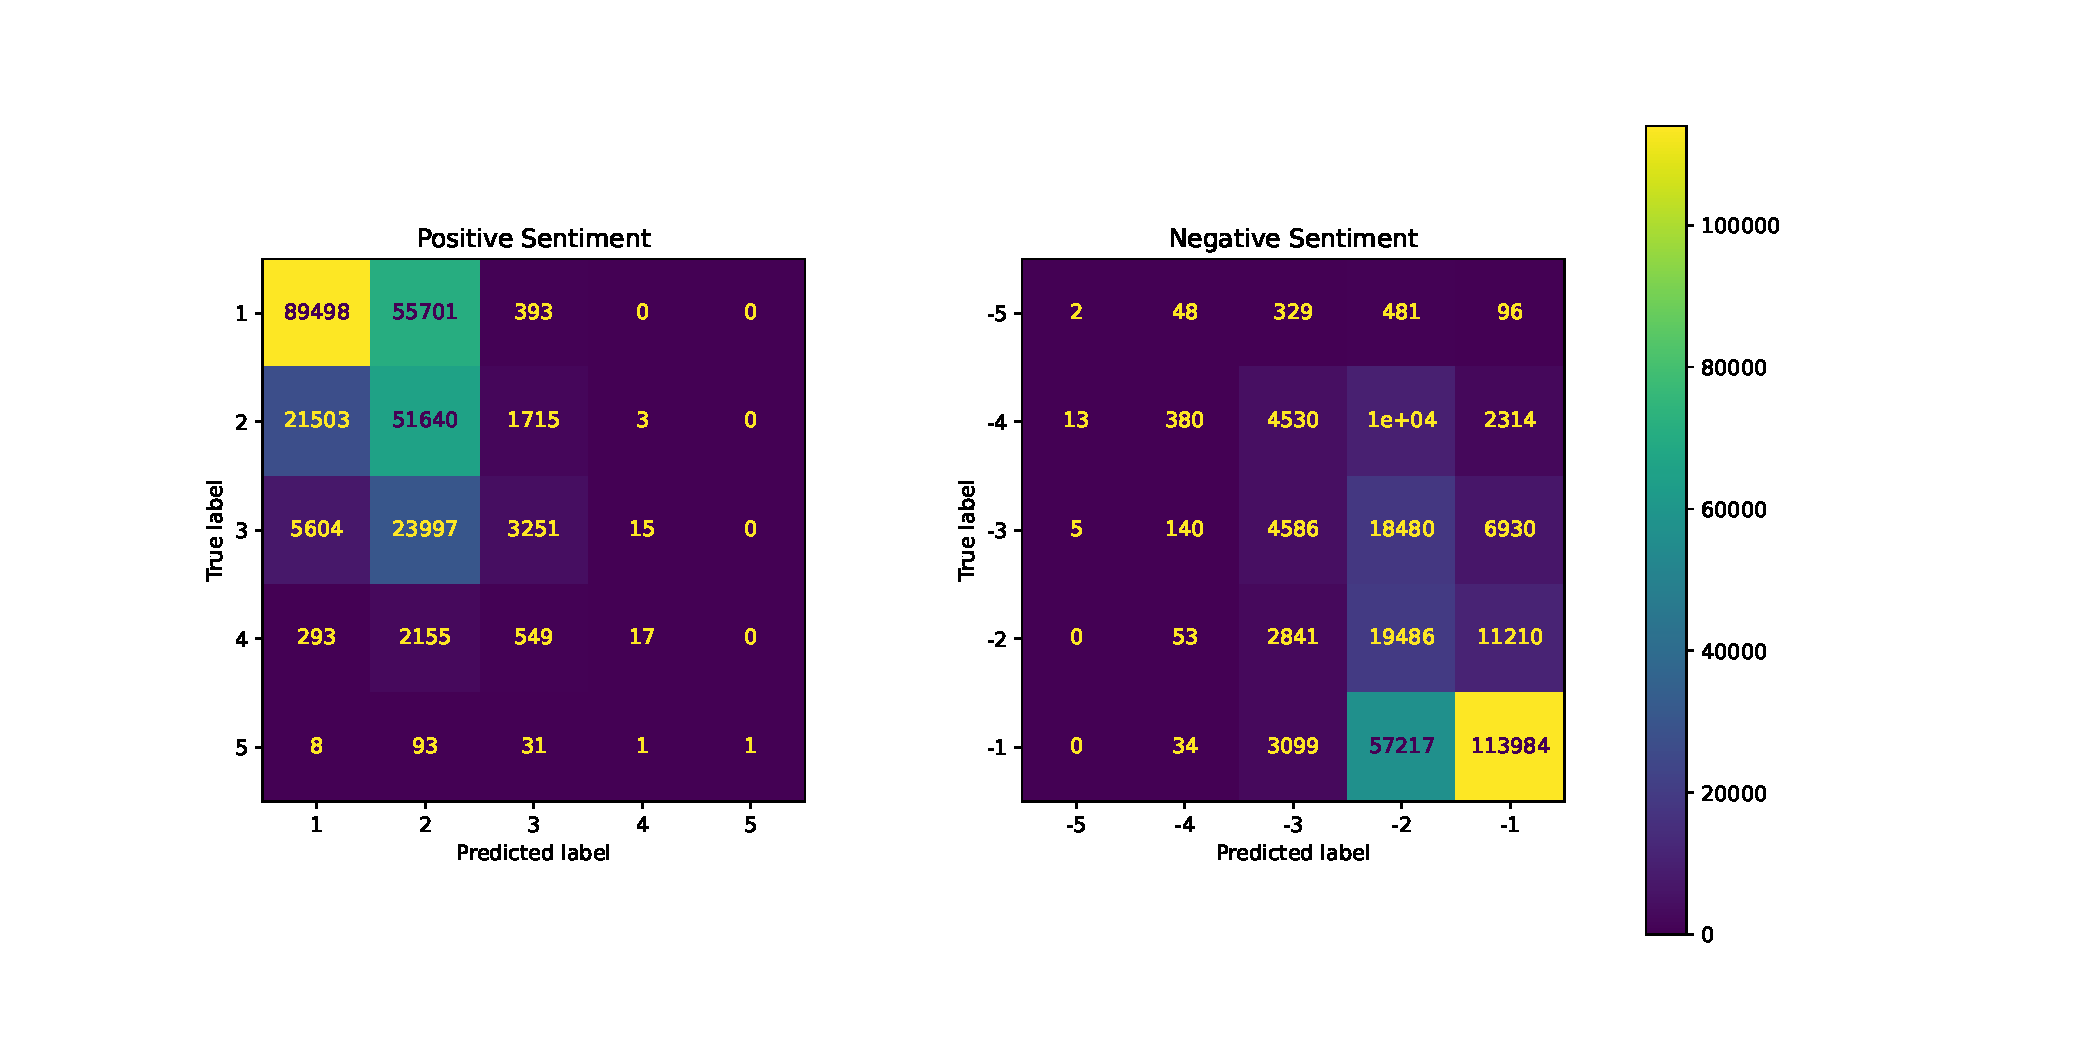
\includegraphics[width=\textwidth]{images/grad_boost_sum_sgram.pdf}
        \caption{Confusion matrix for the Gradient Boosting 'classifier' trained on Skip-gram embeddings that were aggregated by summing.}    
        \label{fig:grad_boost_sum_sgram}
    \end{subfigure}
   \vskip\baselineskip
    \begin{subfigure}[b]{0.475\textwidth}
        \centering
        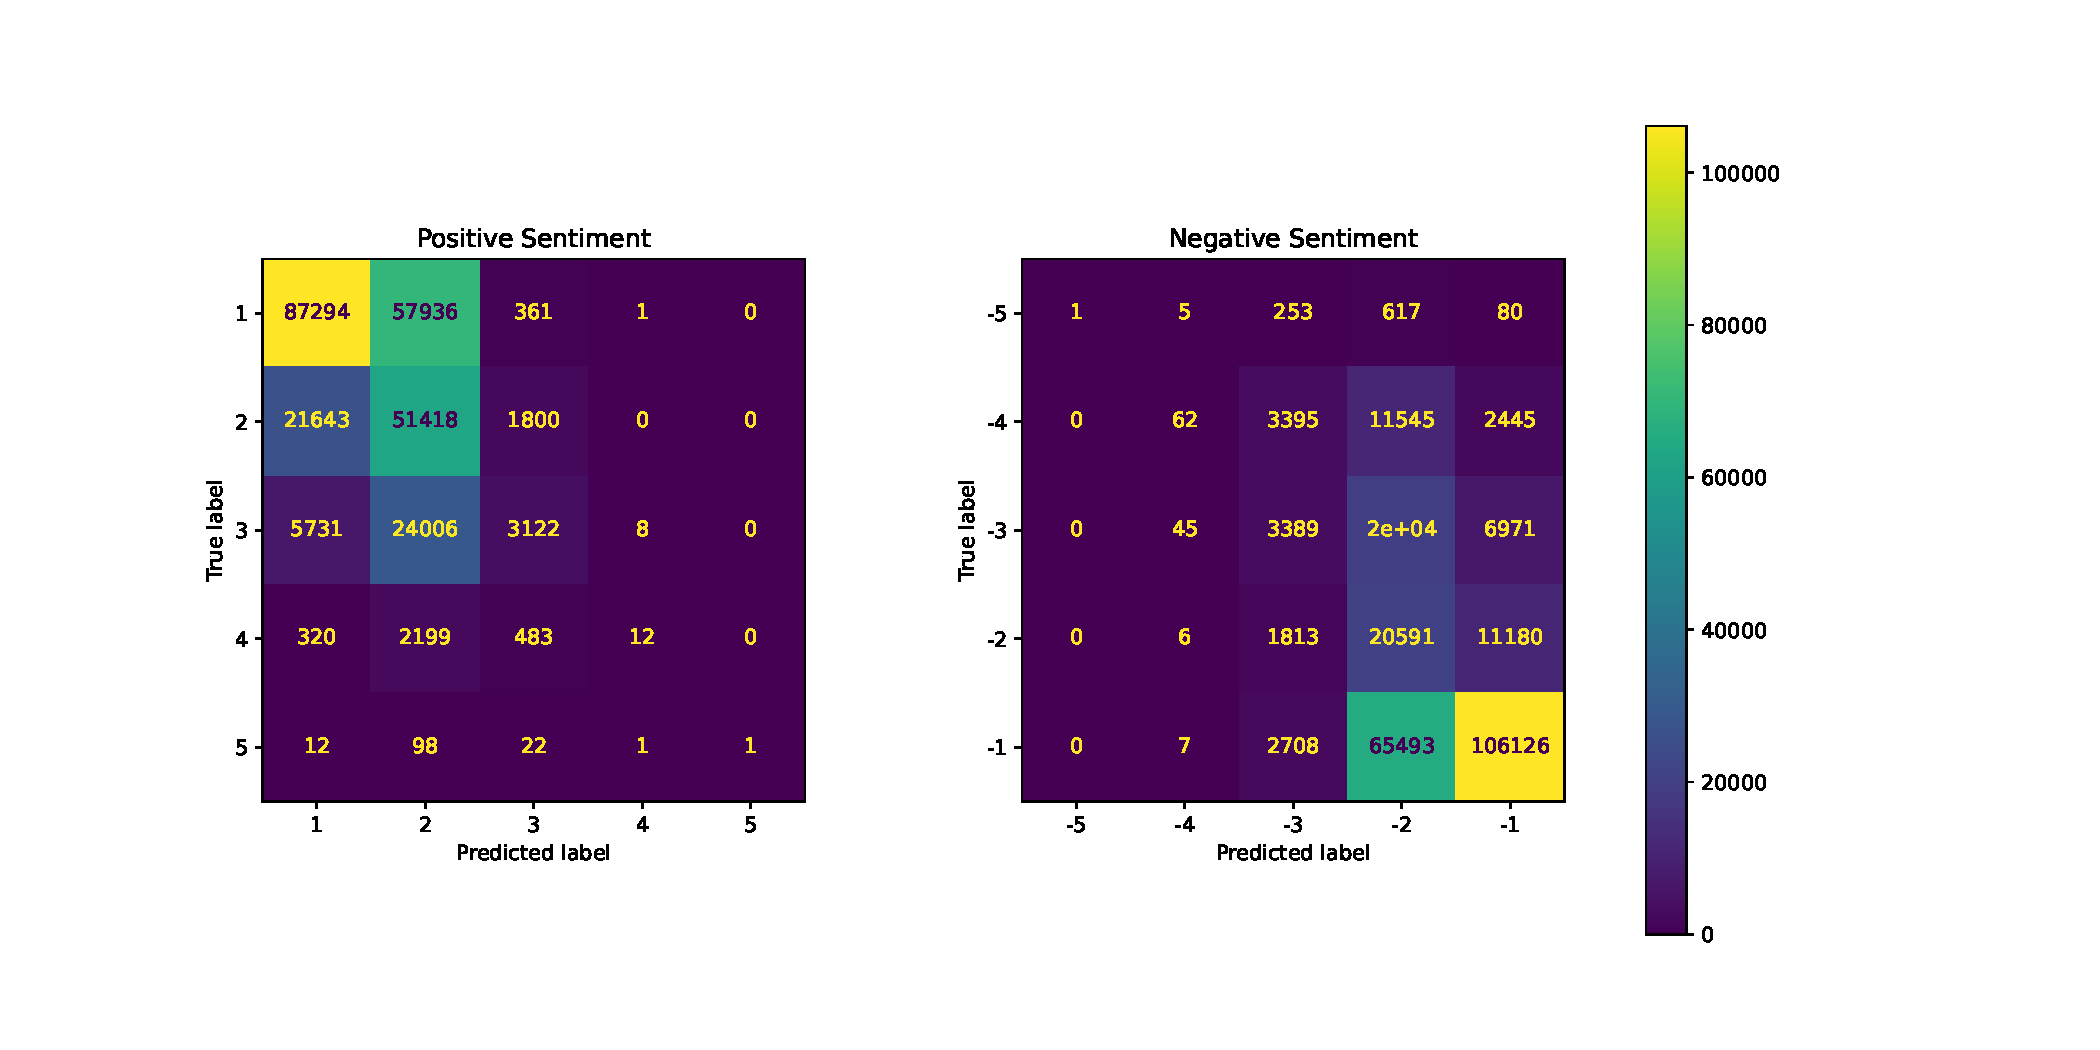
\includegraphics[width=\textwidth]{images/grad_boost_av_ft.pdf}
        \caption{Confusion matrix for the Gradient Boosting 'classifier' trained on FastText embeddings that were aggregated by averaging.}    
        \label{fig:grad_boost_av_ft}
    \end{subfigure}
    \hfill
    \begin{subfigure}[b]{0.475\textwidth}
        \centering
        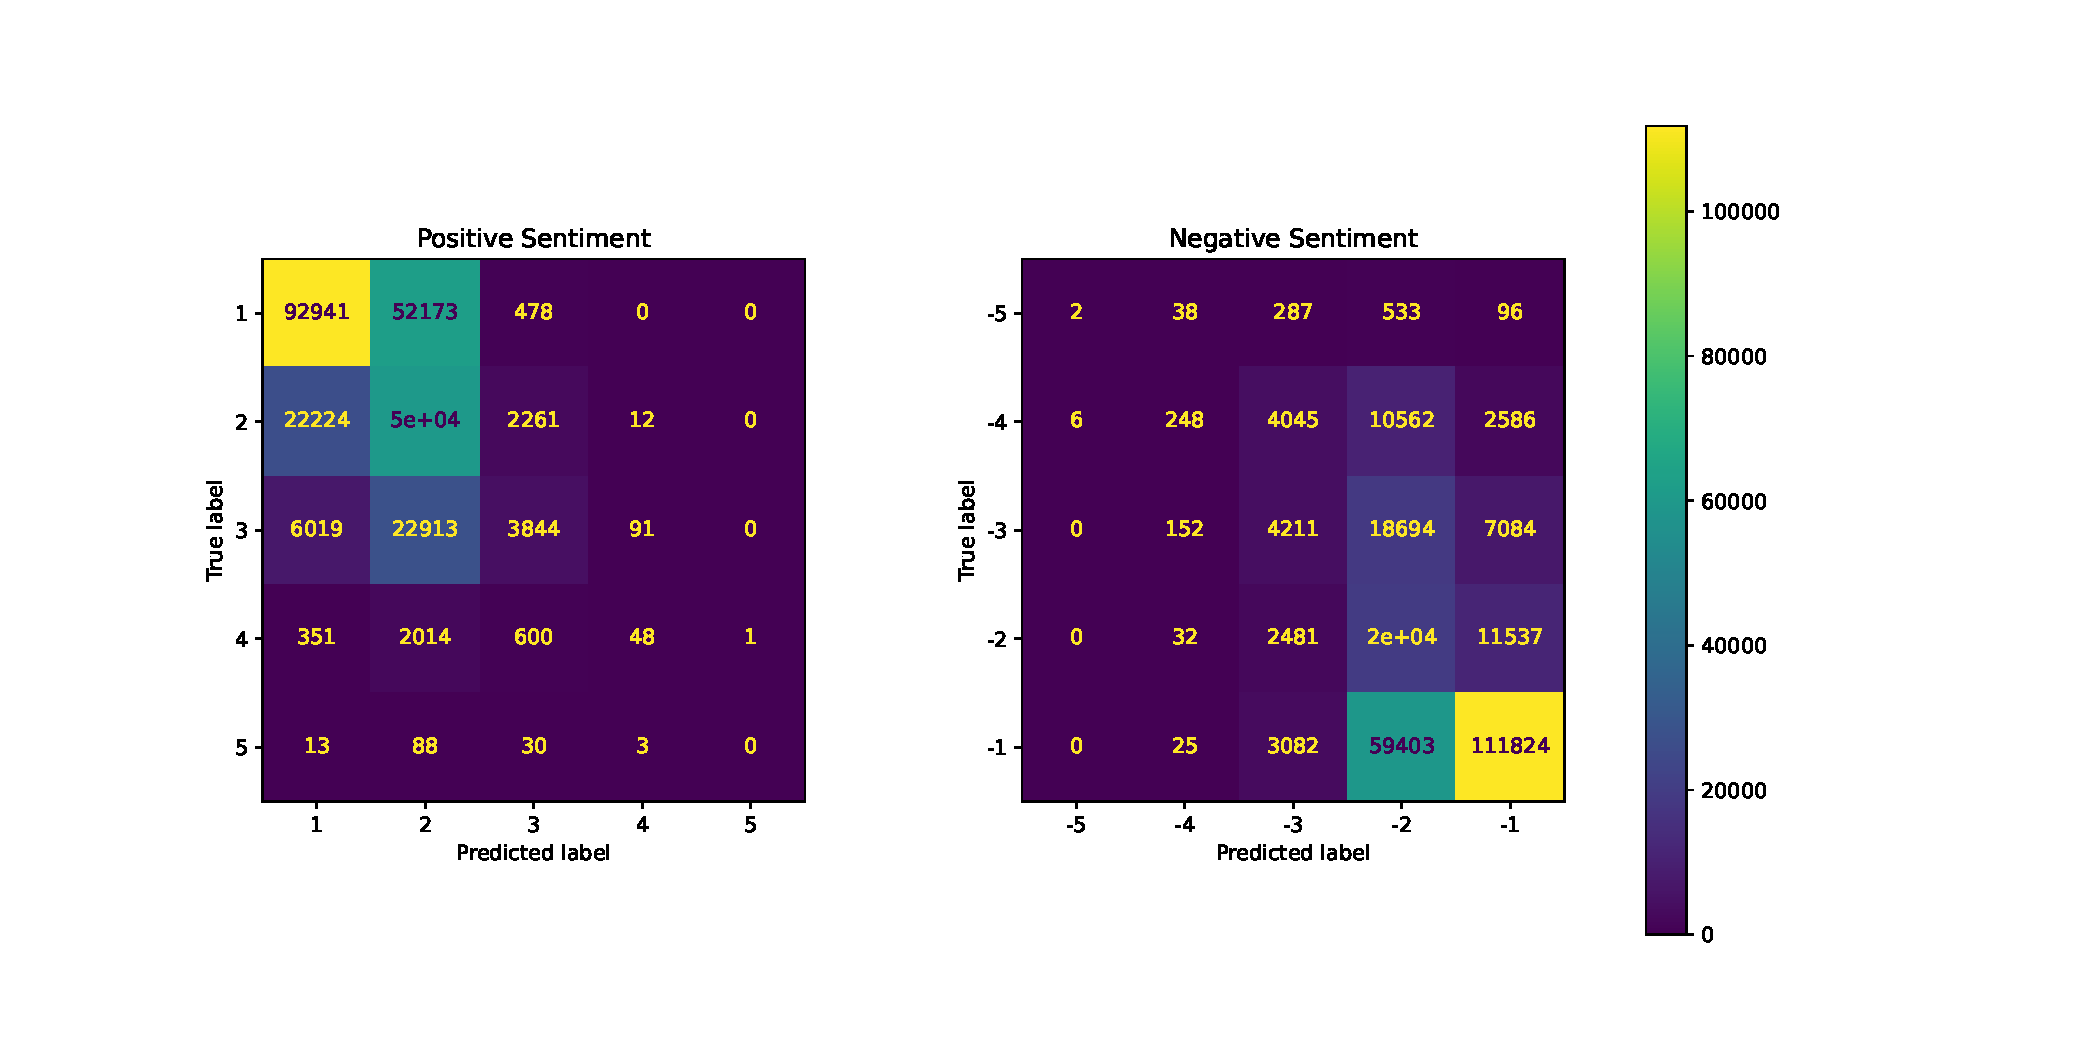
\includegraphics[width=\textwidth]{images/grad_boost_sum_ft.pdf}
        \caption{Confusion matrix for the Gradient Boosting 'classifier' trained on FastText embeddings that were aggregated by summing.}    
        \label{fig:grad_boost_sum_ft}
    \end{subfigure}
    \caption{Confusion matrices of six models trained with the Gradient Boosting algorithm. The models were selected based on a cutoff of $\ge 0.54$ for the training score (weighted harmonic F1 score).} 
    \label{fig:confusion_gensim}
\end{figure*}


\begin{figure*}
    \centering
    \begin{subfigure}[b]{0.475\textwidth}
        \centering
        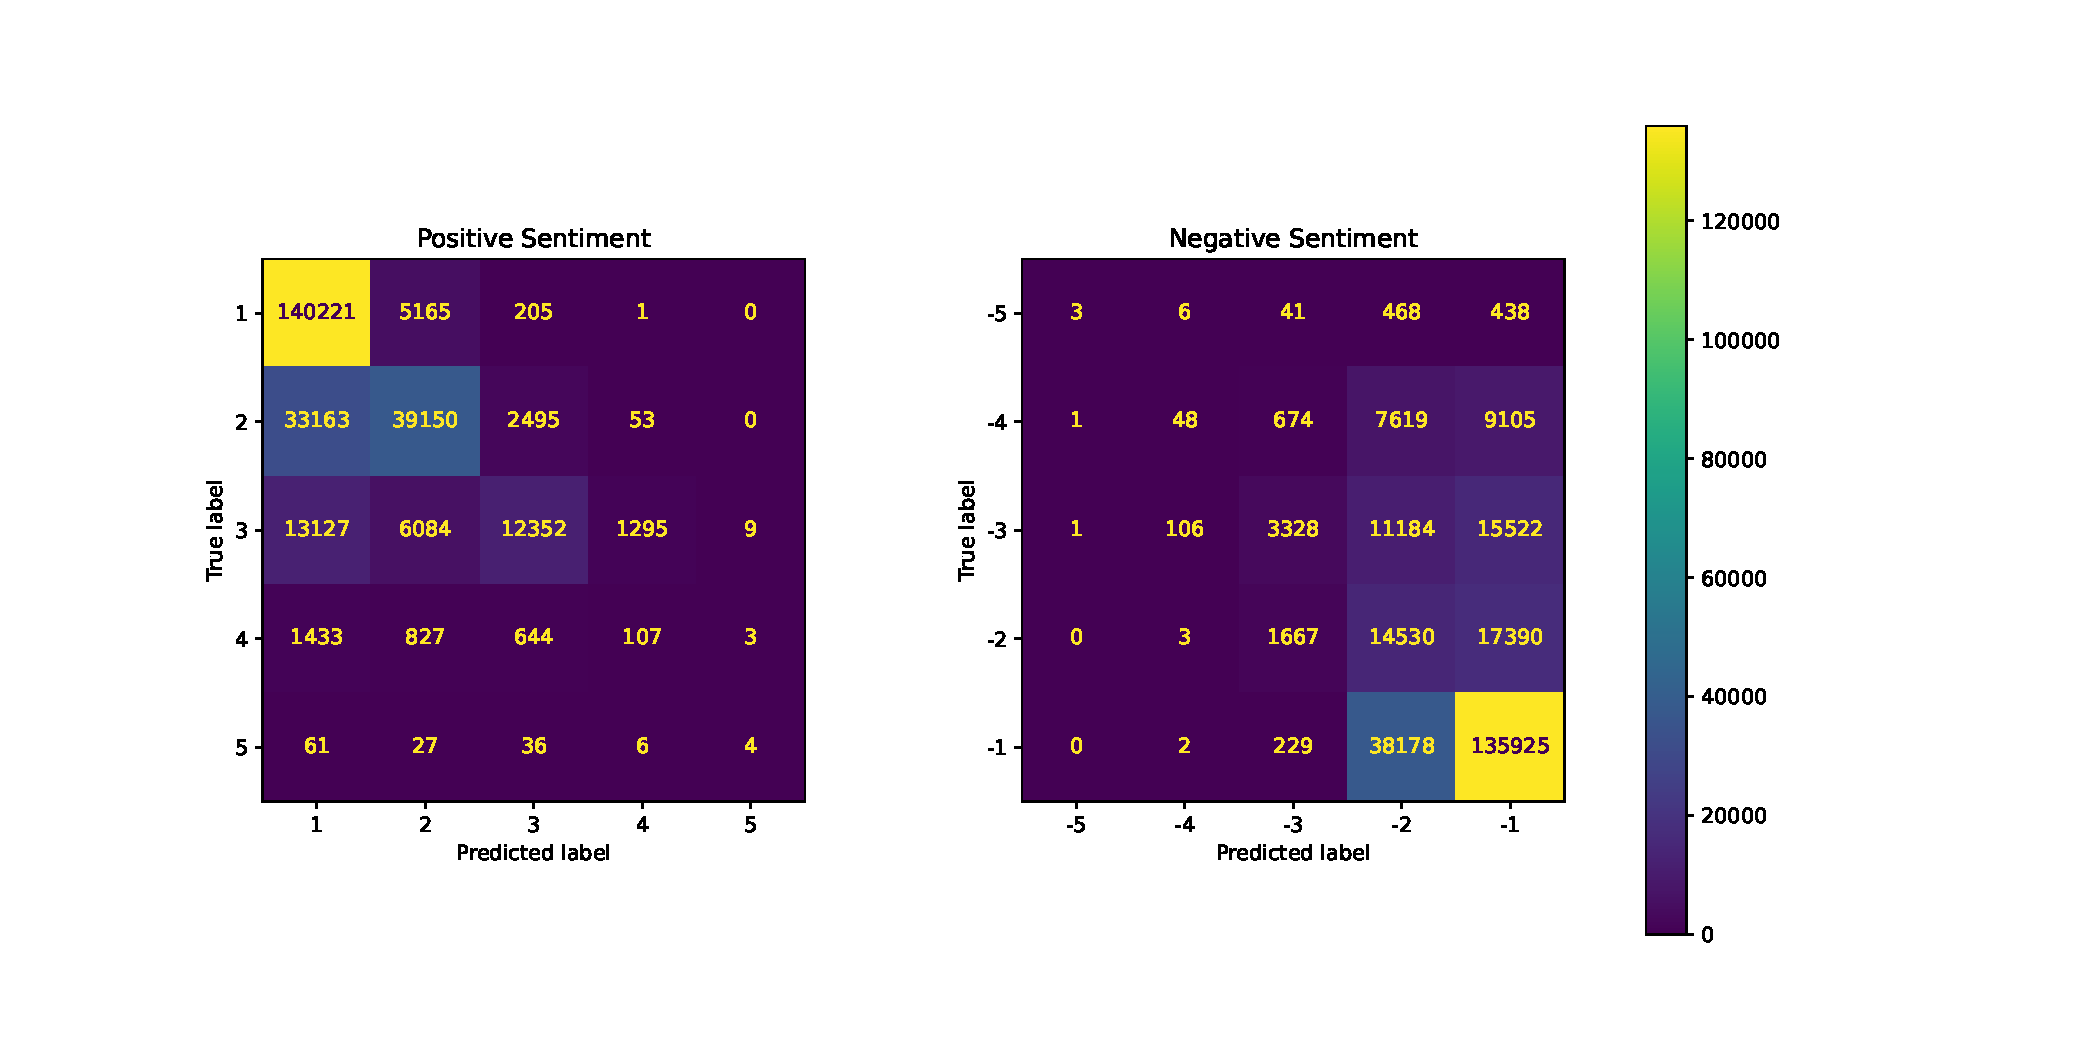
\includegraphics[width=\textwidth]{images/grad_boost_av_bow.pdf}
        \caption{Confusion matrix for the Gradient Boosting 'classifier' trained on BoW-embeddings that were aggregated by averaging.}    
        \label{fig:grad_boost_av_bow}
    \end{subfigure}
    \hfill
    \begin{subfigure}[b]{0.475\textwidth}
        \centering
        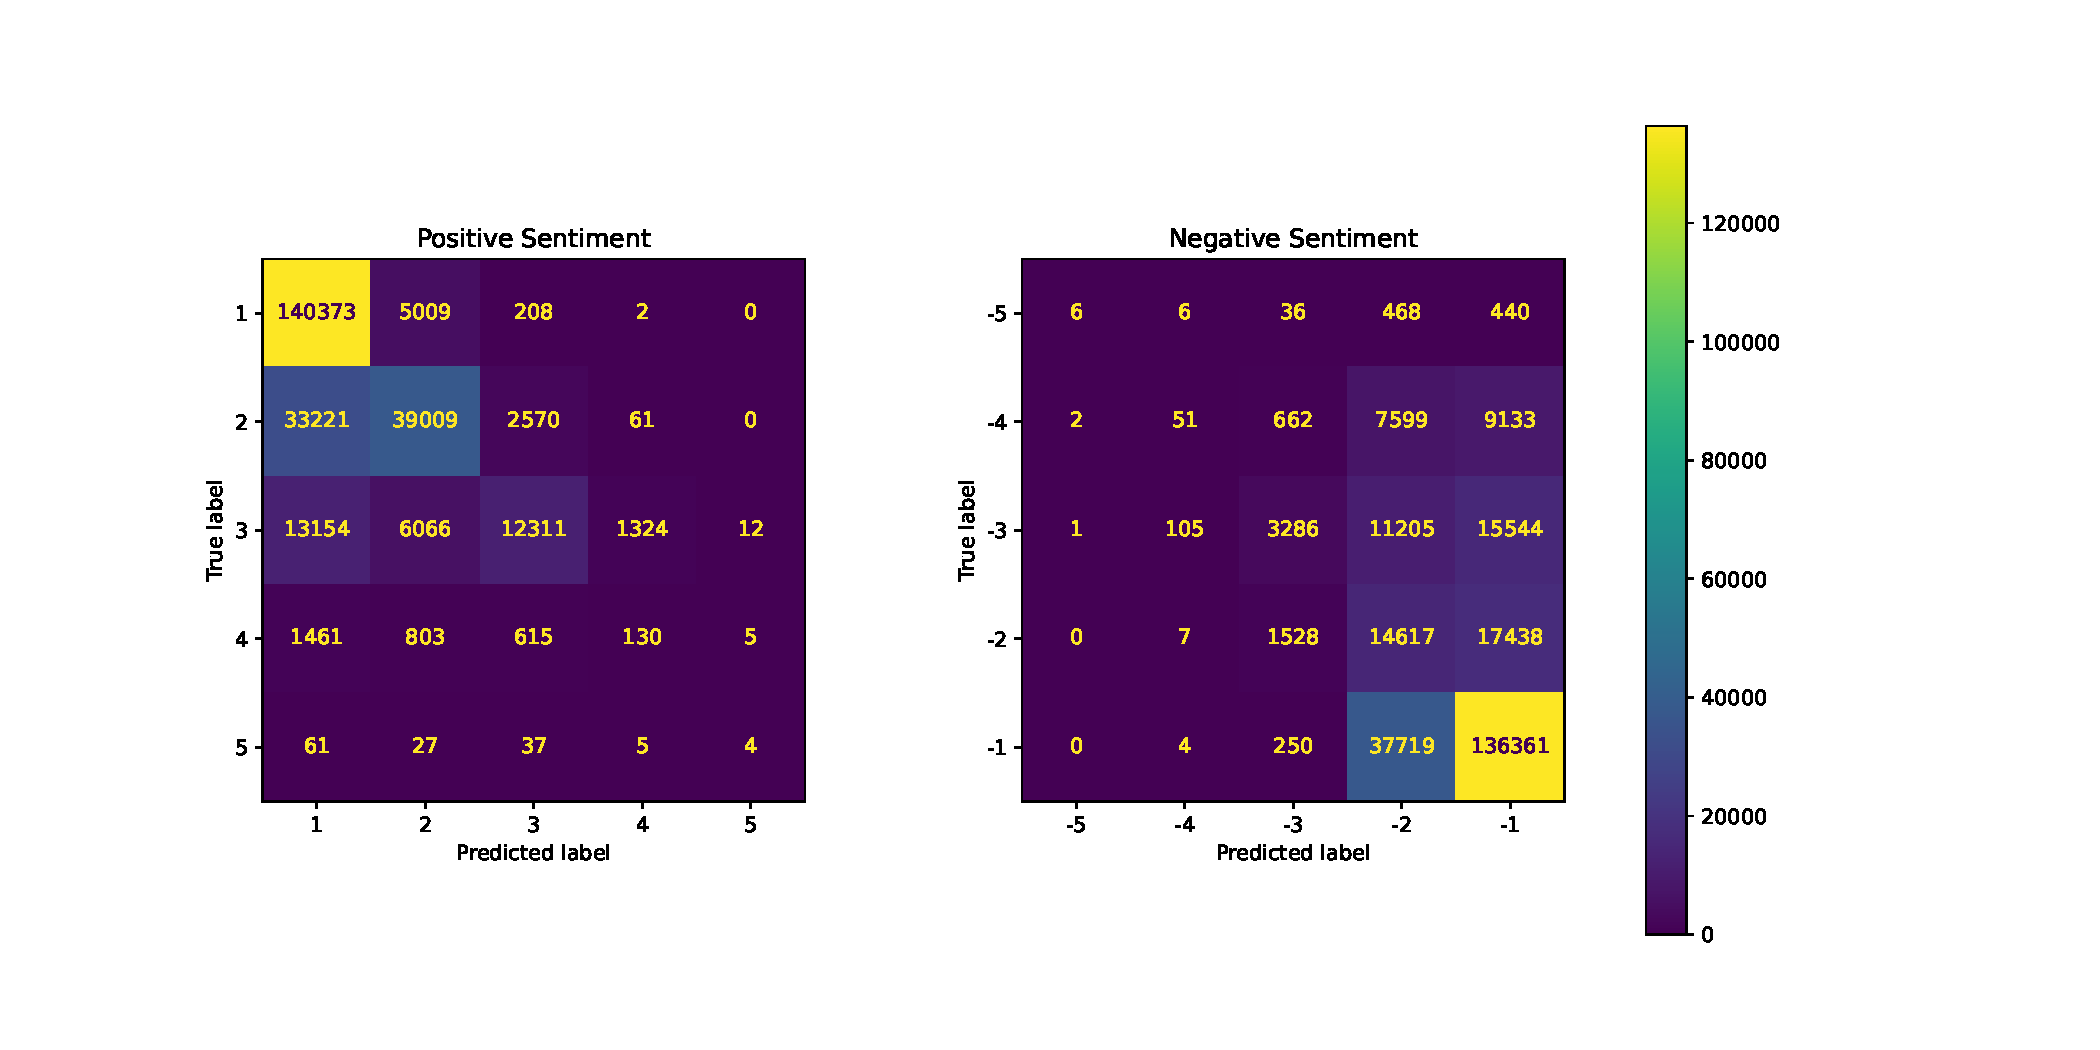
\includegraphics[width=\textwidth]{images/grad_boost_av_tfidf.pdf}
        \caption{Confusion matrix for the Gradient Boosting 'classifier' trained on TF-IDF-embeddings that were aggregated by averaging.}    
        \label{fig:grad_boost_av_tfidf}
    \end{subfigure}
    \vskip\baselineskip
    \begin{subfigure}[b]{0.475\textwidth}
        \centering
        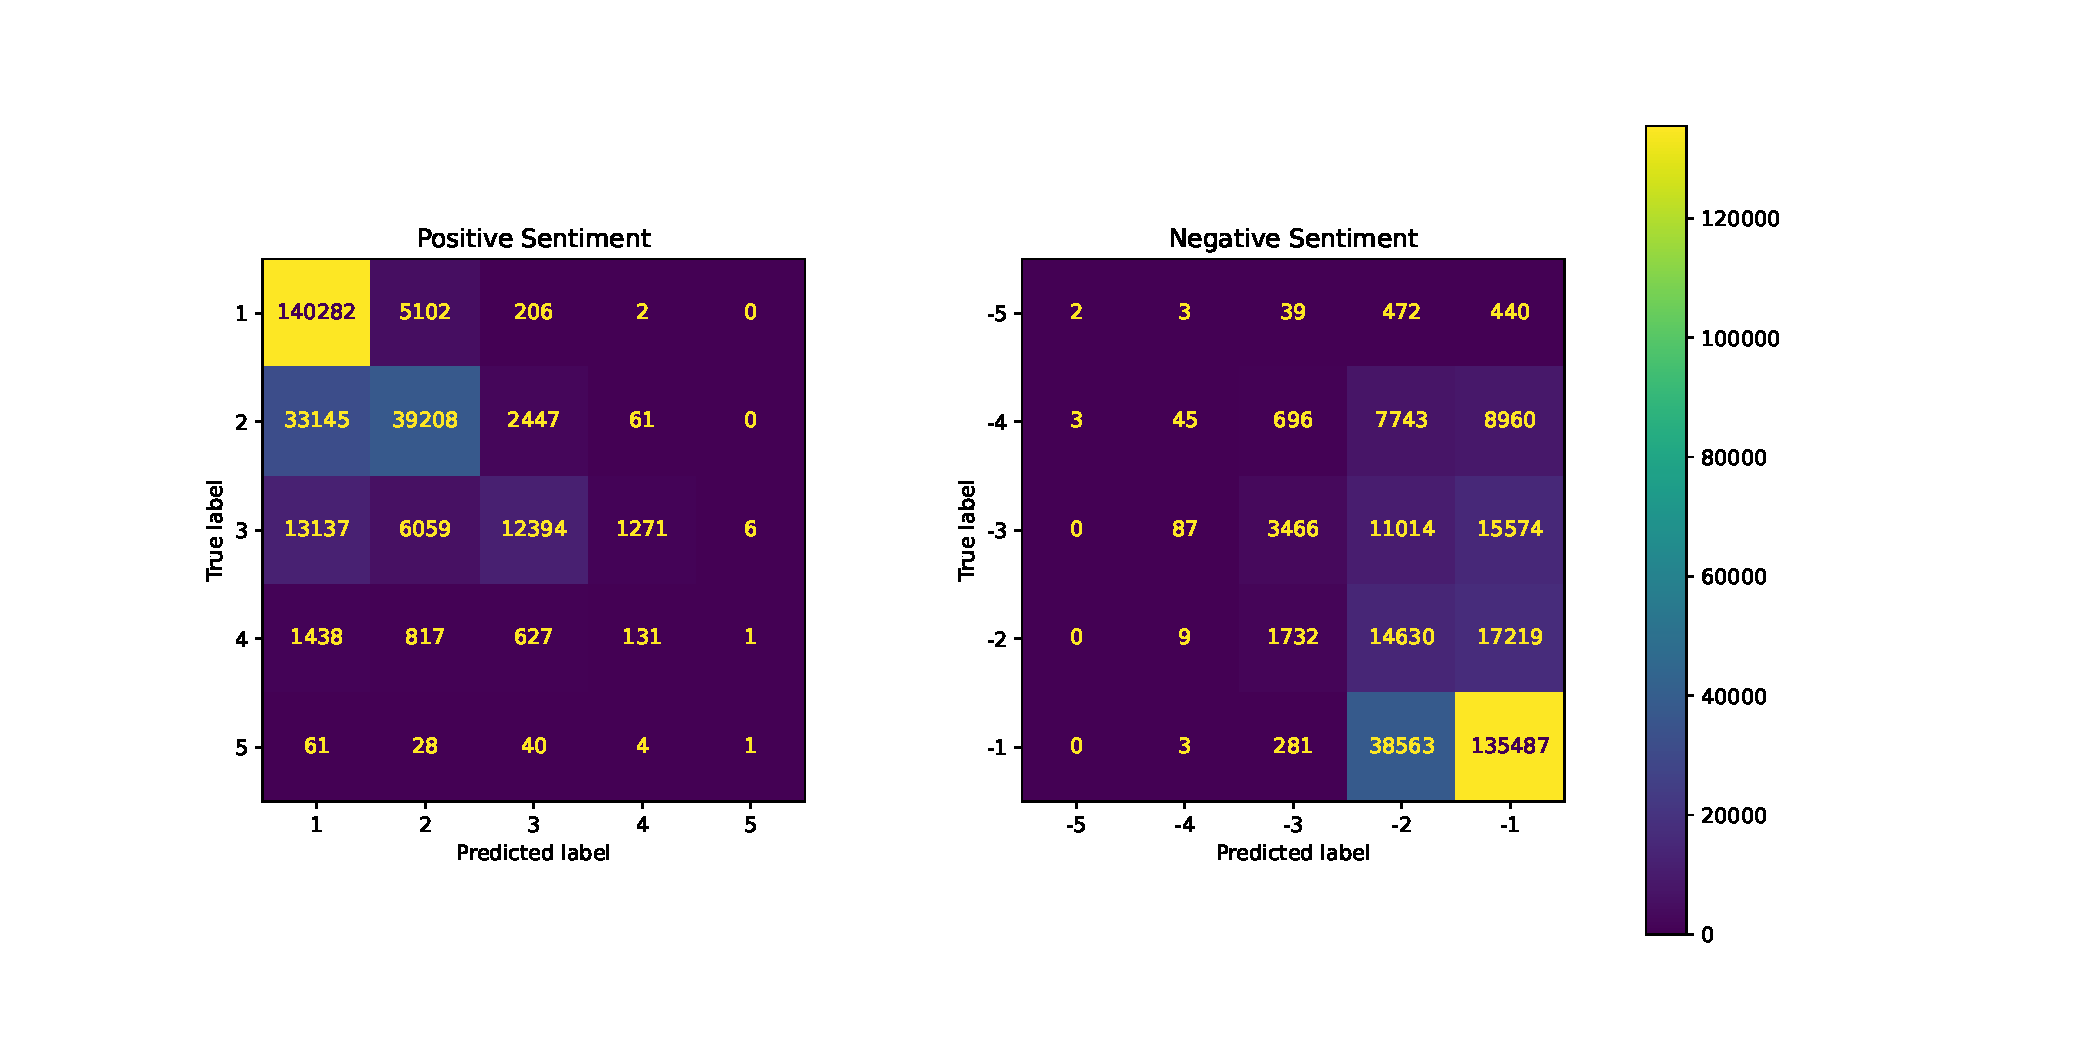
\includegraphics[width=\textwidth]{images/grad_boost_sum_bow.pdf}
        \caption{Confusion matrix for the Gradient Boosting 'classifier' trained on BoW-embeddings that were aggregated by summing.}    
        \label{fig:grad_boost_sum_bow}
    \end{subfigure}
    \hfill
    \begin{subfigure}[b]{0.475\textwidth}
        \centering
        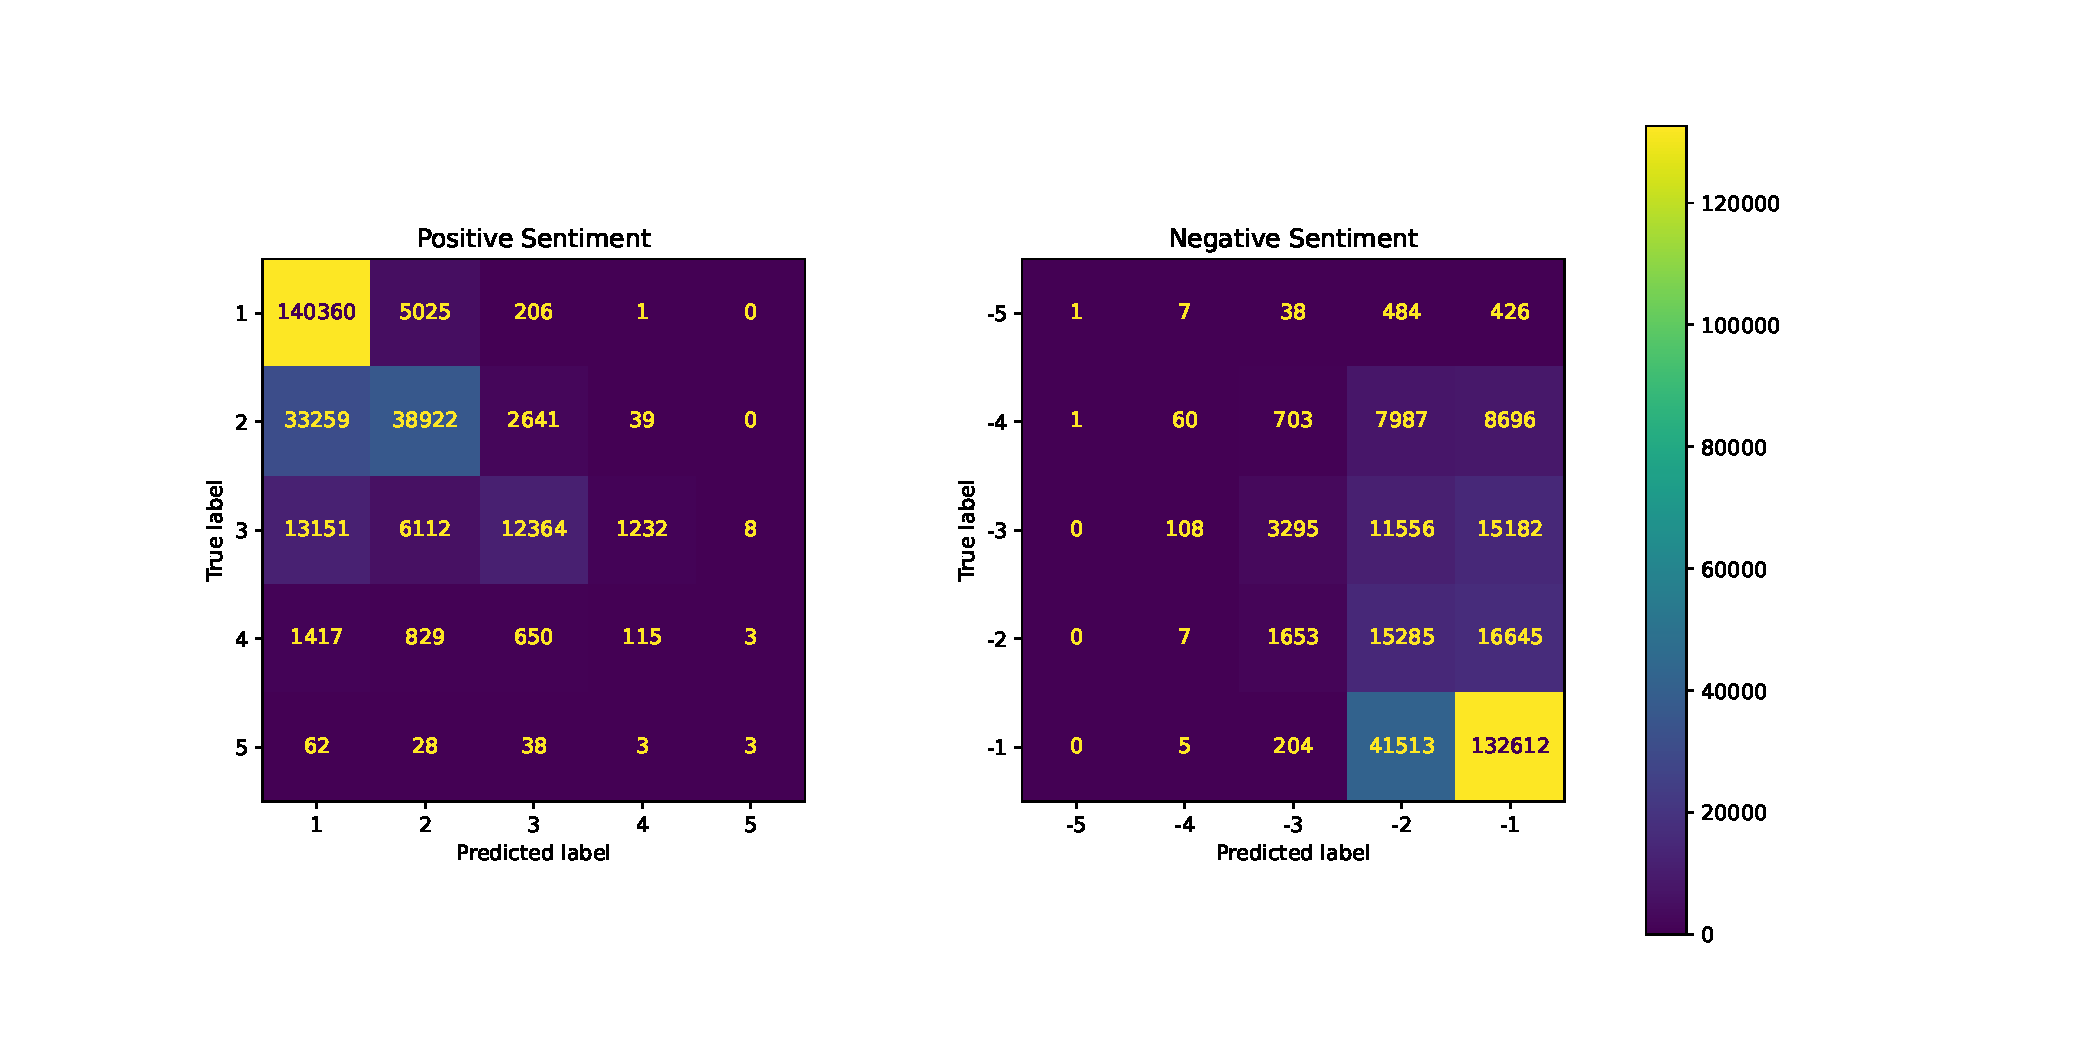
\includegraphics[width=\textwidth]{images/grad_boost_sum_tfidf.pdf}
        \caption{Confusion matrix for the Gradient Boosting 'classifier' trained on TF-IDF embeddings that were aggregated by summing.}    
        \label{fig:grad_boost_sum_tfidf}
    \end{subfigure}
   \vskip\baselineskip
    \begin{subfigure}[b]{0.475\textwidth}
        \centering
        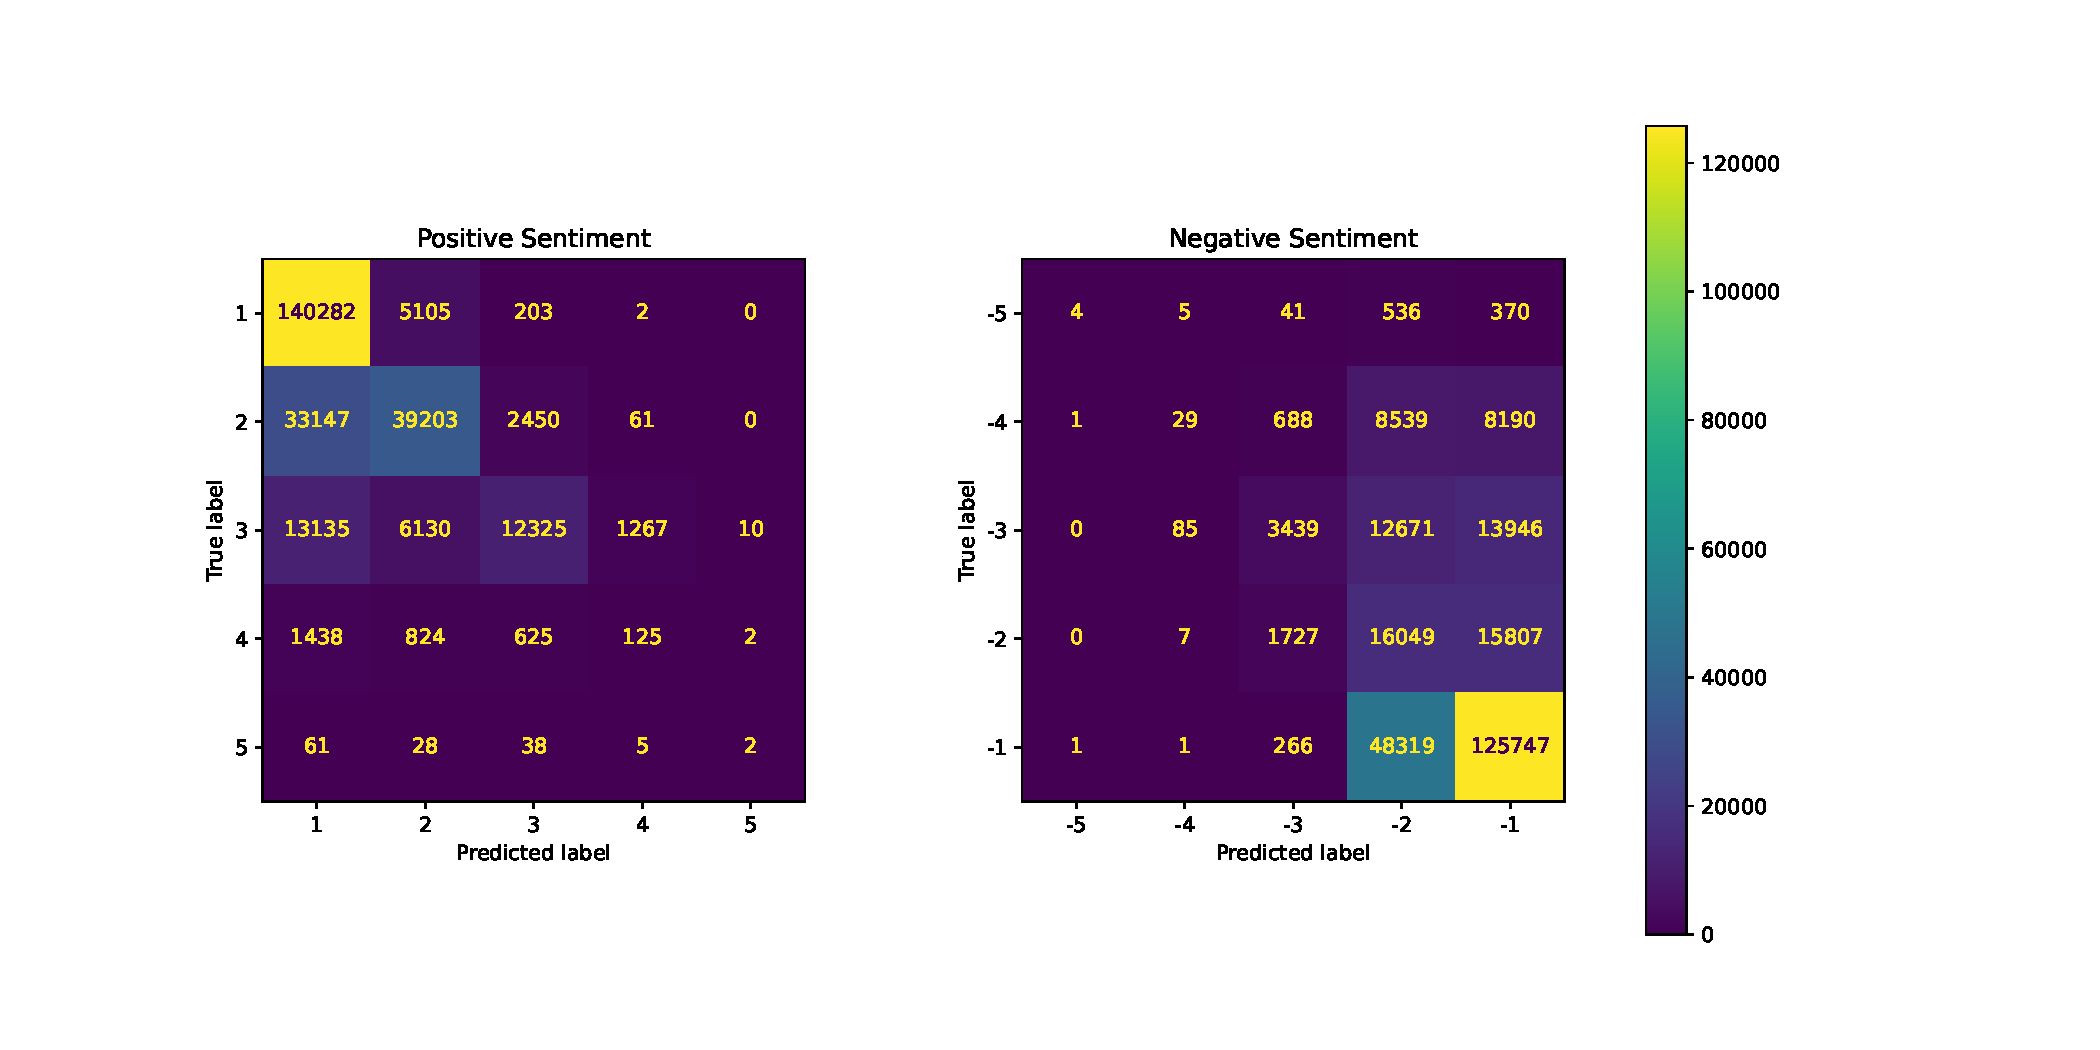
\includegraphics[width=\textwidth]{images/grad_boost_mm_bow.pdf}
        \caption{Confusion matrix for the Gradient Boosting 'classifier' trained on BoW-embeddings that were aggregated by concatenating the minimum and maximum over all word embeddings.}    
        \label{fig:grad_boost_mm_bow}
    \end{subfigure}
    \hfill
    \begin{subfigure}[b]{0.475\textwidth}
        \centering
        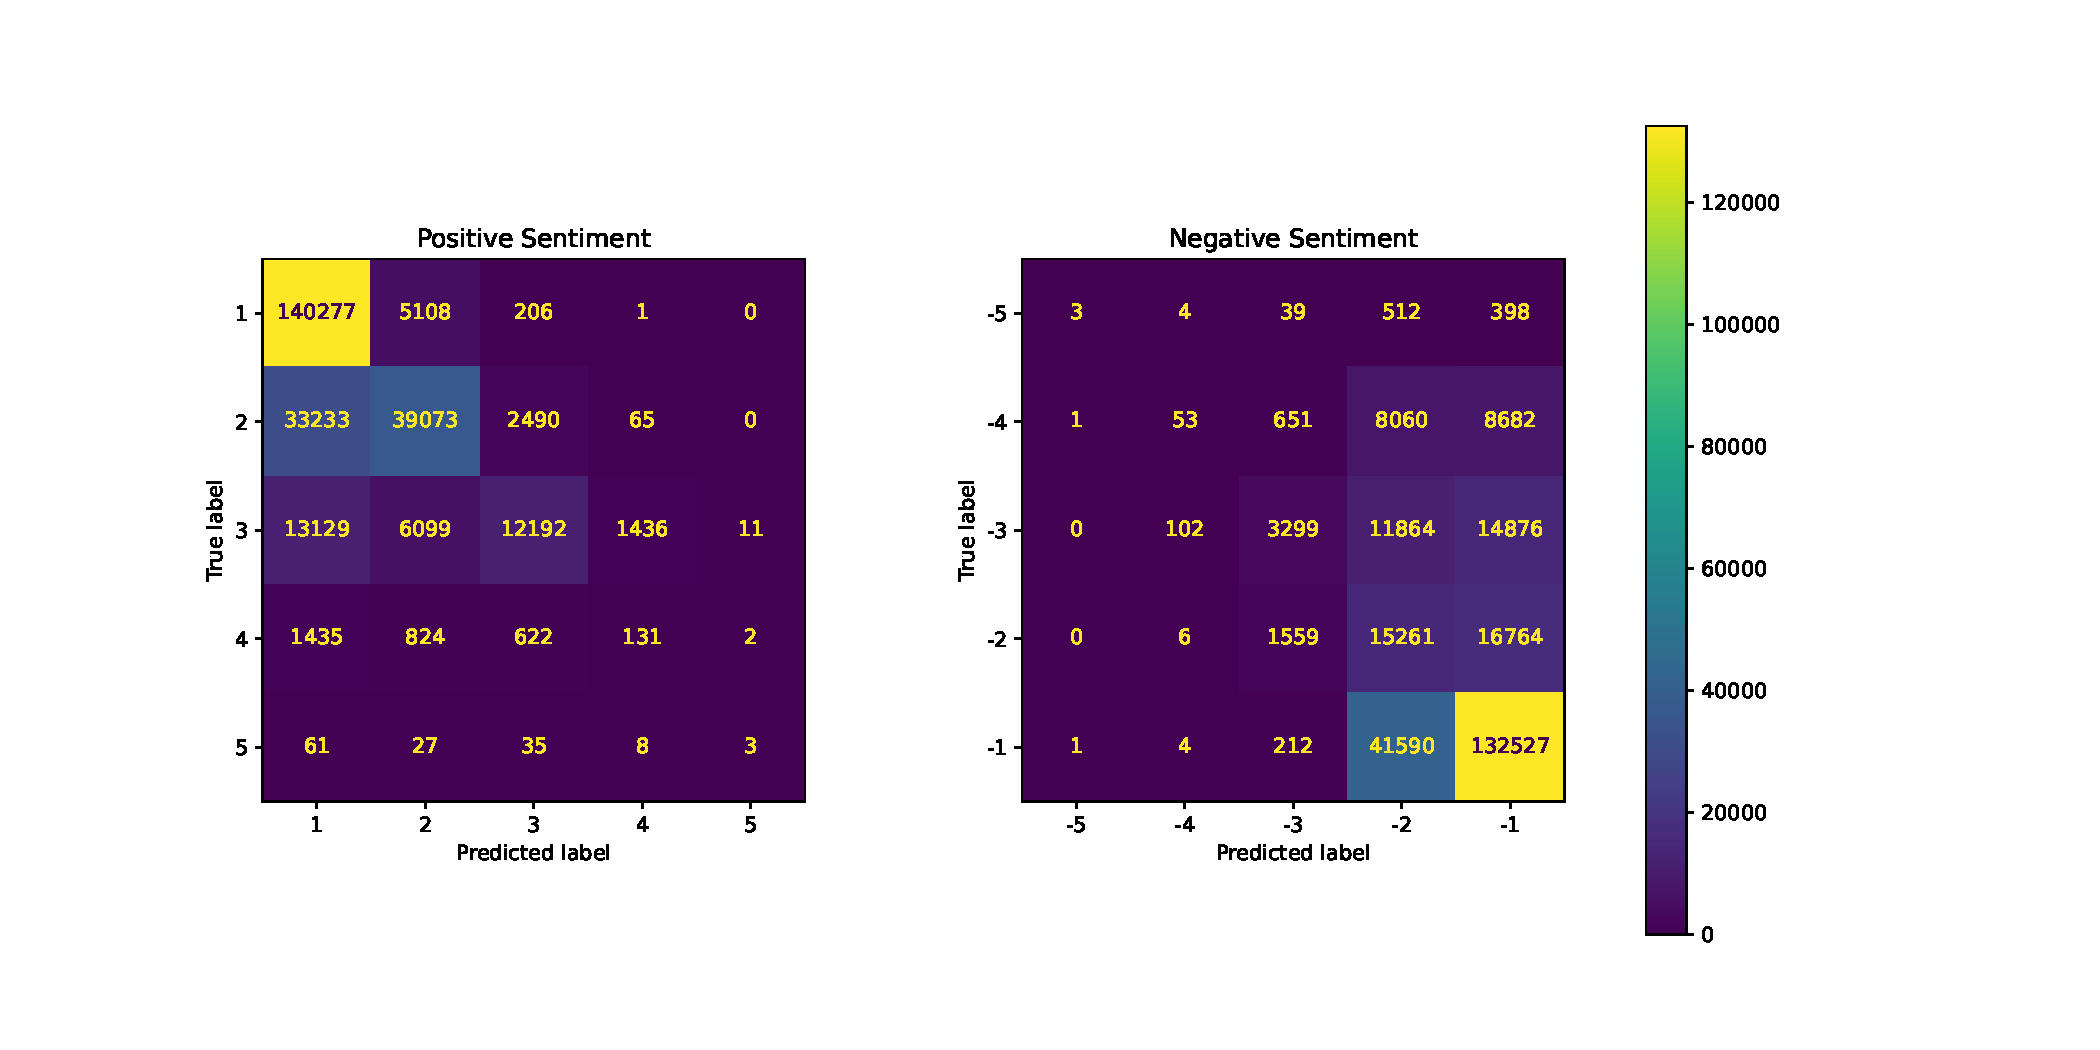
\includegraphics[width=\textwidth]{images/grad_boost_mm_tfidf.pdf}
        \caption{Confusion matrix for the Gradient Boosting 'classifier' trained on TF-IDF-embeddings that were aggregated by concatenating the minimum and maximum over all word embeddings.}
        \label{fig:grad_boost_mm_tfidf}
    \end{subfigure}
    \caption{Confusion matrices of six models trained with the Gradient Boosting algorithm. The models were selected based on a cutoff of $\ge 0.54$ for the training score (weighted harmonic F1 score).} 
    \label{fig:confusion_sklearn}
\end{figure*}

If we look at the confusion matrices of the models that have a final training score of $\ge 0.54$ (Figures \ref{fig:confusion_gensim} and \ref{fig:confusion_sklearn}), we see that (likely due to class imbalance), very positive and very negative tweets get misclassified most often. Therefore, we would like a model that prevents this somewhat.
Our final choice, taking our computational restrictions into account, is therefore to use TF-IDF for word embedding, averaging or summing as aggregation method, and Gradient Boosting as the training method. Although not the fastest, both these options strongly outperform most of the other models, even though the vocabulary size is limited.
Since OOV words cannot be accounted for with TF-IDF, a Gradient Boosting model trained with FastText embeddings aggregated by summing might still perform reasonably, and is thus considered a strong runner up for our final choice, especially since the vector size was limited in the embedding model.

As mentioned in the previous paragraph, one major thing we limited, was the final vector size of our embedding models. This was done to facilitate training. Still, for the Gensim models, the vector size we chose (v=20) vastly differs from the ones mentioned in the original papers (v=300), so using a larger vector size can potentially improve our results. The same holds for vocabulary size in the TF-IDF and BoW models, which we set at v=250. We expect some classifier results to improve when using larger feature vectors as input for the classification model.

In addition, we could try to train our very own convolutional neural network (CNN) for sentiment classification, which gives us much more flexibility than the usage of predefined models from existing libraries like scikit-learn.

Finally, we could look into classification vs. regression more in depth, and compare how 'real' classifiers perform, which would be especially useful to correct for class imbalance.

\clearpage 
\section*{\large Transformers}

\section{Transformer-based language models}

Transformer-based models are characteristic for using self-attention, which solves several bottlenecks in other models processing longer sequences of words/tokens. Unlike pure recurrent neural networks without self-attention mechanisms, self-attention heads in transformers allow the inference of the representation of input sequence tokens to focus on various other tokens of the input sequence equally. Without attention, the information from neighbouring tokens would vanish more easily with increasing distance between the tokens. Overall, this allows the representation of each token to be highly contextualised in the token sequence (such as a sentence), also if important relationships between input sequence tokens involve words that are far apart.

Some important architectural differences, which determine the number of parameters, are the following:
\begin{itemize}
    \item Training objectives. Language models differ in their objective functions, which determine the kind of tasks they would perform well.
    \item Building blocks in the model's architecture, such as self-attention heads, uni- or bi-directional long short-term memory units, gated recurrent units, etc.
    \item Size of the model, including number of hidden layers, number of connections between layers, sizes of embedding, sizes of hidden states of recurrent units, and the like.
    \item Training data and where they come from.
\end{itemize}
Below, we briefly compare the three models BERT, RoBERTa and GPT.

BERT and RoBERTa are similar models in that both are usually used in downstream tasks such as classification, language inference, question answering, and similar, with RoBERTa being a refined BERT model trained on a larger corpus. On the other hand, GPT is a generative model with the purpose of generating larger amounts of text.

BERT-based models are usually trained with masked language modelling and next-sentence prediction.
\begin{itemize}
    \item Masked language modelling means that the model is trained to correctly guess masked words from their context in both directions. Using a bidirectional transformer, the model can base the prediction of a masked token also on future tokens in the sequence.
    \item Next sequence prediction -- for a pair of sentences, the model learns to predict whether the sentences are consecutive.
\end{itemize}
In contrast to this, GPT models are trained to predict the next word in a sequence. Given a large corpus of human-generated text, training objectives are generated such that the model is given some prefix of a token sequence and trained to predict the next word of the sentence. The model uses a unidirectional transformer and so cannot make use of future tokens in the sentence for the prediction of the target token.

\section{Scalability}

Embedding-based models usually work on the word level and have a fixed embedding vector for each word. The embedding vectors are calculated during a much simpler training procedure, have a smaller number of parameters, and require smaller corpora.
As opposed to word embedding methods, transformer-based language models can produce contextualised embedding vectors for each input token which may lead to higher performance for a given task, but that entails much larger model sizes. Due to increased model complexity, transformer-based models require more computation resources and larger training datasets.

As for the trade-offs, embedding-based models can be more suitable for applications that require faster prediction, smaller memory usage, or lower computation resources. However, transformer-based models, if they can be afforded in terms of computation resources and available corpora, usually perform better.

\section{Code}

We chose to use the \texttt{distilbert-base-uncased-finetuned-sst-2-english} model which is a lightweight version of the BERT model with fewer parameters (only 6 hidden layers). Further, the model is fine-tuned for sentiment classification, so it should perform well even without much training.

However, our task is different from the usual sentiment analysis: we need two outputs, one for positive and one for negative sentiment variable. This will require at least some training, since we are constructing new layers with a different number of parameters than the standard model.

Further, we chose to model this as a regression problem, even though the reported metric will be the classification metric \textit{Weighted-F1 HM}. Therefore we use the \textit{MSE} loss for both sentiment variables, adding the loss values together, to optimise the regression.

First, as shown in \cref{listing:p2t-regression-model}, we create a new class \texttt{TFDistilBertForSentiStrengthRegression}, subclassing from \texttt{TFDistilBertForSequenceClassification}. Our code, as opposed to its super class, modifies the last two layers. We use the following last layers:
\begin{itemize}
    \item A hidden layer with the size of 768 (the default hidden state size for distilbert) with the ReLU activation function, similar to previous hidden layers of the model. This layer takes as input the embedding corresponding to the \texttt{[CLS]} token, i.e. the embedding that is trained to capture the sentiment of the whole sentence. This is done in the same way as the \texttt{TFDistilBertForSequenceClassification} model.
    \item An output layer with two outputs, one for each sentiment variable. Since we are modelling the problem as regression directly of the given values, we apply no activation function on the two output neurons (i.e. \textit{linear}).
\end{itemize}

Further, in \cref{listing:p2t-build-model} we demonstrate how to build the model, with a custom number of layers that are set as trainable. The included \texttt{build\_model} function does the following:
\begin{itemize}
    \item Initialize the \texttt{TFDistilBertForSentiStrengthRegression}
    \item Based on the provided argument, the function iterates through the layers of the pre-trained model and sets them as trainable respectively. By default, none of the pre-trained layers will be set as trainable.
    \item Compiles the model with the Adam optimizer, using the \texttt{mse\_sum} loss function that adds the MSE loss value of the two sentiment variables.
\end{itemize}
In \cref{listing:p2t-build-model-call} we show how to call the \texttt{build\_model} function to construct the model once with fixed pre-trained layers, and once with the last pre-trained layer to be fine-tuned, too.

Finally, in \cref{listing:p2t-model-train} we show how to train the model.

\begin{listing*}
\caption{A code snipped showing our implementation of \texttt{TFDistilBertForSentiStrengthRegression}.}
\begin{minted}{python}
from transformers import TFDistilBertMainLayer
from transformers.modeling_tf_utils import get_initializer, unpack_inputs, TFModelInputType
from transformers.utils.generic import ModelOutput
from typing import Optional, Union, Tuple
from dataclasses import dataclass

@dataclass
class TFSentiStrengthRegressionOutput(ModelOutput):
    loss: Optional[tf.Tensor] = None
    values: Optional[tf.Tensor] = None
    hidden_states: Optional[Tuple[tf.Tensor]] = None
    attentions: Optional[Tuple[tf.Tensor]] = None

class TFDistilBertForSentiStrengthRegression(TFDistilBertForSequenceClassification):
    def __init__(self, config, *inputs, **kwargs):
        super(TFDistilBertForSequenceClassification, self).__init__(config, *inputs, **kwargs)

        self.distilbert = TFDistilBertMainLayer(config, name="distilbert")
        self.pre_regression = tf.keras.layers.Dense(
            config.dim,
            kernel_initializer=get_initializer(config.initializer_range),
            activation="relu",
            name="pre_regression",
        )
        self.regression = tf.keras.layers.Dense(
            units=2, kernel_initializer=get_initializer(config.initializer_range), name="regression",
            activation='linear'
        )
        self.dropout = tf.keras.layers.Dropout(config.seq_classif_dropout)

    @unpack_inputs
    def call(
            self,
            input_ids: Optional[TFModelInputType] = None,
            attention_mask: Optional[Union[np.ndarray, tf.Tensor]] = None,
            head_mask: Optional[Union[np.ndarray, tf.Tensor]] = None,
            inputs_embeds: Optional[Union[np.ndarray, tf.Tensor]] = None,
            output_attentions: Optional[bool] = None,
            output_hidden_states: Optional[bool] = None,
            return_dict: Optional[bool] = None,
            labels: Optional[Union[np.ndarray, tf.Tensor]] = None,
            training: Optional[bool] = False,
    ) -> Union[TFSentiStrengthRegressionOutput, Tuple[tf.Tensor]]:
        distilbert_output = self.distilbert(
            input_ids=input_ids,
            attention_mask=attention_mask,
            head_mask=head_mask,
            inputs_embeds=inputs_embeds,
            output_attentions=output_attentions,
            output_hidden_states=output_hidden_states,
            return_dict=return_dict,
            training=training,
        )
        hidden_state = distilbert_output[0]  # (bs, seq_len, dim)
        pooled_output = hidden_state[:, 0]  # (bs, dim)
        pooled_output = self.pre_regression(pooled_output)  # (bs, dim)
        pooled_output = self.dropout(pooled_output, training=training)  # (bs, dim)
        values = self.regression(pooled_output)  # (bs, dim)

        loss_fn = tf.keras.losses.MeanSquaredError(reduction=tf.keras.losses.Reduction.NONE)
        loss = None if labels is None else loss_fn(labels, values)

        if not return_dict:
            output = (values,) + distilbert_output[1:]
            return ((loss,) + output) if loss is not None else output

        return TFSentiStrengthRegressionOutput(
            loss=loss,
            values=values,
            hidden_states=distilbert_output.hidden_states,
            attentions=distilbert_output.attentions,
        )
\end{minted}
\label{listing:p2t-regression-model}
\end{listing*}

\begin{listing*}
\caption{A code snipped showing how to build and compile the tensorflow model.}
\begin{minted}{python}
def build_model(trainable_last_layers=0):
    custom_bert = TFDistilBertForSentiStrengthRegression.from_pretrained(MODEL_NAME)
    if trainable_last_layers > 0:
        custom_bert.distilbert.trainable = True
        custom_bert.distilbert.embeddings.trainable = False
        for layer in custom_bert.distilbert.transformer.layer[0:-trainable_last_layers]:
            layer.trainable = False
    else:
        custom_bert.distilbert.trainable = False

    input_ids = tf.keras.layers.Input(shape=(None,), dtype=tf.int32, name="input_ids")
    outputs = custom_bert(input_ids).values

    model = tf.keras.models.Model(
        inputs=[input_ids],
        outputs=[outputs],
        name=MODEL_NAME_SHORT,)

    def mse_sum(y_true, y_pred):
        return tf.keras.metrics.mean_squared_error(y_true[0], y_pred[0]) + tf.keras.metrics.mean_squared_error(y_true[1], y_pred[1])
    def mae_sum(y_true, y_pred):
        return tf.keras.metrics.mean_absolute_error(y_true[0], y_pred[0]) + tf.keras.metrics.mean_absolute_error(y_true[1], y_pred[1])
    def mae_pos(y_true, y_pred):
        return tf.keras.metrics.mean_absolute_error(y_true[0], y_pred[0])
    def mae_neg(y_true, y_pred):
        return tf.keras.metrics.mean_absolute_error(y_true[1], y_pred[1])

    model.compile(
        optimizer=tf.keras.optimizers.Adam(learning_rate=1e-3),
        loss=mse_sum,
        metrics=[mae_sum, mae_pos, mae_neg],)
    return model
\end{minted}
\label{listing:p2t-build-model}
\end{listing*}

\begin{listing*}
\caption{A code snipped showing how to call the \texttt{build\_model} function.}
\begin{minted}{python}
# DistilBERT with fixed pre-trained layers, only set to train the added regression layers
model_fixed = build_model(trainable_last_layers=0)
# DistilBERT also allowing the last pre-trained layer to be fine-tuned
model_refined1 = build_model(trainable_last_layers=1)
\end{minted}
\label{listing:p2t-build-model-call}
\end{listing*}

\begin{listing*}
\caption{A code snipped showing how to train the model.}
\begin{minted}{python}
def train_model(name, model, epochs=10, train_data=train_data, val_data=val_data):
    # Create callbacks
    metrics = ... # A callback that calculates our metrics (including val_f1w_hm) on the validation dataset
    model_checkpoint_callback = ... # Save the model after every epoch
    tensorboard_callback = ...

    history = model.fit(
        x=train_data,
        validation_data=val_data,
        epochs=epochs,
        callbacks=[
            ...
        ],
    )
    return history

history_fixed = train_model('fixed', model_fixed, epochs=8)
\end{minted}
\label{listing:p2t-model-train}
\end{listing*}


\section{Performance analysis}

As per \cref{listing:p2t-model-train}, we trained the two models (fixed, and with last 

\clearpage 
\section*{\large Part 3: Downstream Global Health Analysis}
\section{Downstream Global Health Analysis}

\subsection*{Q1: Research question (2 pts)}
\textit{Among the papers in the project instructions, identify a research question they address that you could explore using the TweetsCOV19 dataset. For example, set out to analyze sentiments towards Covid-19 as a function of time or geographical location, or of any sub-topic related to the pandemic. Motivate the relevance of your question in the context of the pandemic. Feel free to use another peer-reviewed paper analyzing COVID tweets for public health insights for inspiration. Ensure to provide a correct citation.}

We have chosen to look at the paper “How epidemic psychology works on Twitter: evolution of responses to the COVID-19 pandemic in the U.S.“ by Aiello, L.M., Quercia, D., Zhou, K. et al. \cite{aiello2021epidemic}. We choose to look at the evolution in time of sentiment and emotion with regards to COVID-19, in the United States. 

The paper focuses on a theory called “Epidemic Psychology” by Philip Strong \cite{strong1990epidemic}, which is a sociological study of psycho-social ‘epidemics’ of fear, moralization and action that occur during major health epidemics. The authors wish to observe whether they can empirically observe these phases of emotion spreading as an epidemic through language, through the analysis of tweets, during the COVID-19 pandemic. 

Analyzing the evolution of emotion and sentiment throughout the COVID-19 pandemic through the use of tweets is a very important undertaking, as it helps inform future public health policies. Indeed, as information dissemination is extremely rapid nowadays, the spreading of fear, panic, and the amplifying misinformation, is a grave danger to public health messaging. Understanding past trends can help prevent these feelings that ultimately have a big impact on policy. Finally, we also choose to focus on the US as per the paper, as the US has the highest proportion of Twitter users, and because it is easier to relate evolution of emotions in time to the events of a single country.


\subsection*{Q2: Method choice and design (5 pts).}
\textit{Among the methods you have explored in Part 2, select one approach to tackle this research question using the TweetsCOV19 dataset and motivate your choice. Detail any necessary modifications you implement to achieve this analysis and performance metrics to measure the success of your approach. Provide a code snippet used to perform this analysis.}
TODO @Juraj

\subsection*{Q3: Results \& Analysis (6 pts).}
\textit{ Analyze your results and provide numerical evaluation and visualizations showcasing your findings. (3 pts) Explain what conclusions can be drawn from these, as well as key takeaways which answer (or partially answer) your research question. (3 pts)}
TODO @Juraj


\subsection*{Q4: Comparison to literature (3 pts).}
\textit{ Discuss whether your results support or disagree with the paper you have chosen for inspiration. Provide plausible reasons for different findings or any performance discrepancies.}
TODO @Juraj


\subsection*{Q5: Discussion (3 pts).}
\textit{ Discuss the pros and cons of your approach compared to the one used in the paper.}
TODO @Juraj


\subsection*{Q6: Summary \& Conclusion (1 pt).}
\textit{ Provide a summary of your analysis and the insights it provides about your research question.}
TODO @Juraj

\clearpage 
\section*{\large Bonus: Topic \& Emotion Analysis}
\section*{Bonus: Topic \& Emotion Analysis (+5 pts)}

\subsection{Topic Modeling}
\textit{Perform a topic modeling using the Latent Dirichlet Allocation (LDA) approach. Explain the foundations of this approach and provide the code snippet used to apply this method. Finally provide a visualization of your results and detail the conclusions you can draw about the COVID-19 epidemics using topic modeling. Compare your results with the Nature article which performs a similar analysis. Hypothesize on why results might be different.}

Latent Dirichlet allocation (LDA) \cite{lda} is a method used to infer topics from text. These topics are not known in advance, and are supposed to be inferred from the words that are grouped under them after training of the model.

\begin{listing*}[t]
\begin{minted}{python}
! pip install pyLDAvis

from gensim.corpora.dictionary import Dictionary
from gensim.models import LdaModel,CoherenceModel
import pyLDAvis
import pyLDAvis.gensim

diction = Dictionary(df_tweets_preprocessed['unigram'])
corpus = [diction.doc2bow(i) for i in df_tweets_preprocessed['unigram']]
n_topics = 4
lda = LdaModel(corpus, id2word=diction, num_topics=n_topics, random_state=42, passes=2)

#inspired by https://www.machinelearningplus.com/nlp/topic-modeling-gensim-python/
# Compute Perplexity
print('\nPerplexity: ', lda.log_perplexity(corpus))  # a measure of how good the model is. lower the better.

# Compute Coherence Score
coherence_model_lda = CoherenceModel(model=lda, texts=df_tweets_preprocessed['unigram'], dictionary=diction, coherence='c_v')
coherence_lda = coherence_model_lda.get_coherence()
print('\nCoherence Score: ', coherence_lda)

pyLDAvis.enable_notebook()
vis = pyLDAvis.gensim.prepare(lda, corpus, diction,R=10)
vis

\end{minted}
\caption{}
\label{listing:pb-code1}
\end{listing*}


We inferred the following topics from LDA: covid safety rules (containing words such as: 'stay' and 'home', 'social' and 'distancing', 'mask'), government and politics (containing words like: 'Trump', 'lockdown', 'president', and 'pm' ), news reports (containing words like 'new' and 'cases', 'pandemic', 'death', 'China'), and a covid-related topic we could not find a common term for (containing words such as 'quarantine', 'know', 'like', 'thing', 'lockdown', 'day', and 'one'). The histogram of the topic frequencies can be found in Figure \ref{fig:lda_histo}, and the words related to each topic can be found in Figure \ref{fig:lda_viz}

\begin{figure}
 \centering
 \begin{subfigure}{0.5\columnwidth}
 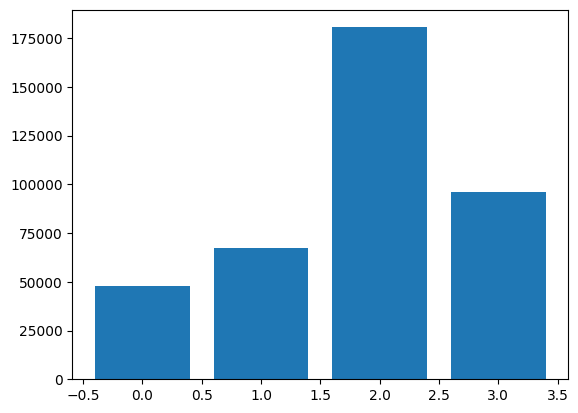
\includegraphics[width=1\textwidth]{images/LDA_topics.png}
 \end{subfigure}
 \caption{Most common topics in the TweetsCov19 dataset. Topic 1 corresponds to the unknown topic, topic 2 to 'news reports', topic 3 to 'covid safety rules', and topic 4 to 'government and politics'.}
 \label{fig:lda_histo}
\end{figure}


Different from the Nature article \cite{ldaUK}, we were unable to find more than 4 sensible topics, with topics beyond 3 often strongly overlapping with one another. This is likely due to the fact that we are using a different dataset and different preprocessing methods. Their dataset is almost double the size (800 000 tweets), and contains tweets from the UK only, while ours contains tweets from across the world (the majority from the US, which is probably a big reason why Trump is so prominent in one of the topics)


\begin{figure}
 \centering
 \begin{subfigure}{0.75\columnwidth}
 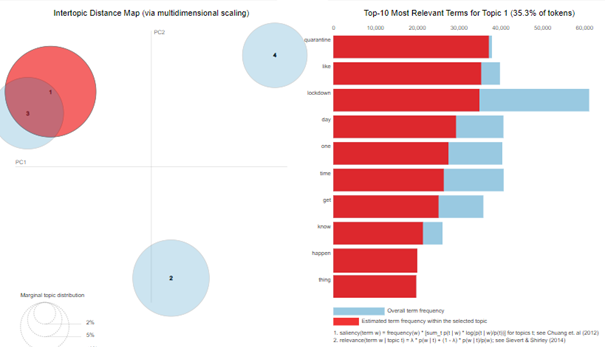
\includegraphics[width=1\textwidth]{images/lda1.png}
 \end{subfigure}
 \centering
 \begin{subfigure}{0.75\columnwidth}
 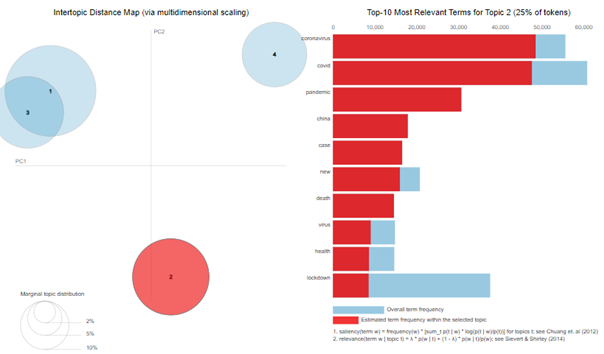
\includegraphics[width=1\textwidth]{images/lda2.png}
 \end{subfigure}
 \caption{Visualization of the topics inferred from LDA. Topic 1 corresponds to the unknown topic and topic 2 to 'news reports'.}
 \label{fig:lda_viz}
\end{figure}



\begin{figure}
 \ContinuedFloat
 \centering
 \begin{subfigure}{0.75\columnwidth}
 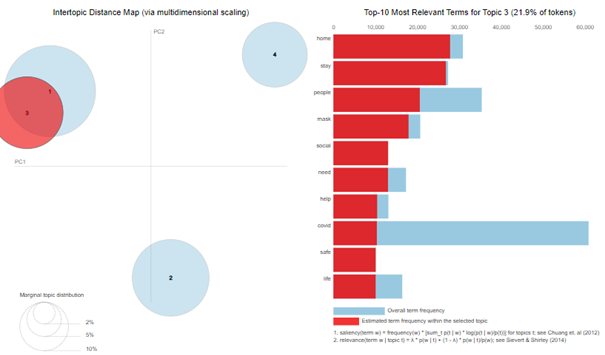
\includegraphics[width=1\textwidth]{images/lda3.png}
 \end{subfigure}
 \centering
 \begin{subfigure}{0.75\columnwidth}
 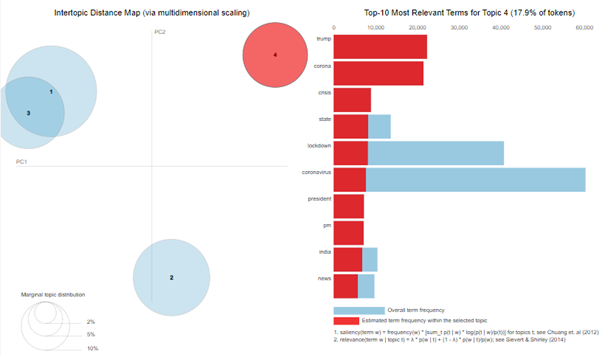
\includegraphics[width=1\textwidth]{images/lda4.png}
 \end{subfigure}
 \caption{(continued) Visualization of the topics inferred from LDA. Topic 3 corresponds to 'covid safety rules', and topic 4 to 'government and politics'.}
 \label{fig:lda_viz}
\end{figure}




\clearpage

%\printbibliography
\printbibliography[heading=references]

\end{document}
